\documentclass[10pt,a4paper,openright]{book}

%% Formateo del título del documento
\title{\Huge CÁLCULO DIFERENCIAL}
\author{Juan Diego Barrado Daganzo e Iker Muñoz Martínez\\2º de Carrera} %\\ es salto de linea
\date{\today\footnote{Este documento se actualiza, para consultar las últimas versiones entrar en el enlace \url{https://github.com/JuanDiegoBarrado/CalculoDiferencial}}}

%% Formateo del estilo de escritura y de la pagina
\pagestyle{plain}
\setlength{\parskip}{0.35cm} %edicion de espaciado
\setlength{\parindent}{0cm} %edicion de sangría
\clubpenalty=10000 %líneas viudas NO
\widowpenalty=10000 %líneas viudas NO
\usepackage[top=2.5cm, bottom=2.5cm, left=3cm, right=3cm]{geometry} % para establecer las medidas de los margenes
\usepackage[spanish]{babel} %Para que el idioma por defecto sea español
\usepackage{ulem} % para poder subrayar entornos especiales como las secciones

%% Texto matematico y simbolos especiales
\usepackage{amsmath} %Paquetes para mates
\usepackage{amsfonts} %Paquetes para mates
\usepackage{amssymb} %Paquetes para mates
\usepackage{stmaryrd} % paquete para mates
\usepackage{latexsym} %Paquetes para mates
\usepackage{cancel} %Paquete tachar cosas

%% Ruta de las fotos e inclusion de las mismas
\usepackage{graphicx}
\graphicspath{{./fotos/}}

%% Paquete para subfigures dentro del entorno figure
\usepackage{subcaption}

%% Inclusion de referencias cruzadas por defecto y específicas
\usepackage{hyperref}

%% Paquete para definir y utilizar colores por el documento
\usepackage[dvipsnames,usenames]{xcolor} %activar e incluir colores
	%% definicion de los colores que se van a utilizar en cada cabecera
    \definecolor{capitulos}{RGB}{60,0,0}% gama de colores de los capitulos
    \definecolor{secciones}{RGB}{95,8,5}% gama de colores de las secciones
    \definecolor{subsecciones}{RGB}{140,36,31}% gama de colores de las subsections
    \definecolor{subsubsecciones}{RGB}{188,109,79}% gama de colores de las subsubsections
    \definecolor{teoremas}{RGB}{164,56,32}% gama de colores para los teoremas
    \definecolor{demos}{RGB}{105,105,105} % gama de colores para el cuerpo de las demostraciones
    
%% Paquete para la edición y el formateo de capítulos, secciones...
\usepackage[explicit]{titlesec}
	%% Definición del estilo de los capítulos, secciones, etc...
    \titleformat{\chapter}[display]{\normalfont\huge\bfseries\color{capitulos}}{}{0pt}{\Huge #1}[\titlerule]
    \titleformat{\section}{\normalfont\Large\bfseries\color{secciones}}{}{0pt}{#1}
    \titleformat{\subsection}{\normalfont\large\bfseries\color{subsecciones}}{}{0pt}{\uline{#1}}
    \titleformat{\subsubsection}{\normalfont\normalsize\bfseries\color{subsubsecciones}}{}{0pt}{#1}
    
%% Paquete para el formateo de entornos del proyecto
\usepackage{ntheorem}[thmmarks]
	%% Definicion del aspecto de los entornos matematicos del proyecto
	\theoremstyle{break}
	\theoremheaderfont{\normalfont\bfseries\color{teoremas}}
	\theorembodyfont{\itshape}
	\theoremseparator{\vspace{0.2cm}}
	\theorempreskip{\topsep}
	\theorempostskip{\topsep}
	\theoremindent0cm
	\theoremnumbering{arabic}
	\theoremsymbol{}
	\theoremprework{\vspace{0.2cm} \hrule}
	\theorempostwork{\vspace{0.2cm}\hrule}
	    \newtheorem*{defi}{Definición}

	\theoremprework{\vspace{0.25cm}}
		\newtheorem*{theo}{Teorema}

	\theoremprework{\vspace{0.25cm}}
    	\newtheorem*{coro}{Corolario}

	\theoremprework{\vspace{0.25cm}}
    	\newtheorem*{lema}{Lema}

	\theoremprework{\vspace{0.25cm}}
    	\newtheorem*{prop}{Proposición}

	\theoremheaderfont{\normalfont}
	\theorembodyfont{\normalfont\color{demos}}
	\theoremsymbol{\hfill\square}
    	\newtheorem*{demo}{\underline{Demostración}:}

	\theoremheaderfont{\normalfont}
	\theorembodyfont{\normalfont}
    	\newtheorem*{obs}{\underline{Observación}:}
    	\newtheorem*{ej}{\underline{Ejemplo}:}
    	
%% Definicion de operadores especiales para simplificar la escritura matematica
\DeclareMathOperator{\dom}{dom}
\DeclareMathOperator{\img}{img}
\DeclareMathOperator{\rot}{rot}
\DeclareMathOperator{\divg}{div}
\newcommand{\dif}[1]{\ d#1}

%% Paquete e instrucciones para la generacion de los dibujos
\usepackage{pgfplots}
\pgfplotsset{compat=1.17}
\usepackage{tkz-fct}

\begin{document}
\maketitle
\setcounter{tocdepth}{3}% para que salgan las subsubsecciones en el indice
\tableofcontents

\frontmatter
\section*{AGRADECIMIENTOS}
Queremos dar gracias al Profesor Javier Soria. Por ser el profesor que impartió la asignatura \textit{Cálculo Diferencial} durante la elaboración de estos apuntes y por darnos \textit{feedback} sobre la calidad y las posibles mejoras de los mismos.

También queremos agradecer a los Profesores Víctor Manuel Sánchez, Jose María Martínez Ansemil y Socorro Ponte Miramontes, por elaborar otros manuales más formales sobre la asignatura y que nos han permitido contrastar adecuadamente los nuestros.
\vfill
Cálculo Diferencial © 2021 by Juan Diego Barrado \& Iker Muñoz is licensed under Attribution-NonCommercial 4.0 International. To view a copy of this license, visit
\begin{center}
\url{http://creativecommons.org/licenses/by-nc/4.0/}
\end{center}

\mainmatter
\chapter{TEORÍA DE LA MEDIDA}
Vamos a introducir un elemento fundamental en esta asignatura, y muy útil para las posteriores, que no es otra cosa que la capacidad de definir qué es una medida y cómo podemos medir las cosas según un criterio general.

\section{CONCEPTO DE MÉTRICA Y ESPACIOS NORMADOS}
En esta sección, se definen los elementos básicos para el estudio de medidas, distancias y se estudian las características de las estructuras que se generan a partir de dichas definiciones, con sus consecuentes resultados para otras áreas como la geometría.

\begin{defi}[métrica]
Sea $E\neq \emptyset$ un conjunto, decimos que $d: E\times E \rightarrow \mathbb R$ es una \textbf{métrica o distancia} siempre que se satisfaga las siguientes propiedades\footnote{Nótese que no está permitido valores que tiendan a infinito (comprendidos en $\bar{\mathbb R}$)}
\begin{itemize}
\item Positiva: $d(x,y)>0: \forall x, y \in E$
\item No degenerada: $d(x,y) = 0 \Leftrightarrow x = y$
\item Simetría: $d(x,y) = d(y,x): \forall x,y \in E$
\item Desigualdad triangular: $d(x,y)\leq d(x,z)+ d(z,y): \forall x,y,z\in E$
\end{itemize}

Al par $(E,d)$ lo denotamos como \textbf{espacio métrico}.

\end{defi}

\underline{\textbf{Ejemplos}}:
\begin{itemize}
\item Un ejemplo sencillo de comprobar es considerar $\mathbb R$ con la métrica $d(x,y) = |x-y|$ tradicional.

\item Si escogemos un $E\neq \emptyset$ cualquiera, definimos la métrica discreta como:
$$d(x,y) = \begin{cases} 0 & x= y \\ 1 & x\neq y \end{cases}$$
Y el par formado por ambos elementos constituyen una peculiar definición de espacio métrico.	

\item Definimos como \textbf{Espacio Euclídeo Usual} al conjunto:
$$\mathbb R ^n = \mathbb R\times \cdots \times \mathbb R = \{(x_1, \cdots, x_n): x_i\in \mathbb R\}$$
Este, junto con la suma y el producto por escalares usual, tienen estructura de espacio vectorial y también de espacio métrico.
\end{itemize}

\begin{defi}[Norma]
Sea $E$ un espacio vectorial real, se dice que $||\cdot||: E \rightarrow \mathbb R$ es una \textbf{norma} si se cumplen las siguientes propiedades:
\begin{itemize}
\item Positiva: $||x||\geq 0: \forall x \in E$
\item No degenerada: $||x|| = 0 \Leftrightarrow x = 0$
\item Homogénea: $||\lambda x|| = |\lambda| \cdot ||x||: \forall \lambda \in \mathbb R \wedge \forall x \in E$
\item Desigualdad triangular: $||x+y||\leq ||x|| + ||y||$
\end{itemize}
Al par $(E,||\cdot||)$ se le denota como \textbf{espacio normado}.
\end{defi}

\underline{\textbf{Ejemplos}}:
\begin{itemize}
\item Considerando $\mathbb R^n$ denominamos como la \textbf{clásica norma euclídea} a:
$$||x|| = ||x||_2 = \sqrt{x_1^2+\cdots + x_n^2} : \forall x \in \mathbb R^n $$
La demostración de que constituye una norma es trivial salvo el último apartado, que no se puede demostrar hasta más adelante puesto que se necesita de la \textit{Desigualdad de Cauchy-Schwarz}.
\item Consideramos en $\mathbb R^n$ la \textbf{norma p} donde $1<p<\infty$:
$$||x||_p = \left(|x_1|^p + \cdots + |x_n|^p\right)^{1/p}$$
\item Denominamos como la \textbf{norma infinito} al extremo de la norma p:
$$||x||_\infty = \lim_{p\rightarrow\infty} ||x||_p = \max \{|x_j| : j = 1,\ldots, n\}$$
\end{itemize}

\begin{prop}[Métrica asociada a una norma]
Si consideramos $\left(E,||\cdot||\right)$ un espacio normado, podemos definir \textbf{la métrica asociada a dicha norma} como:
$$d_{||\cdot||}(x,y)=||x-y||: \forall x, y \in E$$
Cuya definición, por ser en base a una norma ya dada, hace fácilmente verificable las condiciones de métrica.
\end{prop}

\begin{defi}[Métrica Euclídea]
De este modo, se define la \textbf{métrica o distancia euclídea} en $\mathbb R^n$ como la métrica asociada a la norma euclídea:
$$d(x,y)=d_2(x,y)=\sqrt{(x_1-y_1)^2+\cdots + (x_n-y_n)^2}$$
\end{defi}

\underline{\textbf{Ejemplos}}:
\begin{itemize}
\item Definimos el conjunto de las funciones continuas $E=\{f: [0,1]\rightarrow \mathbb R: f\mbox{ continua}\} = \mathbb C[0,1]$ y la función:
$$d(f,g) = \sup\{|f(x)-g(x)|: \forall x \in [0,1]\}$$
Lo primero de todo, comprobamos que está bien definida: como son funciones continuas la diferencia es continua y, por ser el valor absoluto una función continua, la composición con él también es continua. Consecuentemente, al tratarse de una función continua y acotada en $[0,1]$ el máximo se alcanza, así que, de hecho, no solo el supremo es un número finito, sino que es máximo de la función en ese intervalo.

Para ver que se trata de una norma, comprobamos la última propiedad (las anteriores son triviales):
$$d(f,g) = |f(x) - g(x)| = |f(x) - h(x) + h(x)- g(x)| \leq |f(x) - h(x)| + |h(x) - g(x)| \leq d(f,h) + d(h,g)$$

\item Junto al ejemplo anterior, podemos definir:
$$||f||_\infty = \sup\{|f(x)| : x \in [0,1]\}$$
y entonces el par $(E, || \ ||_\infty)$ es un espacio normado. Para comprobar que esto es una norma, se puede tratar dicha norma como $||f||_\infty = d(f,0)$ para demostrar sus propiedades.

\item Sea $E = \{f : (0,1] \rightarrow \mathbb{R} \mbox{ continua }\}$ definimos: 
$$d(f,g) = \sup\{|f(x) - g(x)| : \forall x \in (0,1]\}$$
Sin embargo, no es una métrica porque no está bien definida; por ejemplo:
$$d\left(\frac{1}{x}, 0\right) = \infty$$
\end{itemize}

\begin{obs}
Sin embargo, no toda métrica tiene asociada una norma en un espacio vectorial. Para verlo, tomamos $\mathbb R^n$ con la métrica discreta definida: observamos que no existe una norma que haga que el par $(\mathbb R^n, d)$ sea un espacio normado puesto que en caso de existir, por ejemplo, no se verifica la 3 propiedad:
$$\mbox{Sea }x\in \mathbb R: x\neq 0, \ \exists ||\cdot||\Rightarrow\underbrace{d(\lambda x , 0)}_{=1} = ||\lambda x|| = |\lambda|\cdot ||x|| = |\lambda| \cdot d(x,0) = |\lambda|$$
Y como debe ocurrir para todo lambda, es absurdo.
\end{obs}

\begin{defi}[Producto escalar]
Sea $E$ un espacio vectorial, se dice que $\langle \cdot, \cdot\rangle: E\times E \rightarrow \mathbb R$ es un \textbf{producto escalar} si es una forma bilineal definida positiva, es decir, cumple las propiedades:
\begin{itemize}
\item Definida positiva: $\langle x,x \rangle \geq 0 : \forall x \in E$
\item No degenerada: $\langle x,x \rangle = 0 \Leftrightarrow x = 0$
\item Homogeneidad: $\langle \lambda x, y \rangle = \lambda \langle x,y\rangle : \forall x, y \in E$
\item Bilinealidad: $\langle x,y+z\rangle = \langle x,y\rangle + \langle x,z\rangle : \forall x, y ,z \in E$
\item Simétrica: $\langle x,y\rangle = \langle y,x\rangle: ,\forall x, y ,\in E$
\end{itemize}
Al par $(E, \langle \cdot, \cdot\rangle)$ se le denomina espacio vectorial con producto escalar o espacio \textbf{pre-Hilbert}.
\end{defi}

\newpage

\underline{Ejemplos}
\begin{itemize}
\item En $\mathbb{R}^n$, definimos $$\langle x,y\rangle = \sum_{j=1}^{n} x_j \cdot y_j : \forall x,y \in \mathbb{R}^n$$

\item En $\mathcal{C}[0,1]$, definimos $$\langle f,g \rangle = \int_{0}^{1} f(x) \cdot g(x) dx$$
Y es muy sencillo demostrar que ambas definiciones suponen un producto escalar en el espacio en el que están definidas.
\end{itemize}

\begin{theo}[Desigualdad de Cauchy-Schwarz]
Sea $(E, \langle\cdot, \cdot\rangle)$ un espacio pre-Hilbert y sean $x,y \in E$ dos vectores cualesquiera. Entonces ocurre que:
$$|\langle x,y\rangle| \leq \sqrt{\langle x,x \rangle \cdot \langle y,y\rangle}$$
\end{theo}

\begin{demo}
\begin{itemize}
\item Si $x = 0$ o $y=0$, la desigualdad es trivial.

\item Tomemos en primer lugar un $\lambda\in \mathbb R$ arbitrario y escojamos $x,y \in E \setminus \{0\}$:
$$0 \leq \ \langle \lambda x + y, \lambda x + y\rangle = \lambda^2 \langle x,x\rangle + 2\lambda \langle x,y\rangle + \langle y,y\rangle$$
Esta ecuación\footnote{Esto es mayor o igual que 0 por la propiedad de definida positiva} describe una parábola que, a lo sumo, es tangente al eje $X$ pero nunca lo llega a cruzar porque es siempre $\geq 0$. Consecuentemente, el discriminante de esta ecuación nunca será estrictamente positivo ya que esto implicaría tener dos raíces, es decir:
$$\Delta = 4 \langle x,y\rangle^2 - 4\langle x,x\rangle\cdot \langle y,y\rangle \leq 0 \Leftrightarrow \langle x,y\rangle^2 -\langle x,x\rangle\cdot \langle y,y\rangle \leq 0 \Leftrightarrow|\langle x,y\rangle| \leq \sqrt{\langle x,x\rangle\cdot\langle y,y\rangle}$$
\end{itemize}
\end{demo}

\begin{obs}
Cabe destacar que hay igualdad si y solo si los vectores son proporcionales, es decir:
$$|\langle x,y\rangle| =\sqrt{\langle x,x\rangle \cdot \langle y,y\rangle} \Leftrightarrow x = \alpha y : \alpha \in \mathbb{R}$$
Si son proporcionales es trivial demostrar la igualdad. En cambio, si tenemos la igualdad, entonces ello implica que la parábola de la que hablábamos antes corta en un único punto al eje de abscisas, luego:
$$\langle\lambda \cdot x + y, \lambda \cdot x + y\rangle =  0\Leftrightarrow  \lambda^2 \langle x,x\rangle + 2\lambda \langle x,y\rangle + \langle y,y\rangle = 0 \Leftrightarrow \lambda = \frac{-2 \cdot \langle x,y\rangle}{2 \cdot \langle x,x\rangle} \Leftrightarrow x = -\lambda y$$
\end{obs}

\begin{prop}
Dado un espacio pre-Hilbert $(E, \langle \cdot, \cdot \rangle)$ y definimos $||x|| = \sqrt{\langle x,x \rangle}$, entonces $(E, || \cdot ||)$ es normado.
\end{prop}

\begin{demo}
La única propiedad no trivial es la desigualdad triangular. Sea 
$$|| x+y||^2 = \langle x+y,x+y\rangle = ||x||^2 + 2 \cdot \langle x,y\rangle + ||y||^2$$
Aplicando la desigualdad de Cauchy-Schwarz
$$\leq ||x||^2 + 2 ||x|| \cdot ||y|| + ||y||^2 = (||x|| + ||y||)^2$$
\end{demo}

\underline{Ejemplos}
\begin{itemize}
\item En $\mathbb{R}^n$, si $x,y \in \mathbb{R}^n$, entonces:
$$\sum_{j=1}^{n} |x_j \cdot y_j | \leq \sqrt{\sum_{j=1}^{n} x_j^2} \cdot\sqrt{\sum_{j=1}^{n} y_j^2} $$

\item Sea $E = \ell^2 (\mathbb{N}) = \{x= \{x_j\} \in \mathbb{R} : ||x||^2_{\ell^2} = \sum_{n=1}^{\infty} x_j^2 < \infty\}$. Definimos 
$$\langle x,y \rangle = \sum_{j=1}^{\infty} x_j y_j$$

Comprobemos que se encuentra bien definida:
$$\sum_{j=1}^{\infty} |x_j y_j | \leq \sqrt{\sum_{j=1}^{n} x_j^2} \cdot\sqrt{\sum_{j=1}^{n} y_j^2} \leq \sqrt{\sum_{j=1}^{\infty} x_j^2} \cdot\sqrt{\sum_{j=1}^{\infty} y_j^2}  < \infty $$
$$\Rightarrow\sum_{j=1}^{\infty} |x_j|| y_j | \leq ||x||_{\ell^2} \cdot ||y||_{\ell^2}$$

\item Sea $\mathcal{C}[0,1]$
$$\int_{0}^{1} |f(x) \cdot g(x)| \leq \left( \int_{0}^{1} |f(x)|^2 dx \right)^\frac{1}{2} \cdot \left( \int_{0}^{1} |g(x)|^2 dx \right)^\frac{1}{2} $$
\end{itemize}

\begin{defi}[Equivalencia de normas]
Se dice que dos normas son equivalentes en un espacio vectorial $E$, $|| \cdot ||_1 \approx || \cdot ||_1$, si 
$$\exists c_1,c_2 > 0 : c_1 \leq ||x||_2 \leq ||x||_1 \leq c_2 ||x||_2 : \forall x \in E$$
\end{defi}

\begin{obs}
Dado un espacio métrico $(E,d)$, una pregunta razonable es cuándo existe una norma que genera $d$, tal que $d(x,y) = ||x-y||$. Esto ocurre cuando la métrica cumple dos condiciones:
\begin{itemize}
\item $d(x+z,y+z) = d(x,y)$ (Invariante por traslaciones)

\item $d(\lambda x, \lambda y) = |\lambda | d(x,y)$ (Invariante por dilataciones)
\end{itemize}
\end{obs}

\begin{theo}[Ley del Paralelogramo]
Sea $(E, \langle \cdot , \cdot \rangle)$ un espacio vectorial normado, cuya norma es $||x||^2 = \langle x,x\rangle$, se cumple que:
$$2||x||^2 + 2||y||^2 = ||x+y||^2 + ||x-y||^2$$

Si se diese que $x \perp y \Rightarrow ||x+y|| = ||x-y||$, es decir, obtenemos el Teorema de Pitágoras:
$$||x||^2 + ||y||^2 = ||x+y||^2$$

Es interesante observar que el recíproco también es cierto, es decir, dado un espacio normado $(E, || \cdot ||)$, si $|| \cdot ||$ satisface la Ley del Paralelogramo, entonces existe un producto escalar $\langle \cdot , \cdot \rangle$ tal que $||x||^2 = \langle x,x\rangle$. Concretamente es:
$$\langle x,y\rangle = \frac{1}{4} \left(||x+y||^2 - ||x-y||^{2}\right)$$
\end{theo}

\section{TOPOLOGÍA EN ESPACIOS MÉTRICOS}
Igual que $\mathbb{R}$ necesitábamos definir las nociones de entorno, intervalo, supremo... es necesario hacer extensible dichos conceptos a espacios métricos para ser capaces de referirnos a conceptos como las proximidades de un punto o decir que un conjunto es cerrado.

\begin{defi}[Bola]
Sea el espacio métrico $(E,d)$. Se define la \textbf{bola abierta} de centro $x\in E$ y radio $r>0$ al conjunto:
$$B(x,r) = \{y \in E : d(x,y) < r\}$$
Asimismo, definimos como \textbf{bola cerrada} al conjunto:
$$\bar{B}(x,r) = \{y \in E : d(x,y) \leq r\}$$
\end{defi}

\underline{Ejemplos}:
\begin{itemize}
\item En $\mathbb{R}$, tomando $x = \frac{a+b}{2}$ donde $a < b$ y $a,b \in \mathbb{R}$, elegimos $r = \frac{b-a}{2} > 0$. Luego ocurre que:
$$B(x,r) = \left\lbrace y \in \mathbb{R} : \left| y - \frac{a+b}{2}\right| < \frac{b-a}{2}\right\rbrace = (a,b)$$

\item Sea $(X,d)$, siendo $d$ la métrica discreta $d(x,y) = \begin{cases} 0 & x=y \\ 1 & x \neq y \end{cases}$, tenemos entonces que:
\begin{align*}
B(x,2) = X && B(x,1) = \{x\} && \bar{B}(x,1) = X
\end{align*}
\end{itemize}

\begin{defi}[Conjunto abierto]
Sea $(X,d)$ un espacio métrico, se dice que un conjunto $A \subset X$ es \textbf{abierto} si:
$$\forall x \in A : \exists \varepsilon > 0 : B(x,\varepsilon) \subset A$$
\end{defi}

\begin{obs}
\begin{itemize}
\item Si $\varepsilon_1 < \varepsilon_2 \Rightarrow B(x,\varepsilon_1) \subset B(x,\varepsilon_2)$

\item El conjunto vacío $\emptyset$ y $X$ son abiertos.

\item El intervalo $(0,1]$ no es abierto en $\mathbb{R}$, ya que para $x=1, \nexists \varepsilon > 0 : B(1,\varepsilon) \subset (0,1]$

\item Consideramos el espacio métrico $\left( (0,1], d_2 \right)$. El conjunto $(0,1]$ es abierto es este espacio métrico determinado. Es decir, que el hecho de ser abierto o no depende del espacio métrico en el que nos encontramos.

\item $\{x\}$ no es abierto en $\mathbb{R}$. Sin embargo, $\{x\}$ sí es abierto en $(\mathbb{R}, d_{\mbox{\tiny discreta}})$
\end{itemize}
\end{obs}


\begin{prop}
En un espacio métrico $(E,d)$, toda bola abierta es un abierto.
\end{prop}

\begin{demo}
Sean $x \in E$ y $r>0$ tomamos $y \in B(x,r)$. Queremos probar que $\exists \varepsilon > 0 : B(y,e) \subset B(x,r)$, luego sea $\varepsilon = r - d(x,y) > 0$ vamos a ver que $B(y,e) \subset B(x,r)$. Para ello sea $z \in B(y, \varepsilon)$ comprobemos que $d(x,z) < r$:
$$d(x,z) \leq d(x,y) + d(y,z) < d(x,y) + \varepsilon = r$$
\end{demo}

\begin{prop}
Sea el espacio métrico $(E,d)$, entonces\footnote{Cabe destacar que la 1ª afirmación es solo para familias finitas} la apertura se conserva por intersecciones y uniones:
\begin{enumerate}
\item $\forall A_1, \ldots, A_n$ familia de conjuntos abiertos en $E$, $\displaystyle\bigcap_{j=1}^N A_j$ es abierto en $E$.

\item $\forall \{A_\alpha\}_{\alpha \in I}$ familia arbitraria de conjuntos abiertos en $E$, $\displaystyle \bigcup_{\alpha \in I} A_\alpha$ es abierto en $E$.
\end{enumerate}
\end{prop}

\begin{demo}
\begin{itemize}
\item Tomamos $x \in \displaystyle\bigcap_{j=1}^N A_j$ para intentar probar que:
$$\exists \varepsilon > 0 : B(x,\varepsilon) \subset \bigcap_{j=1}^N A_j$$
Para ello, la idea es que fijado un $j$ tendremos un $\varepsilon_j$ que valdrá, luego como es un conjunto finito podemos quedarnos con el más pequeño y valdrá para todos los demás:
$$j \in \{1, \ldots , N\} \Rightarrow \exists \varepsilon_j > 0 : B(x,\varepsilon_j) \subset A_j \Rightarrow \varepsilon = \underset{j \in \{1, \ldots , N\}}{\min}\{\varepsilon_j\} > 0$$
De esta forma ocurre que:
$$B(x,\varepsilon) \subset \bigcap_{j=1}^N B(x,\varepsilon_j)\subset  \bigcap_{j=1}^N A_j$$
\item Sea $x \in \displaystyle\bigcup_{\alpha \in I} A_\alpha \Rightarrow \exists \beta \in I : x \in A_\beta $ , luego se tiene que:
$$\exists \varepsilon > 0 : B(x, \varepsilon) \subset A_\beta \subset \bigcup_{\alpha \in I} A_\alpha$$
\end{itemize}
\end{demo}

Cabe destacar que la condición de intersección finita es indispensable, puesto que en $(\mathbb{R}^n, d_2), A_j=\left(-\frac{1}{j}, \frac{1}{j}\right)$ es abierto, pero $\displaystyle\bigcap_{j=1}^\infty A_j = \{0\}$  \textbf{no} es abierto en $\mathbb{R}$.

\begin{defi}[Topología]
Toda familia de subconjuntos $T$ de un conjunto $X$, $T \subset \mathcal P (X)$, que satisface:
\begin{itemize}
\item $\emptyset, X \in T$

\item $T$ es invariante por intersecciones finitas.

\item $T$ es invariante por uniones arbitrarias.
\end{itemize}

Se denomina como \textbf{topología de X}.
\end{defi}

Así, la familia de abiertos de un espacio métrico $(X,d)$ es una topología.

\begin{defi}[Punto interior]
Dado un espacio métrico $(E,d)$, se dice que $x$ es un \textbf{punto interior} de $A \subset E$ si cumple que:
$$\exists \varepsilon > 0 : B(x, \varepsilon) \subset A$$
Denotamos como $\mathring{A} = int(A) = \{x \in A : x \mbox{ es punto interior}\}$
\end{defi}

\begin{prop}[Caracterización de abierto]
Dado un espacio métrico $(E,d)$, decimos que $A\subset E$ es abierto si y sólo si:
$$A = \mathring{A}$$
O lo que es lo mismo, todos los puntos son interiores.
\end{prop}

\begin{obs}
\begin{itemize}
\item $\mathring{A} \subset A$
\item $x \in \mathring{A} \Leftrightarrow \exists U$ abierto $: x \in U \subset A$
\item $A=\{0\}\Rightarrow \mathring{A} = \emptyset$
\item $A = [0,1]\Rightarrow\mathring{A} = (0,1)$
\item $\mathring{A} = \bigcup_{\mathcal{U} \subset A} \mathcal{U}$ donde $U$ es abierto.
\end{itemize}
\end{obs}

\begin{defi}
En un espacio métrico $(E,d)$, decimos que un conjunto $A\subset E$ es cerrado si $E\setminus{A}$ es abierto.
\end{defi}

\underline{Ejemplos}:
\begin{itemize}
\item $\emptyset, E$ son cerrados.
\item En $\mathbb{R}$, $(0,1]$ no es abierto ni cerrado.
\item En $(0,2]$ el conjunto $(0,1]$, es cerrado puesto que su complementario es $(0,2]\setminus(0,1] = (1,2]$ es abierto en este espacio ambiente.
\item En $\mathbb{R}^{2}$ los puntos son cerrados puesto que si tomamos $A=\{x\}$, entonces $\mathbb{R}\setminus A$ es abierto. Tomamos $y\in \mathbb{R}$ y $\varepsilon = \frac{||x-y||_2}{2}$ entonces $x\notin B(y,\varepsilon)$, luego es abierto.
\end{itemize}

\begin{prop}
En cualquier espacio métrico $(E,d)$, las bolas cerradas $\bar{B}(x,\varepsilon)$ son conjuntos cerrados.
\end{prop}

\begin{demo}
Se reduce todo a ver que el complementario es abierto. Sea $z\in E\setminus \bar{B}(x,\varepsilon)$, entonces $d(z,x) > \varepsilon$.
Si escogemos $0 < \delta < d(z,x) - \varepsilon$,  entonces ¿se podrá verificar que $B(z,\delta)\subset E\setminus \bar{B}(x,\varepsilon)$? o lo que es lo mismo, que la intersección de esta bola de centro z con la bola cerrada inicial es el vacío:
$$y \in B(z,\delta)\Rightarrow d(y,x)\geq d(x,z) - d(z,y)> d(x,z) - \delta >\varepsilon \Rightarrow y \notin \bar{B}(x,\varepsilon)$$
Luego ya tenemos lo que queríamos probar
\end{demo}

\begin{prop}
Sea un espacio métrico (E,d) se cumple que:
\begin{enumerate}
\item Si $\{A_\alpha\}_{\alpha \in I}$ son cerrados, entonces: $\bigcap_{\alpha \in I} A_{\alpha} \mbox{ cerrado}$
\item Si $\{A_\alpha\}_{j = 1, \cdots, n}$ son cerrados, entonces: $\bigcup_{j = 1}^{n} A_{n} \mbox{ cerrado}$
\end{enumerate}
\end{prop}
\begin{demo}
Se demuestra por las Leyes de De Morgan
\end{demo}

\begin{defi}[Punto de acumulación]
Sea $(E,d)$ un espacio métrico, y sea $A \subset E$, se dice que $x \in E$ es un \textbf{punto de acumulación} de A si:
$$\forall \varepsilon > 0: \left(B(x,\varepsilon)\setminus\{x\}\right)\cap A \neq \emptyset$$
 Al \textbf{conjunto de puntos de acumulación} se le conoce como $A'$.
\end{defi}

\begin{obs}
\begin{itemize}
\item Sea $A=(0,1)$ en $\mathbb{R}$, entonces $A'=[0,1]$, de lo que se desprende que no tiene por qué darse $A'\subset A$
\item $A = \{1\}$ en $\mathbb{R}$, entonces $A' = \emptyset$, de lo que se desprende que no tiene por qué darse $A\subset A'$
\item $x\in A' \Leftrightarrow \forall U \mbox{ abierto} \subset E, \ x\in U \Rightarrow \left( U\setminus\{x\}\right) \cap A \neq \emptyset$
\item La acumulación en un espacio métrico con la métrica discreta es siempre el vacío. En efecto, tomamos $(E,d)$ siendo $d$ la métrica discreta y un conjunto $A\subset E$, entonces:
$$x\in A' \Leftrightarrow \forall \varepsilon > 0: \left( B(x,\varepsilon) \setminus\{x\}\right) \cap A \neq \emptyset$$
Con lo cual, si tomamos $0 < \varepsilon \leq 1$, entonces
$$B(x,\varepsilon)\setminus\{x\} =\emptyset \Rightarrow A' = \emptyset$$
\end{itemize}
\end{obs}

\begin{prop}[Caracterización de puntos de acumulación]
Podemos caracterizar los puntos de acumulación como:
$$x\in A' \Leftrightarrow \forall \varepsilon > 0: \exists x_{\varepsilon} \in A\setminus\{x\}: d(x_\varepsilon, x)< \varepsilon$$
En particular, en $\mathbb{R}^{n}$:
$$x\in A' \Leftrightarrow \exists \{x_k\}_{k\in \mathbb N}\subset A\setminus\{x\}: ||x-x_k||_{2}\xrightarrow{k\rightarrow\infty} 0$$
\end{prop}

\begin{prop}[Caracterización de los cerrados]
Sea $(E,d)$ un espacio métrico y $A\subset E$, entonces ocurre que:
$$A'\subset A \Leftrightarrow A \mbox{ cerrado}$$
\end{prop}
\begin{demo}
\begin{itemize}
\item $\Leftarrow$:

Si $A$ es cerrado, entonces $E\setminus A$ es abierto. De esta forma, queremos decir que
$$\forall x \notin A : \exists \varepsilon > 0 : B(x,\varepsilon)\subset (E\setminus A) \Rightarrow B(x,\varepsilon) \cap A = \emptyset \Rightarrow B(x,\varepsilon)\setminus \{x\} \cap A = \emptyset \Rightarrow$$
$$\Rightarrow x \notin A' \Rightarrow A' \subset A$$

\item $\Rightarrow$:

Supongamos ahora que $A'\subset A$ veamos que el complementario es abierto, luego hay que ver que cualquier punto suyo es interior.

Sea $x\in E\setminus A$, luego $x\notin A'$. Esto quiere decir que:
$$\exists \varepsilon > 0 : \left(B(x,\varepsilon)\setminus\{x\}\right)\cap A = \emptyset \Rightarrow B(x,\varepsilon)\cap A = \emptyset \Rightarrow B(x,\varepsilon)\subset (E\setminus A)$$
\end{itemize}
\end{demo}

\begin{defi}[Adherencia]
Sea $(E,d)$ un espacio métrico y $A \subset E$, definimos \textbf{la adherencia} de $A$ como:
$$\bar{A} = \bigcap_{A\subset F } F \mbox{ donde F es cerrado}$$
Es decir, es el menor cerrado en el cual $A$ está contenido.
\end{defi}

\begin{obs}
\begin{itemize}
\item Esto siempre está bien definido porque $F=E\supset A$ y $E$ es cerrado.
\item $\bar{A}\supset A$
\item $A\subset B\Rightarrow \bar{A}\subset \bar{B}$
\end{itemize}
\end{obs}

\underline{Ejemplos}:
\begin{itemize}
\item $A = (0,1)$ en $\mathbb{R}$, entonces $\bar{A} = [0,1]$
\item $A = \mathbb{Q}$ en $\mathbb{R}$, entonces $\bar{A} = \mathbb{R}$
\end{itemize}

\begin{prop}[Caracterización de la adherencia]
Sea $(E,d)$ un espacio métrico y $A\subset E$, entonces:
$$\bar{A} = A \cup A'$$
\end{prop}

\begin{demo}
Sea $B= A\cup A'$, vamos a probar que $B=\bar{A}$.
\begin{itemize}
\item $B \supset \bar{A}$

Vamos a probar que $B$ es un conjunto cerrado, puesto que si probamos esta propiedad se tiene que $A\subset B\Rightarrow \bar{A}\subset \bar{B} = B$ y quedaría demostrada la primera inclusión:
$$x \in B^{c} = A^{c} \cap (E\setminus A')\Rightarrow x\notin B \Rightarrow x\notin A \ \wedge \ x\notin A'$$
En primer lugar, por ocurrir que $x\notin \bar{A}$, se tiene que:
$$\exists \varepsilon > 0 : \left( B(x,\varepsilon)\setminus\{x\}\right)\cap A = \emptyset$$
Luego usando esa afirmación junto con que $x\notin A$, tenemos que:
$$B(x,\varepsilon)\cap A = \emptyset\Rightarrow B(x,\varepsilon) \subset A^{c}$$
Queda solo por probar que $B(x,\varepsilon)\subset E\setminus A'$, veamoslo:
$$z\in B(x,\varepsilon)\Rightarrow \exists \delta > 0 : x\notin B(z, \delta)\subset B(x,\varepsilon) \Rightarrow$$
$$\Rightarrow \left(B(z,\delta)\setminus \{z\}\right)\cap A \subset \left(B(x,\varepsilon)\setminus\{x\}\right)\cap A = \emptyset\Rightarrow z \notin A' \Rightarrow \bar{A}\subset B$$

\item $B\subset \bar{A}$

Como $x\in A\Rightarrow x \in \bar{A}$, todo se reduce a probar que $A'\subset \bar{A}$:
$$A'\subset \bar{A} \Leftrightarrow \forall F\supset A \mbox{ cerrado, } A'\subset F \Leftrightarrow \forall F \supset A \mbox{ cerrado, }(E\setminus A')\supset F^{c}$$
Luego vamos a intentar tratar de probar dicho enunciado equivalente:
$$z\notin F \Rightarrow z \in F^{c} \Rightarrow \exists \varepsilon > 0 : B(z,\varepsilon)\subset F^{c}\Rightarrow \left(B(z,\varepsilon)\setminus\{z\}\right)\cap A \subset B(z,\varepsilon)\cap A = \emptyset \Rightarrow$$
$$\Rightarrow z \notin A' \Rightarrow z \in E\setminus A'$$
\end{itemize}
\end{demo}

\begin{coro}[Caracterización de los puntos de adherencia]
Si un punto pertenece a la adherencia, entonces cualquier bola centrada en ese punto interseca con el conjunto:
$$x\in \bar{A}\Leftrightarrow \forall \varepsilon >0: B(x,\varepsilon)\cap A \neq \emptyset$$
\end{coro}

\begin{defi}[Densidad]
Sea $(E,d)$ un espacio métrico y $A\subset B \subset E$, se dice que:
$$A \mbox{ es denso en }B \Leftrightarrow B\subset \bar{A}$$
En particular, $A$ es denso en $E$ si $\bar{A} = E$.
\end{defi}

\underline{Ejemplo}:
\begin{itemize}
\item El conjunto $\mathbb{Q}$ es denso dentro de $\mathbb{R}$.
\item El conjunto $\mathbb{I}$ es denso dentro de $\mathbb{R}$.
\end{itemize}

\begin{defi}[Frontera]
Sea $(E,d)$ un espacio métrico y $A\subset E$, se define la frontera de $A$ como:
$$\partial(A) = \bar{A}\cap \overline{E\setminus{A}} = \bar{A}\setminus{\mathring{A}}$$
\end{defi}

\begin{obs}
\begin{itemize}
\item $\partial(A)$ es cerrado.
\item $A=[0,1)$ en $\mathbb{R}$, implica que $\bar{A} = [0,1]$, luego $\partial(A) = \{0,1\}$
\item $\partial(A) = \partial(A^c)$
\item Ejercicio: probar que $\partial(A)=\bar{A}\setminus{\mathring{A}} = \bar{A}\cap (E\setminus{\mathring{A}})$. Pista: probar que $E\setminus{{\mathring{A}}} = \overline{E\setminus{A}}$
\item Ejercicio: probar que $A'$ es cerrado.
\item Ejercicio: estudiar cómo son los abiertos y los cerrados en un espacio con la métrica discreta.
\end{itemize}
\end{obs}

\begin{prop}[Caracterización de la frontera]
Si un punto pertenece a la frontera, entonces cualquier bola centrada en él interseca con el conjunto y con el complementario del conjunto:
$$p\in \partial(A) \Leftrightarrow \forall \varepsilon: B(p,\varepsilon)\cap A \neq \emptyset \mbox{ y } B(p,\varepsilon)\cap A^c \neq \emptyset$$
\end{prop}

\underline{Aclaraciones de Clase}:
\begin{itemize}
\item Vamos a poner un ejemplo donde $\bar{B}(x,r)\neq \overline{B(x,r)}$, tomamos $(E,d)$ espacio métrico donde $d$ es la métrica discreta. Escogemos $x\in E$ y $r=1$, tenemos que $B(x,1)=\{x\}\Rightarrow \overline{B(x,1)} = \{x\}$, pero vemos que $\bar{B}(x,1) = E \neq \{x\}$.

\item Veamos que no siempre $Diam(A) = Diam (\partial A)$, si tomamos $E=[0,1]$, entonces $\partial E = \emptyset$, luego $Diam (E) =1 = Diam(\emptyset)$. Si tomamos $\mathbb{R}$ y $A=(0,\infty)$, vemos que $\partial A =\{0\}$, luego $Diam()A) = \infty$ pero $Diam (\partial A) = 0$. De nuevo, si tomamos $E=[0,1]$ y $A=(0,1]$, tenemos que $\partial(A) = \{0\}$ y se tiene que $Diam(A) = 1 \neq 0 = Diam (\partial(A))$

\item Veamos que $Diam(A) = Diam (\bar{A})$, como $A\subset \bar{A}$ entonces $Diam(A) \leq Diam (\bar{A})$. Y la otra desigualdad es muy fácil de probar también.

\item Una buena propiedad es $\mathring{(A\cap B)} = \mathring{A} \cap \mathring{B}$. Elemental la demostración.
\end{itemize}

\section{SUCESIONES, COMPLETITUD Y COMPACIDAD}
\subsection{Convergencia y sucesiones sobre espacios métricos}
En Análisis de Variable Real definimos los conceptos de sucesiones y convergencia para el espacio métrico $(\mathbb{R}, |\cdot|)$, por tanto, es necesario redefinir dichos conceptos y prescindir de las particularidades de $\mathbb{R}$ para poder hacerlos extensible a cualquier espacio métrico en el que trabajemos.

\begin{defi}[Sucesión y Subsucesión]
Sea $E$ un conjunto. Una \textbf{sucesión} $\{x_n\}_{n \in \mathbb{N}} = \{x_n\}_n = \{x_n\}$ es una función 
\begin{align*}
f : \mathbb{N} &\to E \\ n &\mapsto x_n
\end{align*}
Una \textbf{subsucesión} o \textbf{sucesión parcial} de $\{x_n\}_{n \in \mathbb{N}}$ es una sucesión:
$$\{x_{n_j}\}_{j \in \mathbb{N}} \subset \{x_n\}_{n \in \mathbb{N}} \mbox{ donde } n_1 < n_2 < \ldots < n_j$$
\end{defi}

\begin{defi}[Convergencia]
Sea $(E,d)$ un espacio métrico, y sea $\{x_n\}_{n \in \mathbb{N}}$ una sucesión de $E$, se dice que $\{x_n\}_{n \in \mathbb{N}}$ \textbf{converge a $x \in E$} si:
$$\forall \mathcal{U} \mbox{ abierto } \subset E \mbox{ tal que } x\in \mathcal{U}, \ \exists n_0 \in \mathbb{N} : x_n \in \mathcal{U} : \forall n \geq n_0$$
Y entonces, escribimos $\lim_{n \to \infty} x_n = x$.
\end{defi}

Esta definición que se ha dado de convergencia\footnote{Si $\{x_n\}_{n \in \mathbb{N}}$ converge, el límite es único.} es equivalente a las siguientes caracterizaciones:
$$\forall \varepsilon > 0, \exists n_0 \in \mathbb{N} :  \forall n \geq n_0: x_n \in B(x, \varepsilon )$$
$$\forall \varepsilon > 0, \exists n_0 \in \mathbb{N} : \forall n \geq n_0 : d(x,x_n) < \varepsilon$$

\begin{prop}[Operaciones con los límites]
Sea $(E, || \cdot ||)$ un espacio normado, si suponemos que dicha métrica anterior viene dada por la norma especificada ahora, entonces:
\begin{itemize}
\item Si $\lim_{n \to \infty} x_n = x \mbox{ y } \lim_{n \to \infty} y_n = y \Rightarrow \lim_{n \to \infty} (x_n + y_n) = x + y$
\item Sea $\{\lambda_n\} \subset \mathbb{R}$ y $\lambda \in \mathbb{R}$ donde $ \lambda_n \xrightarrow{n\rightarrow\infty}\lambda$ y $x_n \xrightarrow{n\rightarrow\infty} x \in E$, entonces se tiene que: $\lambda_n \cdot x_n \xrightarrow{n\rightarrow\infty} \lambda \cdot x \in E$
\end{itemize}
\end{prop}

\begin{demo}
El caso $x = 0$ se deja como ejercicio. Sea $x \neq 0$ y $\varepsilon > 0$. Entonces:
$$\exists n_1, n_2 \in \mathbb{N} : | \lambda_n - \lambda | < \frac{\varepsilon}{2 \cdot ||x||} : \forall n \geq n_1 \mbox{ y } ||x_n - x||_E < \frac{\varepsilon}{2 \cdot C} : \forall n \geq n_2 : |\lambda_n| \geq C < \infty$$
Sea $n_0 = \max\{n_1, n_2\}$ y $n \geq n_0$
$$||\lambda_n x_n - \lambda x || = ||\lambda_n x_n - \lambda_n x + \lambda_n x - \lambda x || \leq |\lambda_n| \cdot ||x_n - x|| + |\lambda_n - \lambda | \cdot ||x|| \leq C \cdot \frac{\varepsilon}{2C} + \frac{\varepsilon}{2||x||}\cdot ||x|| = \varepsilon$$
\end{demo}

\begin{prop}[Intercambiabilidad de normas]
Si $||\cdot||_1, ||\cdot||_2$ son normas equivalentes en $E$, entonces ambas normas tienen las mismas sucesiones convergentes y el límite coincide en ambas.
$$0 \leftarrow C||x_n - x||_1 \geq ||x_n - x||_2 \to 0$$
\end{prop}

\begin{prop}[Convergencia en $\mathbb{R}^n$]
En $(\mathbb{R}^n, || \ ||_2)$ espacio euclídeo usual, sea $\{x_m\}_{m \in  \mathbb{N}}: x_m = (x_m^1, \cdots, x_m^n)$ la convergencia se caracteriza como:
$$x_m \xrightarrow{m \rightarrow \infty} x = (x^1, \ldots, x^n) \Leftrightarrow \forall j = 1, \cdots, n: x_m^j \xrightarrow{m\rightarrow\infty} x^j$$
Es decir, se reduce la convergencia en $\mathbb{R}^n$ a la convergencia de sus componentes en $\mathbb{R}$.
\end{prop}

\begin{demo}
Trivialmente, se tiene que $|x_m^j - x_j| \leq ||x_m - x||_2$, luego :
$$x_m \rightarrow x \Rightarrow |x_m^j - x_j| \leq ||x_m - x||_2 \Rightarrow x_m^j \rightarrow x^j : \forall j = 1, \cdots, n$$
Recíprocamente, podemos expresar la norma como:
$$||x_m - x||_2^2 = \sum_{j=1}^{n} |x_m^j - x^j|^2$$
De este modo, por lo probado en la proposición anterior:
$$\lim_{m \rightarrow \infty} ||x_m - x||_2^2 = \sum_{j=1}^{n} \lim_{m \rightarrow \infty} |x_m^j - x^j|^2 = 0$$
\end{demo}

\begin{prop}
Sea $(E,d)$ un espacio métrico y $\{x_n\}_{n\in \mathbb{N}} \subset E$, podemos caracterizar de nuevo la convergencia en base a subsucesiones:
\begin{itemize}
\item $x_n \xrightarrow{n\rightarrow\infty} x \Leftrightarrow \forall\{x_{n_j}\}_{j \in \mathbb{N}} \subset \{x_n\}_{n\in \mathbb{N}} : x_{n_j} \xrightarrow{n\rightarrow\infty} x$ 

\item $x_n \xrightarrow{n\rightarrow\infty} x \Leftrightarrow \forall\{x_{n_j}\}_{j \in \mathbb{N}} \subset \{x_n\}_{n\in \mathbb{N}} : \exists \{y_{m_k}\}_{k \in \mathbb{N}} \subset \{x_{n_j}\}_{j \in \mathbb{N}} : y_{m_k} \xrightarrow{n\rightarrow \infty} x$
\end{itemize}
\end{prop}

\begin{demo}
\begin{itemize}
\item $\Rightarrow$: Tenemos que $\forall \varepsilon > 0, \exists n_0 \in \mathbb{N} : \forall n \geq n_0 : d(x_n,x) < \varepsilon$, luego entonces si consideramos $n_{j_0} \geq n_0 : \forall n_j \geq n_{j_0} \geq n_0 : d(n_{j}, x) < \varepsilon$ se tiene trivialmente.

$\Leftarrow$: Trivial.

\item  $\Rightarrow$: Trivial por 1.

$\Leftarrow$: Supongamos que $x_n  \nrightarrow x$, entonces $\exists \varepsilon > 0 : \forall m \in \mathbb{N}, \exists n_m \geq m : d(x_{n_m}, x) \geq \varepsilon$. Si consideramos ahora $\{x_{n_m}\}_m \subset \{x_n\}_n$ y escogemos una subsucesión de esta $\{y_{m_k}\}_k \subset \{x_{n_m}\}_m : d(y_{m_k}, x) \geq \varepsilon\Rightarrow y_{m_k} \nrightarrow x \#$
\end{itemize}
\end{demo}

\begin{defi}[Sucesión de Cauchy]
Sea $(E,d)$ un espacio métrico, se dice que $\{x_n\}_{n\in \mathbb{N}} \subset E$ es \textbf{sucesión de Cauchy} si:
$$\forall \varepsilon > 0: \exists n_0 \in \mathbb{N} : \forall m,n \geq n_0 \Rightarrow d(x_m, x_n) < \varepsilon$$
Se dice que $(E,d)$ es \textbf{completo} si toda sucesión de Cauchy es convergente.
\end{defi}

\newpage

\begin{obs}
\begin{itemize}
\item $(\mathbb{R}, |\cdot|)$ es completo.

\item $(\mathbb{Q}, |\cdot|)$ no es completo.

\item Sea $E = \mathbb{R} \setminus \{0\}$ no es completo. Por ejemplo, la sucesión $x_n = \frac{1}{n} \in E$ es sucesión de Cauchy y no converge en $E$.
\end{itemize}
\end{obs}

\subsection{Concepto de compacidad y propiedades}
En este apartado, vamos a definir un concepto muy provechoso que hasta ahora había quedad subyacente solo para los intervalos cerrados y acotados en $\mathbb{R}$ que es la noción de compacidad. Todas las buenas propiedades que tenían los cerrados y acotados en $\mathbb{R}$ como el Teorema de Bolzano-Wierstrass se generalizan a conjuntos compactos para espacios de mayor dimensión.

\begin{defi}[Conjunto Acotado]
En $(E,d)$ un espacio métrico, un conjunto $A \subset E$ es \textbf{acotado} si:
$$\exists x \in E: \exists r > 0 : A \subset B(x,r) \Leftrightarrow \forall y \in A: d(y,x) < r$$
En el caso $(E, ||\cdot||)$ espacio normado, $A \subset E$ es \textbf{acotado} si:
$$\exists r > 0 : \forall a \in A: ||a|| < r  \Leftrightarrow A \subset B(0,r)$$
\end{defi}

\begin{prop}
Sea $(E,d)$ un espacio métrico. Entonces, se cumple que:
\begin{itemize}
\item Si $\{x_n\}_{n\in \mathbb{N}} \subset E$ es convergente, entonces es una sucesión de Cauchy.
\item Si $\{x_n\}_{n\in \mathbb{N}} \subset E$ es una sucesión de Cauchy, entonces es acotada.
\item Si $\{x_n\}_{n\in \mathbb{N}} \subset E$ es convergente, entonces  es acotada.
\item Si $\{x_n\}_{n\in \mathbb{N}} \subset E$ es una sucesión de Cauchy y $\exists \{ x_{n_k}\}_{n_k} $ parcial tal que $x_{n_k} \xrightarrow{n_k\rightarrow\infty} x$, entonces $x_n \xrightarrow[n\rightarrow\infty]{} x$.
\end{itemize}
\end{prop}

\begin{demo}
\begin{itemize}
\item (i) y (iii) son triviales.
\item Sea $\varepsilon = 1$. Entonces, $\exists n_0\in \mathbb{N} : \forall m,n \geq n_0 : d(x_n, x_m) \leq 1$, luego se tiene que $\forall n \geq n_0: d(x_n, x_{n_0}) \leq 1$. Por tanto, sea $r = \max \{1, d(x_{n_0}, x_k : k=1, \ldots, n_0 + 1)\} + 1$, se tiene que $\forall n \in \mathbb{N}x_n \in B(x_{n_0}, r)$.

\item Sea $\varepsilon > 0$, entonces $\exists n_0 \in \mathbb{N} :\forall  m, n \geq n_0: d(x_n,x_m) < \frac{\varepsilon}{2}$. Del mismo modo, para el mismo \textit{epsilon} $\exists m \in \mathbb{N} : n_k \geq m: d(x_{n_k}, x) < \frac{\varepsilon}{2}$. Luego, sea $k = \max\{n_0, m\} : \forall n \geq k$ se tiene que por la desigualdad triangular:
$d(x_n, x) \leq d(x_{n_j}, x_n) + d(x_{n_j},x)$. Elegimos $n_j \geq k$ y vemos que:
$$d(x_n, x) \leq d(x_{n_j}, x_n) + d(x_{n_j},x) < \frac{\varepsilon}{2} + \frac{\varepsilon}{2} = \varepsilon$$
\end{itemize}
\end{demo}

\begin{theo}[de Completitud de $\mathbb{R}^n$]
El espacio euclídeo habitual $(\mathbb{R}^n, d_2)$ es un espacio métrico completo.
\end{theo}

\begin{demo}
Sea $\{x_m\}_{m\in \mathbb{N}}$ una sucesión de Cauchy en $\mathbb{R}^n$ de la forma $x_m = (x_m^1, \ldots , x_m^n) : m \in \mathbb{N}$, entonces:
$$|x_m^j - x_\ell^j| \leq ||x_m - x_\ell ||_2 < \varepsilon : m,\ell \geq n_0 : \forall j \in \{ 1, \ldots,n\}$$
Así que $\forall j \in \{ 1, \ldots,n\}$, la sucesión de la componente $\{x_m^j\}_{m \in \mathbb{N}}$ es sucesión de Cauchy en $\mathbb{R}$ y como $\mathbb{R}$ es completo, $x_m^j \xrightarrow[m\rightarrow\infty]{} x^j$. Por tanto, por la definición que se dio de convergencia en $\mathbb{R}^{n}$, si el límite es $x=(x^1, \ldots, x^n) \in \mathbb{R}^n$, entonces componente a componente $x_m \xrightarrow[m\rightarrow\infty]{} x$
\end{demo}

\begin{defi}[Conjunto Secuencialmente Compacto]
Sea $(E,d)$ un espacio métrico. Se dice que $A \subset E$ es \textbf{secuencialmente compacto} si:
$$\forall \{x_n\}_{n \in \mathbb{N}} \subset A : \exists \{ x_{n_k}\}_{n_k} \subset \{ x_n\}_n : x_{n_{k}}\xrightarrow{k\rightarrow\infty} x \in A$$
\end{defi}

\begin{obs}
\begin{itemize}
\item Si $A$ es secuencialmente compacto, entonces $A' \subset A$ y, por lo tanto,  $A$ es cerrado.

\item Si $A$ es secuenciamente compacto, entonces $A$ es acotado (porque hay una bola que lo contiene completamente). 

En caso contrario, ocurriría que $\forall \varepsilon > 0 : \forall x \in A: A \not\subset B(x,\varepsilon)$, peros si escogemos $\varepsilon = n$, entonces $A\not\subset B(x,\varepsilon)$, luego $\exists y_n \in A : d(y_n,x) \geq n$, es decir, podemos formar $\{y_n\}_{n\in \mathbb{N}}\subset A$.

Claramente $\nexists \{ y_{n_k}\}_{n_k} \subset \{ y_n\}_{n \in \mathbb{N}}\subset A$ convergente, ya que si existiese:
$$d(y_{n_k}, y) < \varepsilon : \forall n_k \geq m \Rightarrow d(y_m, y_n) \geq d(y_m,x) - d(x, y_n) \geq m - d(x, y_n) \xrightarrow[m\rightarrow\infty]{} \infty \Rightarrow \#$$
Por tanto, llegamos a una contradicción.
\end{itemize}
\end{obs}

\begin{prop}[Caracterización de la topología vía sucesiones]
Sea $(E,d)$ un espacio métrico. Se cumple que:
\begin{itemize}
\item Un subconjunto $A \subset E$ es cerrado $\Leftrightarrow \forall \{x_n\}_{n\in \mathbb{N}} \subset A : \left(\exists \lim_{n \rightarrow \infty} x_n = x \Rightarrow x \in A\right)$

\item Un punto $x \in \bar{A} \Leftrightarrow \exists \{x_n\}_{n\in \mathbb{N}} \subset A : \lim_{n \rightarrow \infty} x_n = x$

\item Un punto $x \in A' \Leftrightarrow \exists \{x_n\}_{n\in \mathbb{N}} \subset A : x_n \neq x: \lim_{n \rightarrow \infty} x_n = x$
\end{itemize}
\end{prop}

\begin{demo}
El conjunto $A$ es cerrado si y sólo si $A' \subset A$. Por tanto, si escogemos una sucesión $\{x_n\}_{n\in \mathbb{N}} \subset A$ de forma que $\lim_{n \rightarrow \infty} x_n = x$, vamos a ver que $x\in A$. Supongamos que no, entonces tenemos una sucesión convergente a $x$ de forma que $\forall n \in \mathbb N: x_n \neq x$ porque está contenida en $A$. En consecuencia, por el apartado 3: $x \in A' \subset A \sharp$.
\end{demo}



\begin{defi}[Conjunto Compacto]
Sea $(E,d)$ un espacio métrico:
\begin{itemize}
\item Se dice que un \textbf{recubrimiento abierto} de $A \subset E$ es una familia de abiertos en cuya unión se encuentra $A$:
$$\mathcal{U} = \{ \mathcal{U}_i\}_{i \in I} : \mathcal{U}_i \mbox{ abierto } \ \wedge \ A \subset \bigcup_{i \in I} \mathcal{U}_i$$

\item Un \textbf{subrecubrimiento finito} de $A$ es una familia finita de intervalos abiertos en cuya unión se encuentra $A$:
$$\mathcal{U} = \{ \mathcal{U}_1, \ldots, \mathcal{U}_m\} \subset \mathcal{U}: A \subset \bigcup_{i =1}^{m} \mathcal{U}_i$$

\item Se dice que $A \subset E$ es \textbf{compacto} si para todo recubrimiento abierto de $A$ se puede extraer un subrecubrimiento finito.\end{itemize}
\end{defi}

\newpage
\begin{obs}
\begin{itemize}
\item Si $A$ es compacto, entonces $A$ es acotado.

Sea $x \in A \subset \bigcup_{n \in \mathbb{N}} B(x,n) \stackrel{\exists m \in \mathbb{N}}{\Rightarrow} A \subset B(x,m)$

\item $(0,1)$ no es compacto en $\mathbb{R}$.

En efecto, sea $\mathcal{U}_n = (\frac{1}{n}, 1)$. Es claro que $(0,1) \subset \bigcup_{n \in \mathbb{N}} \mathcal{U}_i$, pero $\nexists m : (0,1) \subset \mathcal{U}_m$
\end{itemize}
\end{obs}

\begin{defi}[Conjunto Totalmente Acotado]
Sea $(E,d)$ un espacio métrico, se dice que $A \subset E$ es \textbf{totalmente acotado} si ocurre que:
$$\forall \varepsilon >0: \exists \{x_1, \ldots, x_m\} \subset A : A \subset B(x_1, \varepsilon) \cup \cdots \cup B(x_m, \varepsilon)$$
\end{defi}

\begin{obs}
\begin{itemize}
\item Si $A$ es totalmente acotado, entonces $A$ es acotado.

Sea $r = \max\{d(x_1, x_j) : j = 2, \ldots, n\}$ y sea $R= r + 3 \varepsilon$. Entonces $B(x_j, \varepsilon) \subset B(x_1, R) \Rightarrow A \subset B(x_1, R)$

\item En $\mathbb{R}$ con la métrica discreta, $\mathbb{R} = B(0,2)$, es decir, $\mathbb{R}$ es acotado. Sin embargo $\mathbb{R}$ no es totalmente acotado.

Sea $\varepsilon = \frac{1}{2}$. La bola $B(x, \frac{1}{2}) = \{x\}$, es decir, $\mathbb{R} \not\subset B(x_1, \frac{1}{2}) \cup \ldots \cup B(x_m, \frac{1}{2})$
\end{itemize}
\end{obs}

\begin{lema}[Lema 1]
Sea $(E,d)$ un espacio métrico, si $A$ es compacto, entonces $A$ es cerrado.
\end{lema}

\begin{demo}
Hay que ver que $E \setminus A$ es abierto, es decir, que todo punto es interior: $\forall x \in E \setminus A: \exists \delta > 0 : B(x, \delta) \subset E \setminus A$.

Primero, sea $\mathcal{U}_n = E \setminus \bar{B}\left(x, \frac{1}{n}\right)$ abierto. Vamos a probar que $A \subset \bigcup_{n \in \mathbb{N}} \mathcal{U}_n$. Tomamos $y \in A$, luego $d(y,x) > 0$ para $x\notin A$, luego $\exists n \in \mathbb{N} : d(y,x) > \frac{1}{n} \Rightarrow y \notin \bar{B}(x, \frac{1}{n})\Rightarrow y \in \mathcal{U}_n$.

Como $A$ es compacto, podemos extraer un subrecubrimiento finito, luego $A \subset \mathcal{U}_{n_1} \cup \cdots \cup \mathcal{U}_{n_k} = \mathcal{U}_{n_k} : n_1 < \ldots < n_k$ porque la sucesión de conjuntos es creciente.
$$\forall y \in A : y \in U_{n_k} \mbox{ para } \exists! n_k \Rightarrow y \notin \bar{B}\left(x, \frac{1}{n_k}\right) \Rightarrow \bar{B}\left(x, \frac{1}{n_k}\right) \cap A = \emptyset$$
Finalmente, $B\left(x, \frac{1}{n_k}\right) \subset E \setminus A$
\end{demo}

\begin{lema}[Lema 2]
Sea $(E,d)$ un espacio métrico compacto, si $A \subset E$ cerrado, entonces $A$ es compacto.
\end{lema}

\begin{demo}
Escojamos un recubrimiento de abiertos de $A$, es decir:
$$A \subset \bigcup_{i \in I} \mathcal{U}_i : \mathcal{U}_i \mbox{ abierto}$$
De este modo, podemos escribir el espacio ambiente como:
$$E \subset (E \setminus A) \cup  \bigcup_{i \in I} \mathcal{U}_i$$
Como $E$ es compacto, se puede extraer un subrecubrimiento finito $E \subset (E \setminus A) \cup \mathcal{U}_1 \cup \cdots \cup \mathcal{U}_m$ y como $A\subset E$ y no está en su complementario, $A \subset \mathcal{U}_1 \cup \cdots \cup \mathcal{U}_m$.
\end{demo}


\begin{lema}[Lema 3]
Sea $(E,d)$ un espacio métrico y $A \subset E$ secuencialmente compacto, entonces $A$ es totalmente acotado.
\end{lema}

\begin{demo}
Supongamos que $A$ no es totalmente acotado, es decir:
$$\exists r > 0 : \forall \{x_1, \ldots, x_m\} \subset A : A \not\subset B(x_1, r) \cup \ldots \cup B(x_m,r)$$
Sea $z_1 \in A$, entonces $A \setminus B(z_1,r) \neq \emptyset$. Por tanto, podemos escoger $z_2 \in A\setminus{B(z_1, r)}$ y entonces $A \setminus \left( B(z_1,r) \cup B(z_2,r) \right) \neq \emptyset$. De modo análogo, podemos construir la sucesión:
$$z_n \in A \setminus \left( B(z_1,r) \cup \ldots \cup B(z_{n-1},r) \right) \neq \emptyset$$
Y, además, ocurre que:
$$\forall n \in \mathbb{N} : \{z_n\}_{n \in \mathbb{N}} \subset A \mbox{ donde }d(z_m, z_n) \geq r : m \neq n$$
Luego se tiene que $\{z_m\}_{m \in \mathbb{N}}$ no posee ninguna subsucesión convergente, lo cual contradice que $A$ sea secuencialmente compacto.
\end{demo}

\begin{theo}[Bolzano - Weierstrass]
Sea $(E,d)$ un espacio métrico:
$$A \subset E \mbox{ es compacto }\Leftrightarrow A \mbox{ es secuencialmente compacto}$$
\end{theo}

\begin{demo}
\begin{itemize}
\item \fbox{$\Rightarrow$}

Supongamos que $A$ compacto. Por reducción al absurdo, si $A$ no es secuencialmente compacto, entonces $\exists \{x_n\}_{n \in \mathbb{N}} \subset A$ sin parciales convergentes.

Sin pérdida de generalidad, suponemos que todos los términos son distintos unos de otros, es decir, $x_n \neq x_m : n \neq m$ porque si existiese un número infinito de términos con el mismo valor, entonces podríamos coger la parcial formada por dichos términos y sería convergente. Escogiendo el conjunto formado por los puntos de la sucesión $B = \{x_n\}_{n \in \mathbb{N}} \Rightarrow B' = \emptyset \subset B$, luego $B$ es cerrado y como $B \subset A$ que es compacto, por el Lema 2, $B$ es cerrado (y su complementario abierto), por lo que (si lo siguiente no ocurriese $B'\neq \emptyset$):
$$\forall n \in \mathbb{N}, \exists \varepsilon_n > 0 : B(x_n, \varepsilon_n) \cap \left( \{x_m\}_{m \in \mathbb{N}} \setminus \{x_n\}\right) = \emptyset$$
$B = \{x_n\}_{n \in \mathbb{N}}  \subset \bigcup_{n \in \mathbb{N}} B(x_n, \varepsilon_n)$. Como $B$ es compacto, $B \subset B(x_{n_1}, \varepsilon_{n_1}) \cup \ldots \cup B(x_{n_m}, \varepsilon_{n_m})$, lo cual es una contradicción pues $B$ no es un conjunto finito, por lo tanto $A$ es secuencialmente compacto.

\item \fbox{$\Leftarrow$}

Supongamos ahora que $A$ es secuencialmente compacto. Veamos que $A$ es compacto, es decir, que si $A \subset \bigcup_{i \in I} \mathcal{U}_i$, entonces $A \subset \mathcal{U}_{i_1} \cup \ldots \cup  \mathcal{U}_{i_m}$.

Como $A$ es secuencialmente compacto, es totalmente acotado por el Lema 3, entonces, dado $\varepsilon > 0$ sabemos\footnote{Se aplica la propiedad de Lebesque que se ve más adelante en este documento} que:
$$A \subset B(z_1, \varepsilon) \cup \ldots \cup B(z_m, \varepsilon) : z_1, \ldots, z_m \in A \Rightarrow A \subset \mathcal{U}_{i_{z_1}} \cup \ldots \cup \mathcal{U}_{i_{z_m}}$$
\end{itemize}

\end{demo}

\underline{Ejercicios}
\begin{itemize}
\item Caracterizar los compactos de un espacio métrico con la distacia discreta

\item Ver cuales son ciertos. Sean $A, B \begin{cases} \mbox{abiertos} \\ \mbox{cerrados} \\ \mbox{compactos} \end{cases}$. Entonces $A + B$ también lo es.
\end{itemize}

\begin{prop}[Constante de Lebesgue]
Si $A$ es secuencialmente compacto, para un recubrimiento $A \subset \bigcup_{i \in I} \mathcal{U}_i$ se tiene que:
$$\exists \varepsilon > 0 : \forall x \in A, \exists i_x \in I : B(x, \varepsilon) \subset \mathcal{U}_{i_x}$$
\end{prop}

\begin{demo}
En efecto, si suponemos lo contrario:
$$\forall n \in \mathbb{N} : \varepsilon_n = \frac{1}{n}: \exists x_n \in A : \forall i \in I: B\left(x_n, \frac{1}{n}\right) \not\subset \mathcal{U}_i$$
Como $A$ es secuencialmente compacto, $\exists \{y_m\}_{m \in \mathbb{N}} \subset \{ x_n\}_{n \in \mathbb{N}} : y_m \to y \in A$. Además, como $y \in A \subset \bigcup_{i \in I} \mathcal{U}_i$, entonces $y \in \mathcal{U}_{i_0}$, es decir, que $\exists \delta > 0 : B(y, \delta) \subset \mathcal{U}_{i_0}$ por ser este último abierto.

Sea $n_0 \in \mathbb{N} : \frac{1}{n_0} < \frac{\delta}{2}$ y $\forall nn \geq n_0: d(y_n, y)< \frac{\delta}{2}$ tenemos que la bola $B(y_n, \frac{1}{n}) \subset B(y,\delta) : \forall n\geq n_0$.

Sea $z \in B(y_n, \frac{1}{n})$, tenemos que:
$$d(z, y_n) < \frac{1}{n} : d(z,y) \leq d(z,y_n)+ d(y_n,y) < \frac{1}{n} + \frac{\delta}{2} < \frac{\delta}{2} + \frac{\delta}{2} = \delta$$

Así, $B(x_m, \frac{1}{n})=B(y_n,\frac{1}{n})\subset B(y,\delta) \subset \mathcal{U}_{i_0}$, lo cual contradice que $B(x_n, \frac{1}{n}) \not\subset \mathcal{U}_i$
\end{demo}

\begin{obs}
\begin{itemize}
\item $[0,1]$ es compacto en $\mathbb{R}$. En efecto, sea $\{x_n\}_{n \in \mathbb{N}} \subset [0,1]$. Entonces, es una sucesión acotada y tiene por lo tanto una parcial convergente: $$\{x_{n_k}\}_{n_k} \subset \{x_n\}_n, x_{n_k} \to x \in \mathbb{R}$$
Como $[0,1]$ cerrado $\Rightarrow x \in [0,1] \subset [0,1]$.

Análogamente, para $\{x \in \mathbb{R}^n : ||x|| < 1\}$ es compacto.

\item Sea $(E,d)$ un espacio métrico. Decir que $A \subset E$ es compacto $\Leftrightarrow (A,d)$ es compacto.
\end{itemize}
\end{obs}

\begin{theo}
$$(E,d) \mbox{ es compacto }\Leftrightarrow E \mbox{ es completo y totalmente acotado}$$
\end{theo}

\begin{demo}
\begin{itemize}
\item \fbox{$\Rightarrow$}
Como $E$ es compacto, por el Teorema de Bolzano - Weierstrass $E$ es secuencialmente compacto, y por el Lema 3 $E$ es totalmente acotado.

Ahora, sea $\{x_n\}_{n \in \mathbb{N}} \subset E$ una sucesión de Cauchy. Por el Teorema de Bolzano - Weierstrass existe una parcial convergente, y por ser de Cauchy, la sucesión converge.
 
\item \fbox{$\Leftarrow$}
Veamos que es secuencialmente compacto para poder aplicar el Teorema de Bolzano - Weierstrass. Sea $\{x_n\}_n \subset E$, podemos suponer, sin pérdida de generalidad, que $x_n \neq x_m, n \neq m$ por el mismo argumento visto en anteriores demostraciones. Como $E$ es totalmente acotado, $E \subset B(y_1^1, 1) \cup \ldots \cup B(y_{m_1}^1,1)$. Entonces, 
$$\{x^1_n\}_{n \in \mathbb{N}} \subset \{x_n\}_{n \in \mathbb{N}}, \exists j : \{x_n^1\}_{n \in \mathbb{N}} \subset B(y_j^1, 1)$$

Iterativamente,  $E \subset B(y_1^2, \frac{1}{2}) \cup \ldots \cup B(y_{m_1}^2,\frac{1}{2})$. Entonces, 
$$\{x^2_n\}_{n \in \mathbb{N}} \subset \{x_n^1\}_{n \in \mathbb{N}}, \exists j : \{x_n^2\}_{n \in \mathbb{N}} \subset B(y_j^2, 1)$$

En general, $\{x_n^m\} \subset \{x_n^{m-1}\}_n$ y $\{x_n^m\} \subset B(y_{j_m}^m, \frac{1}{m})$. Finalmente, sea $$z_n = x^n_n : \{z_n\}_{n \in \mathbb{N}} \subset \{x_m\}_{m \in \mathbb{N}}$$
Dado $\varepsilon > 0$, sea $n_0 \in \mathbb{N} : \frac{1}{n_0} < \frac{\varepsilon}{2}$. Sean $m,n \geq n_0 : x_m^m = z_m ,  x^n_n = z_n \in B(y_j^{n_0}, \frac{1}{n_0}) \Rightarrow d(z_m, z_n) < \frac{2}{n_0} < \varepsilon$. Entonces, $\{z_m\}_m$ es una sucesión de Cauchy. 

Como $E$ es completo, $\{z_m\}_{m \in \mathbb{N}}$ es parcial de $\{x_n\}_{n \in \mathbb{N}}$ es convergente, por lo que $E$ es secuencialmente compacto. 
\end{itemize}
\end{demo}

\begin{coro}
Sea $(E,d)$ espacio métrico completo. Entonces, $A \subset E$ es compacto $\Leftrightarrow A$ es cerrado y totalmente acotado.
\end{coro}

\begin{demo}
\begin{itemize}
\item \fbox{$\Rightarrow$} Por la proposición anterior, basta probar que $A$ es cerrado. 

Sea $x\in A'$, y sea $\{x_n\}_{n \in \mathbb{N}} \subset A: x_n \xrightarrow{n\rightarrow\infty} x$ con $x_n \neq x$ hay que ver que $x \in A$. Como $\{x_n\}_{n \in \mathbb{N}}$ es sucesión de Cauchy en $A$ y $A$ es completo, $x_n \xrightarrow{n\rightarrow\infty} x \in A$.

\item \fbox{$\Leftarrow$} Sabemos que $E$ es completo y $A$ es cerrado y totalmente acotado. Veamos que $A$ es completo.

Sea $\{x_n\}_{n \in \mathbb{N}} \subset A$ una sucesión de Cauchy, entonces $\{x_n\}_{n \in \mathbb{N}} \subset E$ es sucesión de Cauchy y como $E$ es completo ocurre que $x_n \xrightarrow{n\rightarrow\infty} x \in E$, pero además como $A$ es cerrado por hipótesis se tiene $x \in A$.
\end{itemize}
\end{demo}

\begin{theo}[Heine - Borel]
$$A \subset \mathbb{R}^n \mbox{ compacto }\Leftrightarrow A \mbox{ es cerrado y acotado}$$
\end{theo}

\begin{demo}
\begin{itemize}
\item \fbox{$\Rightarrow$} Como hemos probado que $\mathbb{R}^n$ es completo, esta implicación es trivial a partir del corolario anterior.

\item \fbox{$\Leftarrow$}. Sea $A$ cerrado y acotado en $\mathbb{R}^n$, debemos ver que $A$ es secuencialmente acotado.

Sea $\{x_m\}_{m \in \mathbb{N}} \subset A$, entonces por ser acotado se tiene que $\{x_m\}_{m \in \mathbb{N}}$ es acotada en $\mathbb{R}^n$. Por consiguiente, $\exists \{y_k\}_{k \in \mathbb{N}} \subset \{x_m\}_{m \in \mathbb{N}}$ parcial convergente en $\mathbb{R}^n$ y entonces:
$$y_k \xrightarrow{n\rightarrow\infty} y \in \bar{A} = A \Rightarrow\mbox{ compacto}$$
\end{itemize}
\end{demo}

Ejercicio**: En $\mathbb{R}^n$, $A$ es acotado $\Leftrightarrow$ A es totalmente compacto.

Ejercicio*:  $\mathbb{R}^n$, $A$ es acotado $\Leftrightarrow \bar{A}$ es compacto.

\begin{theo}[Principio de Conjuntos Encajados]
Sea $(E,d)$ espacio métrico y sea $\{A_n\}_{n \in \mathbb{N}}, A_n \subset E$ y $A_n \neq \emptyset$ compacto tal que $A_{n+1} \subset A_n$. Entonces, $$\bigcap_{n \in \mathbb{N}} A_n \neq \emptyset$$ 
\end{theo}

\begin{demo}
Sea $x_n \in A_n \subset A_m : m \in \{1,\ldots,n\}$. Entonces, $\{x_n\}_{n \in \mathbb{N}} \subset A_1$, y como $A_1$ es compacto, $\exists \{x_{n_k}\}_{k \in \mathbb{N}}$ convergente $x_{n_k} \to x \in A_1$.

Fijado $m \in \mathbb{N}, \exists k_m \in \mathbb{N} : m_k \geq m, k \geq k_m$
$$\left\lbrace x_{n_k} \right\rbrace_{k \geq k_m} \mbox{ converge a } x$$

Además, $\{x_{n_k}\} \subset A_m : k \geq k_m$, y como $A_m$  es compacto, $x \in A_m : \forall m \in \mathbb{N}$. Entonces, $$x \in \bigcap_{m \in \mathbb{N}} A_m \neq \emptyset$$
\end{demo}

\chapter{CONTINUIDAD Y \\ DIFERENCIABILIDAD}
Es fundamental hacer extensibles los conceptos de continuidad y derivabilidad a dimensiones mayores que $\mathbb{R}$ y más generalmente para espacios métricos, puesto que cuestiones como la optimización de funciones, la búsqueda de extremos relativos o propiedades de conservación topológicas dependen esencialmente de estos conceptos.

\section{DEFINICIÓN DE CONTINUIDAD}
En este apartado, redefinimos el concepto de continuidad de $\mathbb{R}$ haciéndolo extensible ahora a cualquier espacio métrico. Estudiaremos más concretamente $\mathbb{R}^n$ y veremos los resultados más notables en cuanto a topología que otorga la continuidad.

\begin{defi}[Límite]
Sean $(E,d),(F,d')$ espacios métricos, $A\subset E$ de forma que $f:A \to F$ y $x_0 \in A'$ un punto de acumulación, se dice que $L \in F$ es el \textbf{límite\footnote{En caso de existir, este debe ser único} de $f$ en $x_0$} si:
$$\forall \varepsilon > 0, \exists \delta > 0 : x \in A \cap (B(x_0, \delta) \setminus \{x_0\}) : d'(f(x), L) < \varepsilon$$
Y en ese caso escribimos que $ \displaystyle\lim_{x \to x_0} f(x) = L$. De hecho, dicha definición es equivalente a:
$$\lim_{x \to x_0} f(x) = L \Leftrightarrow \forall \varepsilon > 0,\ \exists \delta > 0 : f(A \cap (B_d(x_0, \delta) \setminus \{x_0\})) \subset B_{d'}(L, \varepsilon)$$
\end{defi}

\begin{prop}[Caracterización del límite]
Si $f: A \subset E \to F$ y $x_0 \in A'$ es un punto de acumulación, entonces:
$$\lim_{x \to x_0} f(x) = L \Leftrightarrow \forall \{x_n\}_{n \in \mathbb{N}} \subset A \setminus \{x_0\}: \left(x_n \to x_0 \Rightarrow \lim_{n \to \infty} f(x_n) = L\right)$$
\end{prop}

\begin{defi}[Continuidad]
Sean $(E,d)$, $(F,d')$ espacios métricos, $A \subset E$ de forma que $f:A \to F$ y $x_0 \in A$ un punto del conjunto, se dice que $f$ es \textbf{continua en $x_0$} si:
$$\lim_{x \to x_0} f(x)=f(x_0) \mbox{ si }x_0\in A $$
En el caso en que $x_0\notin A'$ \textbf{se definirá continua por defecto}.   
\end{defi}

\begin{theo}[Caracterización de la continuidad]
Sean $(E,d)$, $(F,d')$ espacios métricos, $A \subset E, f:A \to F$. Son equivalentes:
\begin{enumerate}
\item $f$ es continua en $A$
\item Si $\{x_n\}_{n \in \mathbb{N}} \subset A : x_n \xrightarrow{n\rightarrow\infty} x_0 \in A$, entonces $f(x_n) \xrightarrow[n\rightarrow\infty]{} f(x_0)$
\item Si $\mathcal{U} \subset F$ es abierto, entonces $f^{-1}(\mathcal{U})$ es abierto en $A$.
\item Si $B\subset F$ es cerrado, entonces $f^{-1}(B)$ es cerrado en $A$.
\end{enumerate}
\end{theo}

\begin{demo}
\begin{itemize}
\item $(i) \Rightarrow (ii)$ 

Sea $\{x_n\}_{n \in \mathbb{N}} \subset A : x_n \to x_0 \in A$. Si $x_0 \notin A'$, entonces $$\exists n_0 \in \mathbb{N} : x_n = x_0 : \forall n \geq n \Rightarrow f(x_n) = f(x_0) \xrightarrow[n\rightarrow\infty]{} f(x_0) : \forall n \geq n_0$$
Por otro lado, si $x_0 \in A'$, entonces 
$$\forall\varepsilon > 0, \exists \delta > 0 : x \in A \cap (B(x_0, \delta) \setminus \{x_0\}) \Rightarrow d'(f(x), f(x_0)) < \varepsilon$$
Luego entonces se tiene que:
$$\exists n_0 \in \mathbb{N} : \forall n \geq n_0 : d(x_n, x_0) < \delta \Rightarrow x_n \in B(x_0, \delta) \Rightarrow d'(f(x_n), f(x_0)) < \varepsilon$$

\item $(ii) \Rightarrow (iv)$

Suponemos $B \subset F$ cerrado y tomamos $\{x_n\} \subset \in (f^{-1}(B) \cap A) : x_n \to x_0 \in A$ ¿ ocurre que $x_0 \in f^{-1}(B)$, es decir, que $f(x_0) \in B$? Por $(ii)$ tenemos que, $f(x_n) \xrightarrow{n\rightarrow\infty} f(x_0)$ y además $\{f(x_n)\} \subset B$, por tanto, por ser $B$ cerrado, $f(x_0) \in \bar{B} = B$.

\item $(iv) \Rightarrow (iii)$

Como $\mathcal{U} \subset F$ abierto, entonces $B = F \setminus \mathcal{U}$ es cerrado, luego:
$$f^{-1}(B) = (E \setminus f^{-1} (\mathcal{U})) \cap A \mbox{ es cerrado }\Rightarrow f^{-1}(\mathcal{U}) \mbox{ es abiertyo en } A$$

\item $(iii) \Rightarrow (i)$

Sea $x_0 \in A $ y $\varepsilon > 0$ tomamos $\mathcal{U} = B(f(x_0), \varepsilon) \Rightarrow x_0 \in f^{-1} (\mathcal{U})$ abierto $\Rightarrow x_0\in\mathring{A}$ de forma que:
$$\exists d > 0 : B(x_0, \delta) \subset f^{-1} (\mathcal{U}) \Rightarrow f(B(x_0, \delta)) \subset f(f^{-1} (\mathcal{U})) \subset \mathcal{U} = B(f(x_0), \varepsilon)$$ 
\end{itemize}
\end{demo}

\begin{theo}
Sean $(E,d),(F,d')$ espacios métricos, $A \subset E$ un compacto y $f : A \to F$ una función continua, entonces $f(A)$ es compacto. De hecho se cumple en general:
\begin{itemize}
\item Toda función constante es continua, es decir, $f(x)=k$ siempre es continua.
\item Si la métrica de partida es la discreta, entonces $f(x)$ siempre es continua
\item Las relaciones entre continuidad y las propiedades topológicas siguen la siguiente tabla:
\begin{align*}
A &\longrightarrow f(A) & f^{-1}(B) & \longleftarrow B\\
cerrado & \not\longmapsto cerrado  & cerrado & \longmapsfrom cerrado  \\
abierto & \not\longmapsto abierto & abierto & \longmapsfrom abierto \\
acotado & \not\longmapsto acotado & acotado & \not\longmapsfrom acotado \\
compacto & \longmapsto compacto & compacto & \not\longmapsfrom compacto
\end{align*}
Sin embargo, tomando el espacio $\mathbb{R}^n$ podemos consdierar como cierto que los acotados van a acotados.
\end{itemize}
\end{theo}
\begin{demo}
Sea $f(A) \subset \bigcup_{i \in I} \mathcal{U}_i$ unión de abiertos de $F : \forall i \in I$ sabemos que:
$$A \subset f^{-1} (f(A)) \subset f^{-1} \left(\bigcup_{i \in I} \mathcal{U}_i \right) = \bigcup_{i \in I} \underbrace{f^{-1}\left(\mathcal{U}_i\right)}_{\mbox{abierto}} \Rightarrow A \subset f^{-1}(\mathcal{U})_{i_1} \cup \ldots \cup f^{-1}(\mathcal{U})_{i_m}$$
Entonces, de nuevo ocurre que:
$$f(A) \subset f(f^{-1}(\mathcal{U})_{i_1} \cup \ldots \cup f^{-1}(\mathcal{U})_{i_m}) \subset f(f^{-1}(\mathcal{U})_{i_1}) \cup \ldots \cup f(f^{-1}(\mathcal{U})_{i_m}) \subset \mathcal{U}_{i_1} \cup \ldots \cup \mathcal{U}_{i_m}$$
\end{demo}
 
\begin{theo}
Sean $(E, d_1), (F, d_2), (G, d_3)$ espacios métricos y supongamos $A \subset E, B \subset F$ tal que $A \xrightarrow{f} B \xrightarrow{g} G$ ambas continuas, entonces:
$$g \circ f : A \to G \mbox{ es continua }$$
\end{theo}

\begin{demo}
Sea $\mathcal{U} \subset G$ abierto, se tiene $(g \circ f)^{-1} (\mathcal{U}) = f^{-1}(g^{-1} (\mathcal{U}))$ y como $g$ es continua, entonces $g^{-1}(\mathcal{U})$ es abierto de $B$, por extensión, como $f$ es continua, $f^{-1}(g^{-1} (\mathcal{U}))$ es abierto de $A$
\end{demo}

\begin{prop}
Sean $(E,d)$ espacio métrico, $(F, || \cdot ||)$ espacio normado, $A \subset E$ y $x_0 \in A'$ un punto de acumulación, se cumple:
\begin{itemize}
\item Si $f,g : A \to F$,$\exists \lim_{x \to x_0} f(x) = L_1$ y $\exists \lim_{x \to x_0} g(x) = L_2$, entonces:
$$\exists \lim_{x \to x_0} (f(x) + g(x)) = L_1 + L_2$$

\item Si $f: A \to \mathbb{R}$ y $g: A \to F$, $\exists \lim_{x \to x_0} f(x) = L_1 \in \mathbb{R}$ y $\exists \lim_{x \to x_0} g(x) = L_2 \in F$, entonces:
$$\exists \lim_{x \to x_0} (f(x) \cdot g(x)) = L_1 \cdot L_2$$

\item Si $f: A \to \mathbb{R}$ y $g: A \to F$, $\exists \lim_{x \to x_0} f(x) = L_1 \neq 0$ y $\exists \lim_{x \to x_0} g(x) = L_2 \in F$, entonces:
$$\exists \lim_{x \to x_0} \frac{g(x)}{f(x)} = \frac{L_2}{L_1}$$
\end{itemize}
\end{prop}
\begin{demo}
\begin{itemize}
\item $(i), (ii)$ son fáciles
\item $(iii)$

Sin pérdida de generalidad, supongamos $L_1 > 0$, entonces sea $\varepsilon = \frac{L_1}{3} > 0$ se tiene que
$$\exists \delta > 0 : f\left((B(x_0, \delta) \setminus \{x_0\}) \cap A\right) \subset \left(L_1 - \frac{L_1}{\varepsilon}, L_1 + \frac{L_1}{\varepsilon}\right)$$
Por tanto, se ocurre que $\forall x \in B(x_0, \delta) : f(x) > 0$. Veamos que $\lim_{x \to x_0} \frac{1}{f(x)} = \frac{1}{L_1}$, es decir, $ \forall x \in A : x \neq x_0 \mbox{ y } d(x, x_0) < \delta$ se tiene que $\left| \frac{1}{f(x)}  - \frac{1}{L_1} \right| < \varepsilon$.

Por como hemos escogido el delta tenemos que $f(x) > \frac{2 \cdot L_1}{3}$, entonces $\frac{1}{|L_1 \cdot f(x)|} < \frac{3}{2 \cdot L_1^2}$ así que tenemos:
$$\left| \frac{1}{f(x)}  - \frac{1}{L_1} \right| = \left| \frac{L_1 - f(x)}{L_1 \cdot f(x)} \right| \leq \frac{3 \varepsilon}{2 L_1^2} : \forall \varepsilon >0$$
\end{itemize}
\end{demo}

\begin{coro}[Operaciones con Continuidad]
Sean $(E,d)$ espacio métrico y $(F, || \cdot ||)$ espacio normado, $A \subset F$ un subconjunto y $x_0 \in A \cap A'$ un punto de acumulación del conjunto:
\begin{itemize}
\item Si $f, g : A \to F$ son continuas en $x_0$, entonces $f + g: A \to F$ es continua en $x_0$.
\item Si $f: A \to \mathbb{R}$ y $g : A \to F$ son continuas en $x_0$, entonces $f \cdot g: A \to F$ es continua en $x_0$.
\item  Si $f: A \to \mathbb{R}$ y $g : A \to F$ son continuas en $x_0$ con $\forall x \in A: f(x) \neq 0$, entonces $\displaystyle \frac{g}{f}: A \to F$ es continua en $x_0$.
\end{itemize}
\end{coro}

\subsection{Cálculo de límites en $\mathbb{R}^n$}
En $\mathbb{R}$ teníamos la posibilidad de acercarnos al límite por la derecha y por la izquierda. Sin embargo, en $\mathbb{R}^n$ podemos acercarnos desde cualquier dirección posible, luego se complica en gran medida el cálculo de límites en dicha dimensión. Por ello, es necesario definir una nueva serie criterios que faciliten esta tarea.

\begin{prop}[Límite en $\mathbb{R^{n}}$]
Sea $(E,d)$ espacio métrico, $A \subset E$ un subconjunto, $f : A \to \mathbb{R}^n$ tal que $f = (f_1, \ldots , f_n),\ f_j : A \to \mathbb{R}$ y $x_0 \in A'$ un punto de acumulación, entonces:
$$\lim_{x \to x_0} f(x) = L = (L_1, \ldots, L_n)\Leftrightarrow \forall j \in \{ 1, \ldots, n\} : \lim_{x \to x_0} f_j (x)= L_j$$
Es decir, reducimos el cálculo de límites en $\mathbb{R^n}$ al cálculo de cada componente en $\mathbb{R}$.
\end{prop}

\begin{theo}[Regla del Bocadillo]
Sean $f,g,h : A \subset E \longrightarrow \mathbb{R}$, $x_0 \in A'$ un punto de acumulación y se satisface que:
\begin{itemize}
\item $\exists \delta > 0 : g(x) \leq f(x) \leq h(x) : \forall x \in \left( B(x_0, \delta) \setminus \{x_0\} \right) \cap A$
\item $\exists \lim_{x \to x_0} g(x) = \lim_{x \to x_0} h(x) = L$
\end{itemize}
Entonces se tiene que:
$$\exists \lim_{x \to x_0} f(x) = L$$
\end{theo}

\begin{theo}[Límites reiterados]
Sea $f: \mathbb{R}^2 \longrightarrow \mathbb{R}$ y $(a,b) \in \mathbb{R}^2$ que satisfacen que:
\begin{itemize}
\item $\exists \lim_{(x,y) \to (a,b)} f(x,y) = L$
\item $\forall y \in \mathbb{R}, \exists \lim_{x \to a} f(x,y) = L_1 (y)$
\item $\forall x \in \mathbb{R}, \exists \lim_{y \to b} f(x,y) = L_2 (x)$
\end{itemize}
Entonces, existen los límites reiterados y son iguales:
$$ \lim_{y \to b} \lim_{x \to a} f(x,y) =   \lim_{x \to a} \lim_{y \to b} f(x,y) = L$$
\end{theo}

\begin{demo}
Por hipótesis, tenemos que:
$$\forall \varepsilon > 0, \exists \delta > 0 : 0 < || (x,y) - (a,b) || < \delta \Rightarrow |f(x,y) - L | < \frac{\varepsilon}{2}$$
También sabemos que:
$$\forall y \in \mathbb{R}, \exists \delta_1 = \delta_1 (y) > 0 : 0 < |x-a| < \delta_1 (y) \Rightarrow |f(x,y) - L_1 (y)| < \frac{\varepsilon}{2}$$
Por tanto, solo hay que ver que $L_1 (y) \xrightarrow[y\rightarrow b]{} L$. Suponemos que $|y-b| < \delta$, y sea $x$ tal que $|x - a| < \min\{d_1 (y), \delta\}$, entonces:
$$|L_1 (y) - L | \leq |L_1 (y) - f(x,y)| + |f(x,y) - L| < \frac{\varepsilon}{2}  + \frac{\varepsilon}{2} = \varepsilon$$
El primer sumando es menor que $\frac{\varepsilon}{2}$ por hipótesis y, para el segundo sumando, si tomamos la métrica $||\cdot||_\infty$, observamos que $||(x,y) - (a,b)||_\infty < \delta$. Como la métrica infinito es equivalente a la métrica euclídea, solo diferirá en una constante, luego ya lo tenemos.
\end{demo}

\underline{Ejemplos}
\begin{itemize}
\item Sea $f(x,y) = \begin{cases} \frac{x^2 - y^2}{x^2 + y^2} & (x,y) \neq (0,0) \\ 0 & (x,y) = (0,0)\end{cases}$

Si $y \neq 0, \lim_{x \to 0} f(x,y) = -1$

Si $x \neq 0, \lim_{y \to 0} f(x,y) = 1$

Como los límites reiterados existen pero no coinciden, $\nexists \lim_{(x,y) \to (0,0)} f(x,y)$

\item Sea $f(x,y) = \begin{cases} \frac{|x| + |y|}{\sqrt{x^2 + y^2}}  & (x,y) \neq (0,0) \\ 0 & (x,y) = (0,0)\end{cases}$

Si $y \neq 0, \lim_{x \to 0} f(x,y) = 1$

Si $x \neq 0, \lim_{y \to 0} f(x,y) = 1$

Sin embargo, observamos que para los puntos de la recta $y=x$ tenemos:
$$f(x,x) = \frac{2 \cdot |x|}{\sqrt{2 \cdot x^2}} = \frac{2}{\sqrt{2}} = \sqrt{2}$$
Más generalmente, para una recta cualquiera que pase por el origen, es decir, $y = \lambda \cdot x, \lambda \in \mathbb{R}$ se tiene:
$$f(x, \lambda \cdot x) = \frac{|x|(\lambda + 1)}{\sqrt{x^2 (1 + \lambda^2)}} = \frac{\lambda + 1}{\sqrt{\lambda^2 + 1 }}$$
Como $\forall\{x_n\}\subset \mathcal{R}: x_n \rightarrow (0,0)$ se tiene que $f(x_n)=\frac{\lambda + 1}{\sqrt{\lambda^2 + 1}} \nrightarrow 0$, entonces el límite no existe. Lo cual pone de manifiesto que la existencia de los límites reiterados no implica la existencia del límite.
\item Sea $f(x,y) = \begin{cases} y \sen \frac{1}{x} & x \neq 0 \\ 0 & x = 0 \end{cases}$

Fijando la $x \neq 0$, calculamos el límite:
$$\lim_{y \to 0}  y \sen \frac{1}{x} = 0$$
Además, observamos que si fijamos la $y \in \mathbb{R}$, entonces:
$$\nexists \lim_{x \to 0}  y \sen \frac{1}{x} $$
Pero, por la regla del Bocadillo, el  límite $\exists \lim_{(x,y) \to (0,0)} f(x,y) = 0$, luego se pone de manifiesto la necesidad de que se den las 3 condiciones simultáneamente.
\end{itemize}

\begin{theo}[Convergencia por coordenadas polares]
Sea $f: \mathbb{R}^2 \to \mathbb{R}$ y tomando $x=r\cos\theta$ y $y=r \sen\theta$, tenemos que:
$$\lim_{(x,y) \to (0,0)} f(x,y) = L \Leftrightarrow \lim_{r \to 0^+} f(r \cos\theta,r \sen\theta) = L \mbox{ uniformemente en } \theta \in [0, 2\pi)$$
Es decir, que la convergencia de la función debe ser independiente de $\theta$.
\end{theo}

\begin{demo}
\begin{itemize}
\item $\Rightarrow$: inmediato por la definición de límite
\item $\Leftarrow$:

Sabemos por la definición que se ha dado de convergencia uniforme que:
$$\forall \varepsilon > 0 ,\ \exists \delta > 0 :  \forall 0 < r < \delta: |f(r \cos\theta,r \sen\theta) - L| < \varepsilon : \forall \theta \in [0,2\pi)$$
Y queremos ver que $\forall \varepsilon > 0, \exists \delta > 0 : ||(x,y)|| < \delta \Rightarrow |f(x,y) - L| < \varepsilon$. En consecuencia, basta hacer un cambio de variable [COMPLETAR].
\end{itemize}
\end{demo}

\underline{Ejemplos}
\begin{itemize}
\item Sea $f(x,y)= \begin{cases} \frac{xy^3}{x^2  + y^2} & (x,y) = (0,0) \\ 0 & (x,y) = (0,0) \end{cases}$
$$\lim_{(x,y) \to (0,0)} f(x,y) = \lim_{r \to 0^+} \frac{r^4 \cos\theta \sen^3 \theta}{r^2} = \lim_{r \to 0^+} r^2 \cos\theta \sen^3 \theta = 0$$
Es decir, el límite es uniforme en $\theta$, porque la convergencia a 0, en este caso, es independiente del valor que tome $\theta$.
\item Sea $f(x,y) = \begin{cases} \frac{x}{y} \sen (x^2 + y^2) & y \neq 0 \\ 0 & y = 0 \end{cases}$
$$\lim_{(x,y) \to (0,0)} f(x,y) = \lim_{r \to 0^+} \frac{r \cos\theta}{r \sen\theta} \sen r^2 \nrightarrow 0 \mbox{ uniformemente en } \theta \in [0,2\pi)$$
Porque como $\sup \{\cot \theta\} = \infty$, entonces podemos tomar valores en $\theta$ que no conviertan a 0 el denominador.
\end{itemize}

\begin{prop}[Convergencia por curvas]
Sea $f: \mathbb{R}^2 \subset \to \mathbb{R}$ y un abierto $\mathcal{U}$ de forma que $(a,b) \in \mathcal{U}$, entonces podemos definir\footnote{Donde $c$ puede ser el valor que más nos interese (se suele coger 1 o un valor cercano al punto)}
$$\alpha: [-c,c] \to \mathcal{U} \mbox{ continua} : \alpha(0) = (a,b)$$ Entonces podemos decir que:
$$\lim_{(x,y) \to (a,b)} f(x,y) = L\Rightarrow\lim_{t \to 0} f(\alpha(t)) = L$$
Por tanto, al generalizar el límite para $\mathbb{R}^n$, la existencia del límite implica que es el mismo valor para cualquier curva o modo de aproximación al punto, no sólo para direcciones concretas.
\end{prop}
\begin{demo}
Trivial a partir de la definición.
\end{demo}

\underline{Ejemplos}
\begin{itemize}
\item Sea $f(x,y) = \begin{cases} \frac{xy^2}{x^2 + y^2} & (x,y) = (0,0) \\ 0 & (x,y) = (0,0) \end{cases}$

Veamos que ocurre con las rectas de la forma $y = \lambda x, \lambda \in \mathbb{R}$:
$$f(x,\lambda x) = \frac{\lambda^2x^3}{(\lambda^2 + 1) \lambda^2} = \frac{\lambda^2}{(\lambda^2 + 1)} x \xrightarrow[x \to 0]{} 0$$
Lo que nos indica que es posible que dicho límite exista, luego consideremos la curva $\alpha(t)= (t^2, t)$ y tenemos entonces que:
$$f(\alpha(t)) = \frac{t^2 \cdot t}{t^4 + t^2} = \frac{t^2}{t^2 + 1} \xrightarrow[t \to 0]{} 0$$
Por tanto, teniendo las suficientes garantías de que parece que converge, demostramos:
$$f(r \cos \theta, r \sen \theta) = \frac{r^3 \cos\theta \sen^2 \theta}{r^2} = r \cos \theta \sen^2 \theta \rightarrow 0 \mbox{ uniformemente en } \theta $$

\item 31 d) COMPLETAR
\end{itemize}

\begin{theo}
Sea $(E,d)$ espacio métrico, sea $f: A \to \mathbb{R}$ continua y un compacto $B \subset A$, entonces:
$$\exists x_1, x_2 \in B : f(x_1) = \max_{x \in B} f(x) \ \ \ f(x_2) = \min_{x \in B} f(x)$$
Es decir, que se alcanza el supremo y el ínfimo en las imágenes de los compactos de las funciones continuas.
\end{theo}

\begin{demo}
Sabemos que $f(B) \subset \mathbb{R}$ es compacto y, por el Teorema de Heine - Borel, $f(B)$ es cerrado y acotado. Por ser acotado, sabemos que $\exists M = \sup_{x \in B} f(x)$ y $\exists m = \inf_{x \in B} f(x)$ y por ser cerrado, $M = f(x_1), m = f(x_2) : x_1, x_2 \in B$.
\end{demo}

\begin{defi}[Continuidad Uniforme]
Sean $(E,d), (F, d')$ espacios métricos. Se dice que $f: A \to F, A \subset E$ es \textbf{uniformemente continua} en $A$ si:
$$\forall \varepsilon > 0, \ \exists \delta > 0 : d'(f(x), f(y)) < \varepsilon \mbox{ si } d(x,y) < \delta, \forall x,y \in A$$
\end{defi}

\begin{obs}
\begin{itemize}
\item Si $f$ es uniformemente continua en $A$, entonces $f$ es continua en $A$
\end{itemize}
\end{obs}

\begin{theo}
Sea $f: A \to F$ y supongamos que $f$ es continua y $A$ es compacto, entonces $f$ es uniformemente continua.
\end{theo}
\begin{demo}
Sea $\varepsilon > 0$ y sea $x \in A$. Como $f$ es continua en $x$, $\exists \delta_x > 0 : f(B(x, \delta_x)) \subset B(f(x), \frac{\varepsilon}{2})$

Como $A \subset \bigcup_{x \in A} B(x, \frac{\delta_x}{2})$, entonces $A \subset B(x_1, \frac{d_{x_1}}{2}) \cup \ldots \cup B(x_m,  \frac{d_{x_m}}{2})$

Sea $\delta = \min\{ \frac{d_{x_1}}{2}, \ldots,  \frac{d_{x_m}}{2}\} > 0$, y sean $x,y \in A : d(x,y) < \delta$

Como $x\in A$, $\exists j : 1 \leq j \leq m : B(x_j,  \frac{d_{x_j}}{2}))$. Entonces, $d'(f(x), f(x_j)) < \frac{\varepsilon}{2}$. Por la desigualdad triangular, $$d(y,x_j) \leq d(y,x) + d(x,x_j) \leq < \frac{\delta _{x_j}}{2} + \frac{\delta _{x_j}}{2} < \delta _{x_j}$$

$$d'(f(x), f(y)) \leq d'(f(x), f(x_j)) + d'(f(x_j), f(y)) < \frac{\varepsilon}{2} + \frac{\varepsilon}{2} = \varepsilon$$
\end{demo}

\section{DEFINICIÓN DE DIFERENCIABILIDAD}

La diferenciabilidad supone una parte esencial del cálculo porque permite desde calcular planos tangentes en geometría hasta poder hacer un estudio exhaustivo de la monotonía y de los máximos y mínimos de una función. Por todo ello, es necesario generar una definición válida que haga extensible las propiedades de $\mathbb{R}$ a dimensión arbitraria.

\subsection{Diferencial y propiedades}
Cuando trabajábamos en una dimensión, $f: I \to \mathbb{R}$ con $I \subset \mathbb{R}$ intervalo abierto y $x_0 \in I$, definíamos la derivada como: 
$$f'(x_0)= \lim_{t \to 0} \frac{f(x_0 + t) - f(x_0) }{t} = \lim_{x \to x_0} \frac{f(x) - f(x_0)}{x - x_0}$$
$$DIBUJO$$
Donde podemos expresar la recta tangente como:
\begin{align*}
y= f(x_0) + f'(x_0)(x - x_0) & & \langle (x-x_0, y - f(x_0), (f'(x_0), - 1)) \rangle = 0 
\end{align*}
En esta sección vamos a tratar de definir quién juega el papel de $f'(x_0)$ en funciones multivariable y entender como se extrapolan los resultados de derivabilidad a más de una dimensión.

\begin{defi}[Derivada Direccional]
Sea $f:A \subset \mathbb{R}^n \to \mathbb{R}$ donde $A$ es abierto\footnote{En general y aunque no se especifique los enunciados de esta sección siempre son para funciones definidas en abiertos}, $x_0 \in A$ y sea $v \in \mathbb{R}^n$. Se define como la \textbf{derivada} de $f$ en la dirección $v$ en el punto $x_0$ como:
$$D_v f(x_0) = \lim_{t \to 0} \frac{f(x_0 + tv) - f(x_0)}{t}$$
También se conoce como \textbf{derivada direccional}.
\end{defi}

\begin{obs}
El módulo del vector que se emplee para calcular dicha derivada no hace más que dilatar el resultado de la misma, es decir, para calcular la derivada del vector unitario basta con dividir por el módulo del vector:
$$D_{\lambda v} f(x_0) = \lambda D_v f(x_0)$$
Asímismo, fijados el punto $x_0$ y la dirección $v$ sobre la que se va a calcular la derivada, podemos definir la función $\phi(t) = f(x_0 + tv)$ de modo que la derivada direccional se reduce a una derivada usual sobre 1 variable, en este caso t:
$$D_v f(x_0) = \phi'(0)$$
\end{obs}

\underline{Ejemplos}
\begin{itemize}
\item Sea $f(x,y) = |x^2 - y^2|^{\frac{1}{2}}$ podemos estudiar cuando existe $D_v f(0,0)$. Sin pérdida de generalidad, suponemos $v$ vector unitario de la forma $v = (\cos \theta, \sen \theta) : \theta \in [0,2\pi)$ que es trivialmente de dirección arbitraria:
$$D_vf(0,0) = \lim_{t\rightarrow 0} \frac{f(t\cos\theta , t \sen \theta) - 0}{t} = \frac{|t|}{t} |\cos^2\theta - \sen^2\theta|^\frac{1}{2}$$
Como el término $\frac{|t|}{t}$ no converge por ambos lados cuando $t\rightarrow 0$, tiene que ocurrir que $\cos^2\theta = \sen^2\theta$ para que se anule todo. Es decir, $f$ es derivable en $(0,0)$ en las direcciones:
$$\left( \frac{\sqrt{2}}{2},\frac{\sqrt{2}}{2} \right), \left( -\frac{\sqrt{2}}{2},\frac{\sqrt{2}}{2} \right),\left( -\frac{\sqrt{2}}{2},-\frac{\sqrt{2}}{2} \right),\left( \frac{\sqrt{2}}{2},-\frac{\sqrt{2}}{2} \right)  $$

\end{itemize}

\begin{defi}[Derivada Parcial]
Sea $f: A \subset \mathbb{R}^n \to \mathbb{R}$ donde $A$ es abierto y $x_0 \in A$, definimos \textbf{derivada parcial j-ésima} de $f$ en $x_0$ como:
$$D_j f(x_0) = \frac{\partial f}{\partial x_j} (x_0) = D_{e_j} f(x_0)$$
Donde $e_j = (0, \cdots, \underbrace{1}_{j}, \cdots, 0)$ denota a los vectores de la base canónica.
\end{defi}

\begin{obs}
Recuperando la observación hecha anteriormente, si consideramos $\phi(t) = f(x_0+e_it)$ podemos definir la derivada parcial como:
$$\frac{\partial f}{\partial x_j} (x_0) =\phi'(0)$$
Es decir, que el cálculo de derivadas parciales se reduce a la derivación de la función $\phi(t)$ en $t=0$ dejando fijas todas las variables que no sean $x_j$.
\end{obs}

\underline{Ejemplo}

Sea $f(x,y) = y\sen(xy^{2})$, entonces vemos que:
$$D_1 f = \frac{\partial f}{\partial x} (x,y)= y \cdot \cos(xy^{2})\cdot y^{2} = y^{3}\cos(xy^{2})$$
$$D_2 f = \frac{\partial f}{\partial y} (x,y)= \sen(xy^{2}) +  2xy^{2}\cos(xy^{2})$$

\begin{defi}[Gradiente]
Sea $f: A \subset \mathbb{R}^n \to \mathbb{R}$ donde $A$ es abierto y $x_0 \in A$, si existen todas las derivadas parciales, se define \textbf{el gradiente de f en $x_0$} como:
$$\nabla f(x_0) = \left( \frac{\partial f}{\partial x_1} (x_0), \ldots, \frac{\partial f}{\partial x_n} (x_0) \right) \in  \mathbb{R}^n$$
Cabe mencionar que dicha definición genera un \textbf{vector} del espacio de partida.
\end{defi}

\underline{Ejemplo}

Tomando la función de antes $f(x,y) = y \sen(xy^2)$ y habiendo calculado sus derivadas direccionales, tenemos que:
$$\nabla(x,y) = (y^{3}\cos(xy^{2}), \sen(xy^{2}) +  2xy^{2}\cos(xy^{2})) \Rightarrow \nabla f(0,1) = (1,0)$$

\begin{obs}
En ocasiones trabajaremos con funciones del tipo $f: A \subset \mathbb{R}^n \to \mathbb{R}^m$. En este caso, basta con considerar la función como $f(z) = (f_1(z), \cdots, f_m(z))$ y hacer los cálculos relativos sobre cada componente, es decir, sobre la función $f_i: \mathbb{R}^n \rightarrow \mathbb{R}$ siendo la derivada direccional resultante:
$$D_v f(x_0) = \left( D_v f_1(x_0), \cdots, D_v f_m(x_0)\right) \in \mathbb{R}^m$$
En cuyo caso, el gradiente se convierte en una matriz: la fila $i-\acute{e}sima$ es el gradiente sobre la función $f_i$.
\end{obs}

\begin{defi}[Forma lineal]
Sea $L: \mathbb{R}^n \to \mathbb{R}$ una aplicación lineal, por estar definida de $\mathbb{R}^n$ a $\mathbb{R}$, entonces decimos que se llama \textbf{forma lineal sobre $\mathbb{R}^n$} de modo que:
$$L(x) = \begin{pmatrix}
a_1 & \ldots & a_n
\end{pmatrix} \begin{pmatrix}
x_1 \\ \vdots \\ x_n
\end{pmatrix}
 = a_1 x_1 + \ldots + a_n x_n$$
Esto puede ser expresado como $L \in \mathcal{L}(\mathbb{R}^n, \mathbb{R}) = M_{1,m}$, es decir, hay una matriz que representa dicha forma lineal (mejor dicho un vector fila) cuyos coeficientes podemos calcular de la siguiente forma:
$$x = \sum_{j=1}^{n} x_j e_j , L(x) = \sum_{j=1}^{n} x_j \underbrace{L(e_j)}_{a_j}$$
\end{defi}

\begin{prop}
Si $L \in \mathcal{L} (\mathbb{R}^n, \mathbb{R})$, entonces $L$ es uniformemente continua en $\mathbb{R}^n$
\end{prop}

\begin{demo}
Dado un $\varepsilon >0$, si tomamos $\delta = \frac{\varepsilon}{2||| (a_1, \ldots, a_n)||}$, entonces:
$$|L(x) - L(y)| = |L(x-y)| = |\langle (a_1, \ldots, a_n), (x-y)\rangle| \leq || (a_1, \ldots, a_n)||_2 \cdot || x-y||_2 \leq \varepsilon$$
Para los vectores que verifican $|| x-y||_2 < \delta$.
\end{demo}

\begin{defi}[Hiperplano tangente]
Definimos un \textbf{hiperplano afín} como un subespacio afín $H \subset \mathbb{R}^m$ de dimensión $m-1$, es decir:
$$H = \{x \in \mathbb{R}^m : L(x) = d \} : L \in \mathcal{L}(\mathbb{R}^m, \mathbb{R}) \mbox{ y } d \in \mathbb{R}$$
Luego podemos expresar dicho espacio afín como el conjunto de soluciones de la ecuación definida por la forma lineal y $d$. Dicho hiperplano se denomina \textbf{tangente en un punto} cuando su vector normal es paralelo al gradiente de la gráfica en un punto y solo interseca en el punto con la misma.
\end{defi}

\begin{obs}
Cuando trabajábamos en $\mathbb{R}$ con funciones de una variable del tipo $f: I \subset \mathbb{R} \to \mathbb{R}$ que eran derivables en un punto $x_0 \in I$, podíamos definir el concepto de recta tangente en el punto $x_0$ como la recta de pendiente $f'(x_0)$ y que pasa por el punto $(x_0, f(x_0))$. De este modo, podemos reescribir el concepto de derivada como:
$$  \lim_{t\rightarrow 0} \frac{f(x_0 + t) - f(x_0)}{t} = f'(x_0) \Leftrightarrow \lim_{t\rightarrow 0} \frac{f(x_0 + t) - \overbrace{(f(x_0) + tf'(x_0))}^{\mbox{recta tangente}}}{t} = 0 \Leftrightarrow$$
$$ \Leftrightarrow \lim_{t\rightarrow 0} \frac{f(x_0 + t) - (f(x_0) + tf'(x_0))}{|t|} = 0$$
De modo análogo, podemos definir el siguiente concepto fundamental a la hora de entender el cálculo diferencial.
\end{obs}

\begin{defi}[Función Diferenciable]
Sea $f: A \subset \mathbb{R}^n \to \mathbb{R}$ donde $A$ es abierto y $x_0 \in A$, se dice que $f$ es \textbf{diferenciable en $x_0$} si:
$$\exists L_{x_0} \in \mathcal{L}(\mathbb{R}^n, \mathbb{R}) : \lim_{h\rightarrow 0} \frac{f(x_0 + h) - \overbrace{\left( f(x_0) + L_{x_0}(h)\right)}^{\mbox{hiperplano tangente}}}{||h||}  = 0$$
Es decir, las funciones diferenciables introducen el concepto de \textbf{hiperplano tangente}, que sería el homólogo a las rectas tangentes definidas en $\mathbb{R}$.
\end{defi}

Cabe destacar que esta definición y la definición de derivada coincide para las funciones de una variable, es decir, que dada $f: I \subset \mathbb{R} \to \mathbb{R}$, entonces $f$ es diferenciable en $x_0$ si y sólo si $f$ es derivable en $x_0$ y, además, $L_{x_0} (t) = t \cdot f'(x_0)$.

\begin{defi}[Diferencial]
Si $f$ es diferenciable en $x_0\in A$, entonces llamamos \textbf{diferencial}\footnote{De hecho, de la unicidad del límite se desprende la unidad de la diferencial y, en consecuencia, del gradiente.} de $f$ en $x_0$:
$$df(x_0) = L_{x_0}\in L(\mathbb{R}^n, \mathbb{R})$$
De esta forma, tenemos que:
$$\lim_{h\rightarrow (0,\cdots, 0)} \frac{f(x_0+h) -f(x_0) -df(x_0)(h)}{||h||} = 0$$
\end{defi}

\begin{theo}
Sea $f: A \subset \mathbb{R}^n \to \mathbb{R}$ donde $A$ es abierto, $x_0 \in A$ y $v \in \mathbb{R}^n$, si $f$ es diferenciable en $x_0$, entonces existe la derivada direccional en cualquier dirección.
$$f \mbox{diferenciable} \Rightarrow \forall v \in \mathbb R: \exists D_vf(x_0)$$
Además, se tiene que:
$$L_{x_0}(v)= D_v f(x_0) \mbox{ para } ||v|| = 1$$
\end{theo}
\begin{demo}
Como conocemos la certeza de la existencia del límite, podemos aproximarnos desde la dirección o curva que deseemos, luego si consideramos $h = t \cdot v$  con $t \in \mathbb{R}$, tenemos que:
$$\lim_{t\rightarrow 0} \frac{f(x_0 + tv) - f(x_0) - tL_{x_0} (v)}{|t|} = 0 \Leftrightarrow  \underbrace{\lim_{t\rightarrow 0} \frac{f(x_0 + tv) - f(x_0)}{t}}_{D_vf(x_0)} = L_{x_0}(v)$$
\end{demo}

\begin{coro}
Si $f$ es diferenciable en $x_0\in A$, entonces:
\begin{itemize}
\item La diferencial en $x_0$ es el gradiente en $x_0$:
	\begin{align*}
df(x_0) = \nabla f(x_0)& & df(x_0)(v) = \langle \nabla f(x_0), v\rangle = \nabla f(x_0) \cdot v = \sum_{j = 1}^{n}v_j \frac{\partial f}{\partial x_j}(x_0)
	\end{align*}
	Porque,  si consideramos $L_{x_0} = (a_1, \cdots , a_n)$, por el teorema que hemos demostrado antes, tenemos que:
	$$\begin{cases} a_1 \cdot 1 + 0 + \cdots + 0 = L_{x_0}(e_1)= D_{e_1} f(x_0) = \frac{\partial f}{\partial x_1} \\ \vdots \\ a_n \cdot 1 + 0 + \cdots + 0 = L_{x_0}(e_n)= D_{e_n} f(x_0) = \frac{\partial f}{\partial x_n} \end{cases} \Rightarrow df(x_0) = \nabla f(x_0)$$
		
\item La demostración anterior no depende de que el vector sea unitario:
$$df(x_0)(v) = df(x_0)\left(||v|| \cdot \frac{v}{||v||}\right) = ||v|| \cdot df(x_0)\left(\frac{v}{||v||}\right) = ||v|| \cdot D_{\frac{v}{||v||}}f(x_0) = \frac{||v||}{||v||}\cdot D_v f(x_0)= D_v f(x_0)$$
\end{itemize}
\end{coro}
Es decir, cuando trabajábamos en $\mathbb{R}$ el papel de la diferencial (o como hemos visto el gradiente porque son lo mismo) lo hacía $f'(x_0)$ que en el fondo es un vector en $\mathbb{R}$. Consecuentemente, tiene sentido definir $df(x_0)$ como un vector en $\mathbb{R}^n$ porque al restringirse a $\mathbb{R}$ sigue siendo aplicable dicha definición.

\subsubsection{Interpretación geométrica de la diferencial}
Cuando trabajamos en funciones de una variable, para hallar la ecuación de la recta tangente (que hace las veces de hiperplano tangente en 2 dimensiones) en un punto a la función teníamos en cuenta la siguiente ecuación:
$$\left\langle (x-x_0, y-f(x_0)), (f'(x_0), -1)\right\rangle = 0 \Leftrightarrow y = f(x_0)+f'(x_0)(x-x_0)$$
Si tratamos de expresar dicha recta como una forma lineal en $\mathbb{R}^2$, entonces tenemos que:
$$\left\langle (x,y), (f'(x_0), -1)\right\rangle - \left\langle (x_0, f(x_0)), (f'(x_0), -1)\right\rangle = 0 \Rightarrow$$
$$\left\langle (x,y), (f'(x_0), -1)\right\rangle = \left\langle (x_0, f(x_0)), (f'(x_0), -1)\right\rangle$$
Es decir, que si llamamos $L_{x_0} = (f'(x_0), -1)$, entonces tenemos que la recta puede ser expresada como:
$$\underbrace{L_{x_0}(x,y)}_{\in L(\mathbb{R}^2, \mathbb{R})} = \underbrace{L_{x_0}(x_0, f(x_0))}_{\in \mathbb{R}}$$
De modo análogo, vamos a tratar de determinar dichas ecuaciones y esa forma lineal en el caso de dimensión arbitraria.

Tomemos $f:A\subset \mathbb{R}^n \rightarrow \mathbb{R}$ diferenciable en $x_0\in A$.
\begin{itemize}
\item Si fijamos $x_1, \cdots, x_{j-1}, x_{j+1}, \cdots, x_n$, es decir, todas las variables excepto una, estamos reduciendo la función inicial a una función sobre una única variable (la $x_j$) y los puntos de dicha gráfica son de la forma $(x_1, \cdots, x_n, f(x))$.
\item Para calcular la derivada de dicha función tenemos que calcular $f'(x_0)$, es decir, $\frac{\partial f}{\partial x_j}(x_0)$. Trivialmente, como el vector tangente en una variable es el vector $(1, f'(x_0))$ extrapolando a más dimensiones tenemos que el vector $(0, \cdots, 1, \cdots, \frac{\partial f}{\partial x_j}(x_0))$ es el vector tangente a dicha gráfica.
\item Este último paso es así porque, en dimensión 2, vale 1 en la variable que se deja libre, las demás tienen que valer 0 porque nos permite restringir el vector al plano que surge de fijar todas las demás variables y con el que cortamos a la gráfica y la derivada es la última coordenada, pero en el caso multivariable la derivada en $x_0$ es la parcial en $x_0$.
\end{itemize}

\hrule
\begin{center}
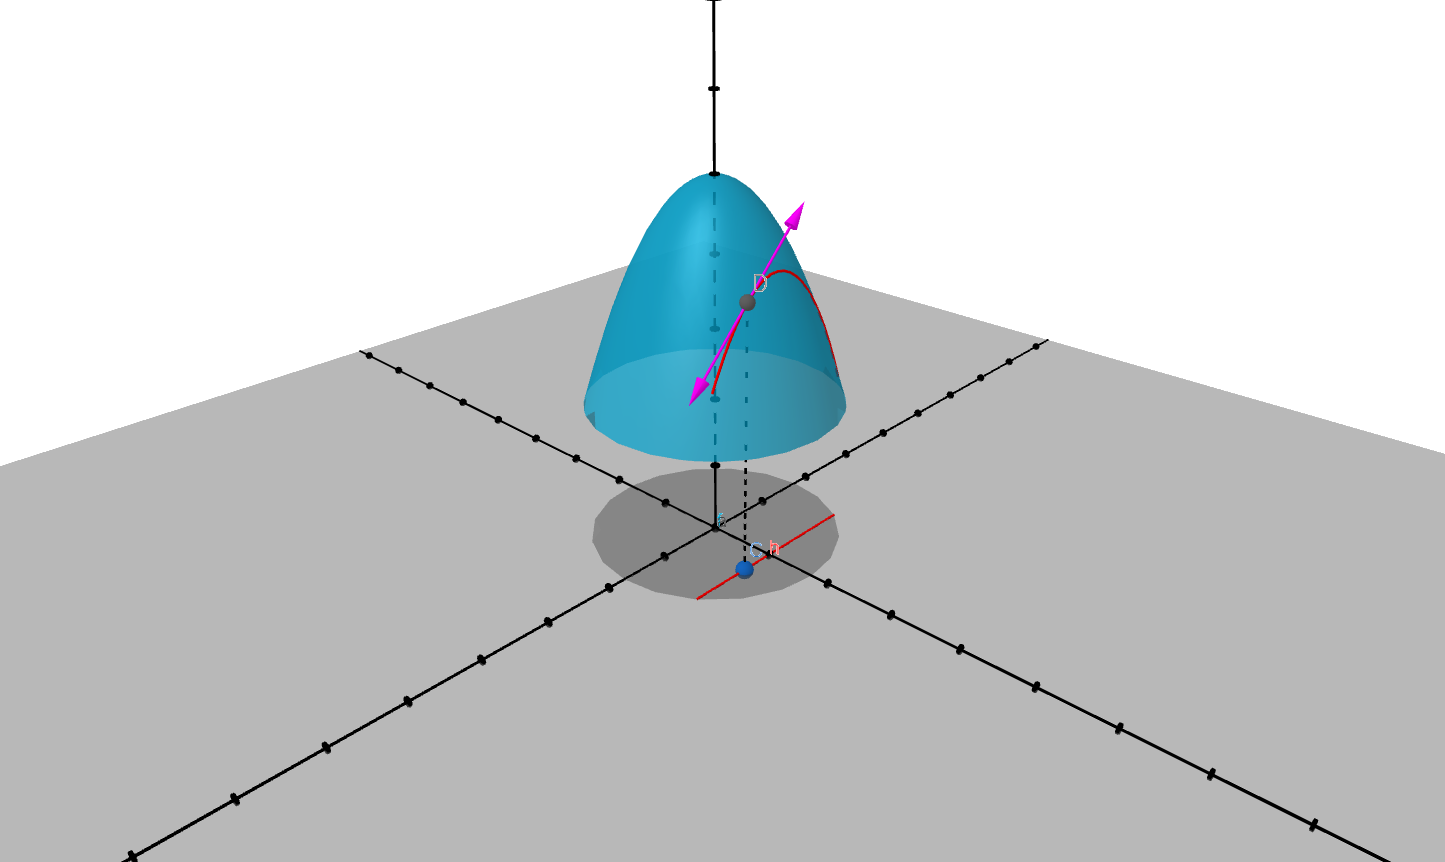
\includegraphics[scale=0.3]{diferencial1}
\end{center}

Para poner un ejemplo y en referencia al dibujo, consideramos $f(x,y) = -x^2-y^2+5$ restringida al conjunto de puntos $\{x^2+y^2 \leq 3\}$ que son la cónica azul y la sombra gris que proyecta en el suelo y el punto $x_0= \left(1,\frac{1}{2}\right)$ el punto azul de la sombra. Cuando fijamos la $y$ y tomamos la $x$ como variable libre nos estamos restringiendo a los puntos de la recta roja sobre el suelo, que son los que tienen como $y=\frac{1}{2}$ (la de $x_0$) y recorren $x$, cuyas imágenes forman la parábola roja en la cónica, que son los puntos de la forma $\left(x,\frac{1}{2}, f\left( x,\frac{1}{2}\right)\right)$. Si calculamos $\frac{\partial f}{\partial x} = -2x$, entonces vemos que el vector tangente a la gráfica en el punto $(1, \frac{1}{2}, \frac{15}{4})$, que es la imagen de $x_0$, es el vector formado por $\left(1, 0, \frac{\partial f}{\partial x}(x_0)\right) = \left(1, 0, -2\right)$.
\hrule
\begin{itemize}
\item Para seguir y poder calcular el hiperplano tangente a la gráfica en dicho punto hay que recordar una noción básica de Álgebra: un hiperplano viene dado por una forma lineal cuyos coeficientes pueden ser considerados como un vector, que será el vector ortogonal al hiperplano en cuestión llamado vector normal.
\item Por tanto, tenemos que calcular el vector normal a todos los vectores tangentes en cualquiera de las direcciones posibles. Como habíamos definido dichos vectores tangentes como:
$$v_j = \left(0, \cdots, \underbrace{1}_{j}, \cdots, 0, \frac{\partial f}{\partial x_j}(x_0)\right)$$
Si tomamos el vector
$$u = \left(\underbrace{\frac{\partial f}{\partial x_1}(x_0),\cdots, \frac{\partial f}{\partial x_n}(x_0)}_{\nabla f(x_0)}, -1 \right)$$
Entonces el producto escalar resulta como
$$v_j\cdot u = 0 + \cdots + \frac{\partial f}{\partial x_j}(x_0) + \cdots + 0 - \frac{\partial f}{\partial x_j}(x_0)$$
Luego es ortogonal a todos los demás vectores
\end{itemize}
A partir de aquí, $x\in \mathbb{R}^n$ denota un vector de dimensión $n$, no la coordenada $x$ del vector. De modo análogo, $z, f(x_0)\in \mathbb R$ se refieren a la coordenada $x_{n+1}$ del vector y del punto $x_0$ respectivamente.
\begin{itemize}
\item Los puntos que definen la variedad afín (el hiperplano tangente) que estamos buscando están definidos por los vectores $(x-x_0, z-f(x_0))\in \mathbb{R}^n$ donde además $(x-x_0, z-f(x_0))\cdot (\nabla f(x_0), -1) = 0$ porque tienen que ser perpendiculares al vector normal, por tanto:
$$z=\nabla f (x_0)(x-x_0)+ f(x_0)$$
Ecuación que nos resulta muy similar a la de la recta tangente en $\mathbb{R}^2$.

\item Para expresarlo en forma de forma lineal, basta con despejar $(\nabla f(x_0), -1)$ del producto escalar inicial, es decir:
$$(x,z)\cdot \underbrace{(\nabla f(x_0), -1)}_{L_{x_0}} = (x_0, f(x_0))\cdot (\nabla f(x_0), -1)$$
Luego los coeficientes de la forma lineal, son justamente los del vector normal. Para visualizarlo mejor, en caso de encontrarse en dimensión 3, tendríamos que:
$$(x,y,z)\cdot \left(\frac{\partial f}{\partial x}(x_1,x_2), \frac{\partial f}{\partial y}(x_1,x_2), -1,\right) = (x_1, x_2, f(x_1,x_2))\cdot \left(\frac{\partial f}{\partial x}(x_1,x_2), \frac{\partial f}{\partial y}(x_1,x_2), -1\right)$$
Donde $x,y,z\in \mathbb{R}$ denotan coordenadas y $x_1, x_2, x_3\in \mathbb{R}$ denotan las coordenadas del punto $x_0$ en cuestión.
\end{itemize}
\hrule
Para completar el ejemplo anterior, el vector normal $(\nabla f(x_0), -1)= (-2,-1,-1)$ que hemos tomado en positivo y el hiperplano tangente vendría dado por:
$$(x,y,z)\cdot \begin{pmatrix} 2 \\ 1 \\ 1\end{pmatrix} = \left(1,\frac{1}{2}, \frac{15}{4}\right)\cdot \begin{pmatrix} 2 \\ 1 \\ 1\end{pmatrix}$$

\begin{center}
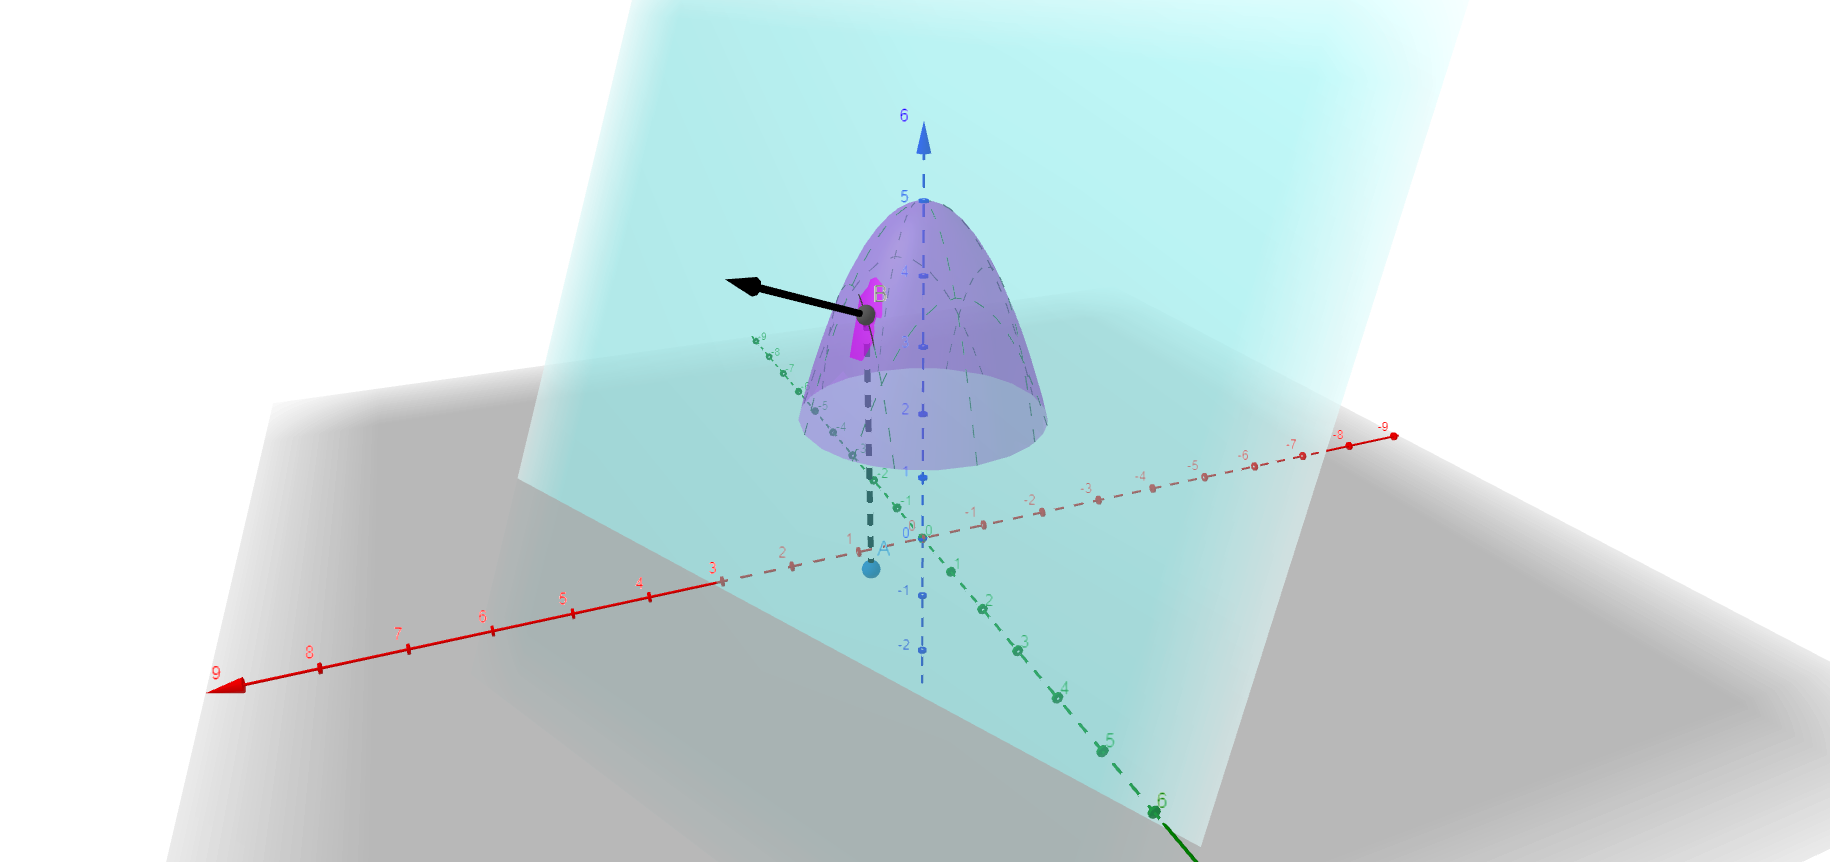
\includegraphics[scale=0.21]{diferencial2}
\end{center}
\hrule

\begin{theo}
Sea $f: A \subset \mathbb{R}^n \to \mathbb{R}$ diferenciable en $x_0 \in A$, entonces $f$ es continua en $x_0$.
\end{theo}
\begin{demo}
Sea $\varepsilon = 1$ existe $\delta' > 0$ de modo que $|| x - x_0 || < \delta' \Rightarrow |f(x) - f(x_0) - d f(x_0) (x - x_0)| < || x - x_0 ||$ por ser diferenciable. De este modo:
$$|f(x) - f(x_0)| \leq |f(x) - f(x_0) - df(x_0)\cdot (x - x_0)| + |df(x_0) \cdot (x - x_0)| \leq ||x-x_0|| \cdot (1 + || \nabla f(x_0) ||)$$
Luego, para cualquier $\varepsilon > 0$ arbitrario, tomando como $\delta = \min\left\lbrace \frac{\delta'}{||\nabla f || + 1}, \frac{\varepsilon}{1 + || \nabla f||}\right\rbrace$, obtenemos que $|f(x) - f(x_0)| < \varepsilon$ para $||x - x_0|| < \delta$.
\end{demo}

\underline{Ejemplo}

Sea $f(x,y) = \begin{cases} \frac{xy^2}{x^2 + y^4} & (x,y) \neq (0,0) \\ 0 & (x,y) = (0,0) \end{cases}$ para ver que no es continua veamos que no es diferenciable en el $(0,0)$.

Tomamos un vector unitario de dirección arbitraria $v = (\cos\theta , \sen\theta)$, entonces resulta :
$$\lim_{t\rightarrow 0}\frac{f((0,0) + tv) - f(0,0) -}{t}=\lim_{t\rightarrow 0} \frac{f(t\cos\theta, t \sen\theta)}{t} =\lim_{t\rightarrow 0} \frac{1}{t} \cdot \frac{t^3 \cos\theta \sen^2 \theta}{t^2 \cos^2 \theta + t^4 \sen^4 \theta}$$
Basta ahora con distinguir casos para evaluar la continuidad:
	\begin{itemize}
		\item $\cos\theta = 0$:
		$$\frac{1}{t} \cdot \frac{t^3 \cos\theta \sen^2 \theta}{t^2 \cos^2 \theta + t^4 \sen^4 \theta} \xrightarrow[t \to 0]{} 0 = D_v f(0,0)$$
		\item $\cos\theta \neq 0$:
		$$\frac{\cos\theta \sen^2\theta}{\cos^2 \theta + t^2 \sen^4 \theta} \xrightarrow[t \to 0]{} \frac{\sen^2 \theta}{\cos\theta} = D_v f(0,0)$$
\end{itemize}

Entonces, $f$ no es continua en $(0,0)$. También podíamos verlo por la aproximación por la curva $(y^2,y)\Rightarrow f(y^2, y) = \frac{y^4}{y^4 + y^4} = \frac{1}{2} \Rightarrow \nexists \lim_{(x,y) \to (0,0)} f(x,y)$.

\begin{prop}[Operaciones con Diferencibilidad]
Sean $f,g: A \subset \mathbb{R}^n \to \mathbb{R}$ y $x_0 \in A$. Si $f,g$ son diferenciables en $x_0$, entonces se cumple:
\begin{itemize}
\item $f + g$ es diferenciable y $d(f + g)(x_0) = d f (x_0)  + d g (x_0)$
\item $f \cdot g$ es diferenciable en $x_0$ y $d(f \cdot g)(x_0) = df(x_0) \cdot g(x_0) + f(x_0) \cdot dg(x_0)$
\item Si $f(x_0) \neq 0$, entonces $\frac{1}{f}$ es diferenciable en $x_0$ y $d \left( \frac{f}{g} \right) (x_0) = \frac{f(x_0) \cdot d g(x_0) - g(x_0) \cdot d f(x_0)}{f^2(x_0)}$
\end{itemize}
\end{prop}

\begin{theo}
Sea $f: A \subset \mathbb{R}^n \rightarrow \mathbb{R}$ y $x_0 \in A$. Si $\forall j \in \{1, \cdots, n\}: \exists \frac{\partial f}{\partial x_j} (x)$ y son funciones continuas en $x_0$, entonces $f$ es diferenciable.
\end{theo}
\begin{demo}
Para la demostración vamos a suponer que $n = 2$, puesto que para más dimensión basta con extrapolar esta demostración a dicha dimensión.

Sean $(x,y) \in \mathbb{R}^2$ y $x_0 = (a,b) \in A$, entonces:
$$f(x,y) - f(a,b) = f(x,y) - f(a,y) + f(a,y) - f(a,b) = (f(x,y) - f(a,y)) + (f(a,y) - f(a,b)) = $$
Considerando en el primer paréntesis la $y$ fija, entonces por el Tª. V. M. se tiene que $\exists \mu \in (x,a)\cup (a,x)$ que verifica las condiciones de abajo. Además, si consideramos en el segundo paréntesis la función como una función sobre una variable; la $y$, entonces por el mismo teorema $\exists v \in (y,b)\cup (b,y)$ que verifica la iguadad de abajo: 
$$=\left(\frac{\partial f}{\partial x} (\mu, y)\right) \cdot (x-a) + \left(\frac{\partial f}{\partial y} (a, \nu)\right) \cdot (y-b)$$
Veamos ahora la siguiente expresión:
$$|f(x,y) - f(a,b) - \nabla f(a,b) \cdot (x-a, y - b)| \leq \left|\frac{\partial f}{\partial x} (\mu, y) - \frac{\partial f}{\partial x} (a,b)\right| \cdot |x-a| + \left|\frac{\partial f}{\partial y} (a, \nu) - \frac{\partial f}{\partial y} (a,b)\right| \cdot |y-b|$$
Como las derivadas parciales son funciones continuas sobre $\mathbb{R}$, entonces:
$$\forall \varepsilon > 0, \ \exists \delta > 0 : ||(x-a, y-b)|| < \delta \Rightarrow \left|\frac{\partial f}{\partial x} (x, y) - \frac{\partial f}{\partial x} (a,b)\right| <  \frac{\varepsilon}{2} \mbox{ y } \left|\frac{\partial f}{\partial y} (x, y) - \frac{\partial f}{\partial y} (a,b)\right| <  \frac{\varepsilon}{2}$$
Luego los valores absolutos de las parciales los tenemos acotados y como los términos $|x-a|$ e $|y-a|$ al dividirse por la norma $||(x-a, y-b)||$ son menores o iguales que 1, tenemos que:
$$\frac{|f(x,y) - f(a,b) - \nabla f(a,b) \cdot (x-a, y - b)|}{||(x-a, y-b) ||} \leq \frac{\varepsilon}{2} + \frac{\varepsilon}{2} = \varepsilon$$
\end{demo}

\begin{obs}
Del ejemplo anterior, deducimos que
$$C^{1)}\Rightarrow \mbox{Diferenciable} \Rightarrow \forall x_0 \in A: \exists \nabla f(x_0)$$
Pero de ahí no podemos deducir que la función diferencial (que es la función gradiente) sea una función continua:
$$f(x,y) = \begin{cases} x^2 \cdot \sen\left(\frac{1}{x}\right)  & x \neq 0 \\ 0 & x = 0 \end{cases} \Rightarrow \forall x_0\in \mathbb R^2: \exists\nabla f(x_0) \mbox{ y diferenciable en }(0,0)$$
Sin embargo, la función $\nabla f(x,y) = (\frac{\partial f}{\partial x}f(x,y), \frac{\partial f}{\partial y} f(x,y))$ no es una función continua en $\mathbb{R}^2 \to \mathbb{R}^2$.
\end{obs}

\begin{defi}[Matriz Jacobiana]
Sea $f : A \subset \mathbb{R}^n \to \mathbb{R}^m$, definimos el \textbf{Jacobiano de $F$ en $x_0 \in A$} a:
$$J_f (x_0) = df(x_0) = \begin{pmatrix} \nabla f_1(x_0) \\ \vdots \\ \nabla f_m (x_0)\end{pmatrix} = \left(\frac{\partial f_j}{\partial x_k}(x_1, \cdots , x_n)\right)_{\substack{1 <= j <= m \\ 1<= k <= n}} \in M_{m \times n}$$
De modo análogo, cuando el espacio de llegada es $\mathbb{R}$, llamamos  \textbf{Hessiano} de $f$ en $x_0$ a:
$$H_f (x_0) = \begin{pmatrix} D_{11} f(x_0) & \ldots & D_{1n}f(x_0) \\ \vdots & • & \vdots \\ D_{n1}f(x_0) & \ldots & D_{nn}f(x_0) \\
\end{pmatrix} = \left( \frac{\partial^2 f}{\partial x_i \partial x_j } (x_0)\right)_{1 \leq i,j \leq n}$$
\end{defi}

\underline{Ejemplos}
\begin{enumerate}
\item Sea $f(x,y) = (x^2 y , y^3 x, x+y)$, entonces el jacobiano queda como:
$$J_f (x,y) = \begin{pmatrix} 2xy & x^2 \\ y^3 & 3y^2 x  \\ 1 & 1  \\\end{pmatrix} \in M_{3 \times 2}$$
\item Sea $g(x,y) = x^2y$, entonces el hessiano queda como:
$$H_g (x,y) = \begin{pmatrix} 2y & 2x  \\ 2x & 0 \end{pmatrix}$$
\end{enumerate}


\begin{theo}[Regla de la Cadena]
Sea $f: A \subset \mathbb{R}^n \to \mathbb{R}^m$ una función diferenciable en $x_0 \in A$ y $g: B \subset \mathbb{R}^m \to \mathbb{R}^p$ de modo que $f(A) \subset B$ y diferenciable en $f(x_0)$, entonces $\left(g \circ f\right) : A \subset \mathbb{R}^n \to \mathbb{R}^p$ es diferenciable en $x_0 \in A$ y su diferencial se calcula como:
$$d(g \circ f)(x_0) = dg(f(x_0)) \cdot df(x_0)$$
\end{theo}

Tal y como hemos demostrado antes, la diferencial en el punto $x_0$ se corresponde con el valor del gradiente en dicho punto, luego tendremos que:
$$d(g \circ f)(x_0) = \left( \frac{\partial (g \circ f)_j}{\partial x_k} (x_0) \right)_{\substack{1 \leq j \leq p \\ 1 \leq k \leq n
}}\in M_{p \times n}$$
De hecho, como hemos definido la relación entre la diferencial de la composición y las diferenciales de las funciones que se componen, tenemos que cada coordenada de dicha matriz se calcula como:
$$\frac{\partial (g \circ f)_j}{\partial x_k} (x_0) = \sum_{l = \ell}^{m} \frac{\partial g_j}{\partial x_\ell} (f(x_0)) \cdot \frac{\partial f_\ell}{\partial x_k}(x_0)$$
Por ser la diferencial de la composición el producto de las matrices $dg(f(x_0))$ y $df(x_0)$.

\underline{Ejemplo}

Sean $f: \mathbb{R}^2 \to \mathbb{R}^2$ y $g: \mathbb{R}^2 \to \mathbb{R}^3$ definidas como:
$$\begin{cases} f(x,y) = (x^2 y^3, xy) \\ g(a,b) = (ab, a^2, b^2)\end{cases}$$
Por tanto, la composición $g \circ f: \mathbb{R}^2 \to \mathbb{R}^3$
se definirá como:
$$\left(g\circ f \right)(x,y) = (x^3y^4, x^4y^6,x^2y^2)$$
La matriz del gradiente de la composición puede ser calculada fácilmente por el método explicado en secciones anteriores:
$$d(g \circ f) (x,y) = \begin{pmatrix} 3x^2y^4 & 4x^3y^3  \\ 4x^3y^6 & 6x^4y^5  \\ 2xy^2 & 2x^2y \\\end{pmatrix}$$
Sin embargo, podemos comprobar que el producto de matrices de las diferenciales correspondiente tiene como resultado dicha matriz:
\begin{align*}
d g (f(x,y)) = \begin{pmatrix}
xy & x^2 y^3 \\ 2x^2y^3 & 0 \\ 0 & 2xy
\end{pmatrix} & &
df(x,y) = \begin{pmatrix}
2x^3 & 3x^2y^2 \\ y & x
\end{pmatrix}
\end{align*}

$$d g (f(x,y)) \cdot df(x,y) = \begin{pmatrix}
xy & x^2 y^3 \\ 2x^2y^3 & 0 \\ 0 & 2xy
\end{pmatrix} \cdot  \begin{pmatrix}
2x^3 & 3x^2y^2 \\ y & x
\end{pmatrix} = \begin{pmatrix}
3x^2y^4 & 4x^3y^3 \\ 4x^3y^6 & 6x^4y^5 \\ 2xy^2 & 2x^2y
\end{pmatrix}$$

\underline{Ejemplo}

Sea $f: A \subset \mathbb{R}^n \to \mathbb{R}$ diferenciable podemos demostrar el cálculo de $d(f^2)(x)$ gracias a la regla de la Cadena.
Si consideramos $h: \mathbb{R} \to \mathbb{R}$ definida como $h(x)=x^2$, sabemos que $dh(x) = 2x$, luego:
$$d(f^2)(x) = d(h \circ f)(x) = d h(f(x)) \cdot df(x) = 2 f(x) \cdot df(x)$$
Gracias a un resultado como este podríamos demostrar la fórmula de la diferencial de un producto porque $f(x)\cdot g(x) = \frac{1}{4} [(f(x) + g(x))^2 - (f(x) - g(x))^2]$, luego basta con calcular:
$$d(f \cdot g) (x) = \frac{1}{4}\left[ 2 (f(x) + g(x)) \cdot (df(x) + dg(x)) - 2 (f(x) - g(x)) \cdot (d(f(x) - dg(x)) \right]$$
Que termina siendo la fórmula mencionada en secciones anteriores.

\subsection{Taylor, extremos y puntos críticos}
En este apartado, definimos los conceptos de extremos relativos, el nuevo punto silla y los puntos críticos. Asimismo, dejamos el terreno preparado para formular un Teorema Del Valor Medio en dimensión arbitraria y el esencial Teorema de Taylor. Por tanto, esta sección sienta las bases de la optimización y el cálculo analítico de la monotonía de las funciones estudiadas.

\begin{defi}[Conjunto convexo]
Sea $A \subset \mathbb{R}^n$, decimos que $A$ es \textbf{convexo} si 
$$\forall x,y \in A : L[x,y] = \left\lbrace tx + (1-t) y : 0 \leq t \leq 1 \right\rbrace \subset A$$
Donde la definición que se ha dado de $L[x,y]$ representa geométricamente el segmento que une ambos puntos.
\end{defi}
	    
\begin{obs}
Cuando manejábamos funciones de una variable tales como $f: I \subset \mathbb{R} \to \mathbb{R}$ derivable, podíamos afirmar que $\forall x,y \in I, \exists c \in L[x,y] : f(y) - f(x) = f'(c)(y-x)$ gracias al Teorema del Valor Medio. Sin embargo, en general es falso en el caso vectorial, por ejemplo sea $f: \mathbb{R} \to \mathbb{R}^2$ definida como $f(t)=(t^2, t^3)$ si tomamos $x = 0$ y $y=1$ podríamos suponer que:
$$(1,1) = f(1) - f(0) = df(c)(1-0) = df(c) : c \in [0,1]$$
Y, en realidad, vemos que el valor de la diferencial es:
$$df(c) = (2c,3c^2) = (1,1) \Leftrightarrow \begin{cases} c = \frac{1}{2} \\ c = \frac{1}{\sqrt{3}}\end{cases} \Rightarrow \#$$
\end{obs}
\newpage

\underline{Ejemplos}
    \begin{figure}[h]
    \centering
    
    \begin{subfigure}[h]{0.23\textwidth}
	\begin{tikzpicture}
    \draw[rotate=-45,fill=gray!30] (0,0) ellipse (30pt and 45pt);
    \end{tikzpicture}
    \caption{Conjunto Convexo}
    \end{subfigure}
    \hspace{2cm}
    \begin{subfigure}[h]{0.25\textwidth}
    \begin{tikzpicture}
    \draw[fill=gray!30] (0,0) to [out=140,in=90] (-1,-1)
    to [out=-90,in=240] (0.8,-0.6)
    to [out=60,in=-60] (1.2,1.2)
    to [out=120,in=90] (0.3,0.7)
    to [out=-90,in=20] (0.3,0)
    to [out=200,in=-40] (0,0);
    \draw (-0.5,-0.5) -- (0.7,0.7);
    \fill (-0.5,-0.5) circle[radius=1.5pt];
    \fill (0.7,0.7) circle[radius=1.5pt];
    \end{tikzpicture}
    \caption{Conjunto no Convexo}
    \end{subfigure}
	\end{figure}

\begin{lema}
Sea $f: A \subset \mathbb{R}^n \to \mathbb{R}^m$ diferenciable en el abierto $A$, entonces $\forall x,y \in A : L[x,y] \subset A$ y $\forall z \in \mathbb{R}^m$ se tiene que:
$$\exists c_z \in L [x,y] : \langle z, f(y) - f(x)\rangle = \langle z, df(c_z) \cdot (y-x) \rangle$$
\end{lema}
\begin{demo}
Al igual que hicimos con el Tª. V. M. en Análisis, vamos a definir una función auxiliar $\psi:[0,1] \to \mathbb{R}$ definida como $\psi(t) = \langle z, f(x+t(y-x)) \rangle$. Veamos ahora que:
$$\psi ' (t) = \frac{d}{dt}  \sum_{j=1}^{m} z_j \cdot f_j (x + t(y-x)) = \sum_{j=1}^{m} z_j \cdot \frac{d}{dt} f_j (x + t(y-x)) =$$
$$= \sum_{j=1}^{m} z_j \cdot d f_j (x + t(y-x)) \cdot (y-x)= \langle z, df(x + t(y-x)) \cdot (y-x) \rangle$$
Luego, como $\psi$ es derivable, entonces por el Teorema del Valor Medio se tiene que
$$\psi (1) - \psi (0) = \psi'(\alpha) (1-0) : \alpha \in (0,1)\Rightarrow \langle z, f(y) - f(x)\rangle = \langle z, df(x + \alpha (y-x)) \cdot(y-x) \rangle$$
Y vemos que basta llamar $x + \alpha (y-x) = c_z = \alpha y + (1 - \alpha ) x \in L[x,y]$.
\end{demo}


\begin{coro}
Sea $f: A \subset \mathbb{R}^n \to \mathbb{R}$ diferenciable en el abierto $A$, si $L[x,y] \subset A$, entonces se cumple la igualdad:
$$\exists c \in L[x,y] : f(y) - f(x) = df(c) \cdot (y-x)$$
\end{coro}
\begin{demo}
En el lema anterior, basta coger $z = 1$
\end{demo}

\begin{defi}[Norma de una aplicación lineal]
Sea $h: \mathbb{R}^n \to \mathbb{R}^m$ lineal definimos \textbf{la norma de h} como:
$$||h|| = \sup_{x \in \mathbb{R}^n \setminus \{0\}} = \frac{||h(x)||}{||x||} = \sup_{||y|| = 1} || h(y)|| $$
La última igualdad se da porque como el denominador es un escalar, puede entrar dentro de la norma del numerador y por ser $h(x)$ lineal, finalmente se tiene que $\left|\left|h\left(\frac{x}{||x||}\right)\right|\right|$, es decir, que se reduce al supremo de las imágenes de vectores unitarios.
\end{defi}

\begin{obs}
Es un buen ejercicio probar que el espacio de matrices $(M_{m \times n}, || \cdot || ) $ con la norma definida anteriormente es un espacio normado.
\end{obs}

\begin{theo}[Teorema de los incrementos finitos]
Sea $f: A \subset \mathbb{R}^n \to \mathbb{R}^m$ diferenciable en el abierto $A$, si $L[x,y] \subset A$, se satisface que:
$$|| f(y) - f(x) || \leq \sup _{c \in L[x,y]} || df(c) || \cdot || y - x||$$
\end{theo}

\begin{demo}
Si  $f(x) = f(y)$ se cumple trivialmente, así que vamos a suponer que $f(x) \neq f(y)$. Sea $z = \frac{f(y) - f(x)}{|| f(y) - f(x) ||} \in \mathbb{R}^m$, por el lema anterior:
$$\exists c_z \in L[x,y] :  \langle z, f(y) - f(x)\rangle = \langle z, df(c_z) \cdot (y-x) \rangle$$
Sustituyendo $z$ en la expresión anterior:
$$\langle z, f(y) - f(x)\rangle = \left\langle \frac{f(y) - f(x)}{|| f(y) - f(x) ||}, f(y) - f(x)\right\rangle = \frac{1}{|| f(y) - f(x) ||} \langle f(y) - f(x), f(y) - f(x) \rangle =$$
$$=\frac{1}{|| f(y) - f(x) ||} \cdot || f(y) - f(x) ||^2 = || f(y) - f(x) ||$$

Por la desigualdad de Cauchy - Schwarz 
$$|| f(y) - f(x) || \leq 1 \cdot || df(c_z) \cdot (y-x) || \leq || df(c_z) || \cdot ||y-x|| \leq sup_{c \in L[x,y]} || df(c)|| \cdot || y - x|| $$
\end{demo}

\begin{coro}
Si $f: A \subset \mathbb{R}^n \to \mathbb{R}^m$, donde $A$ es convexo y abierto, es diferenciable y $df = 0$ en $A$, entonces $f$ es constante.
\end{coro}
\begin{demo}
Sean $x,x_0 \in A$, por la convexidad de $A$, $L[x,x_0] \subset A$ y, por el Teorema de los Incrementos Finitos, se tiene que:
$$|| f(x) - f(x_0) || \leq \sup_{c \in L[x,x_0]} || d f(c) || \cdot || x - x_0 || = 0 \Rightarrow f(x) = f(x_0)$$
\end{demo}

\begin{defi}[Derivada Segunda]
Sea $f: A \subset \mathbb{R}^n \to \mathbb{R}^m$ donde $A$ es abierto y $u,v \in \mathbb{R}^n$. La \textbf{derivada segunda} de $F$ se define\footnote{Nótese que el orden de la derivación parcial es de dentro hacia fuera, comenzando por la variable más a la derecha} (siempre que existan) como: 
$$D_{u,v} = D_u (D_v f)$$
Si tomamos como vectores los canónicos $u = e_i, v = e_j$, entonces:
$$D_{e_i, e_j} f = D_{i,j} f = \frac{\partial^2 f}{\partial x_i \partial x_j} = f_{ij} = f_{x_i x_j}$$
Y si además lo hacemos sobre el mismo vector en cada iteración:
$$\frac{\partial^2 f}{\partial x_i^2} = f_{ii} = f_{x_i x_i}$$\\
De manera análoga, se definen las derivadas de cualquier orden.
$$D_{i_k, \ldots, i_1} f = \frac{\partial^k f}{\partial x_{i_k} \ldots \partial x_{i_1}} : i_1, \ldots, i_k \in \{1, \ldots, n\}$$
\end{defi}

\underline{Ejemplo}

Sea $f(x,y)= yx^2 + xy^3$
\begin{align*}
\frac{\partial f}{\partial x} & = 2xy + y^3 & \frac{\partial f}{\partial y} & = x^2 + 3xy^2 & \frac{\partial^2 f}{\partial x^2} & = 2y \\ \frac{\partial^2 f}{\partial y^2} & = 6xy & \frac{\partial^2 f}{\partial y \partial x} & = 2x + 3y^2 & \frac{\partial^2 f}{ \partial x\partial y} & = 2x + 3y^2
\end{align*}

\begin{defi}[Función de Clase k]
Se dice que $f$ es \textbf{función de clase k} y se denota por $f \in \mathcal{C}^{k)} (A)$ con $A \subset \mathbb{R}^n$ abierto, si $\forall \{i_1, \ldots, i_k\} \subset \{1, \ldots, n\}: \exists D_{i_k, \ldots, i_1} f$ y todas son funciones continuas.
\end{defi}

\begin{theo}[de Schwarz - Clairaut]
Sea $f \in \mathcal{C}^{2)} (A)$ donde $A \subset \mathbb{R}^n$ es abierto, entonces $\forall i,j \in \{1, \ldots, n\}$ se cumple que: 
$$\frac{\partial^2 f}{\partial x_i \partial x_j} = \frac{\partial^2 f}{\partial x_j \partial x_i}$$
Es decir, las derivadas ``cruzadas'' coinciden (la diagonal de derecha a izquierda en la matriz de la diferencial).
\end{theo}
\begin{demo}
Podemos suponer que $n = 2$ y $m = 1$ porque por inducción se puede hacer extensible para $n$. Además si $m> 1$, entonces al tener que hacerlo sobre cada componente y unir en un vector los resultados se tiene trivialmente por haberlo demostrado para $m=1$. Considerando $(x,y)\in A$ y $h,k\in \mathbb R$ definimos las siguientes funciones:
\begin{align*}
g_k(u)=f(u,y+k)-f(u, y) && j_h(u) = f(x +h,u) - f(x, u)
\end{align*}
Y determinamos el siguiente conjunto:
$$A_{h,k} = f(x+h, y+k) - f(x+h, y) - f(x,y+k) + f(x,y) \Rightarrow \begin{cases} A_{h,k} = g_k(x+h) - g_k (x) \\ A_{h,k} = j_{h}(y+k) - j_h(y) \end{cases}$$
Por hipótesis, la función $g_k$ es continua y derivable por serlo $f$ y ser suma y composición de $f$ y funciones continuas, luego por el Teorema del Valor Medio, tenemos $c_{h,k}\in (x, x+h)$ y $d_{h,k}\in (y, y+k)$ (en caso de ser negativo se da la vuelta a los intervalos) tal que:
$$g_k(x+h) - g_k (x) = g'_k(c_{h,k}) \cdot (h-0) = \left( \frac{\partial f}{\partial x}\left(c_{h,k}, y+k\right) - \frac{\partial f}{\partial x}\left(c_{h,k}, y\right)\right) \cdot h = \frac{\partial^{2}f}{\partial y \partial x}\left(c_{h,k}, d_{h,k}\right) \cdot h \cdot k$$
En concreto, la última igualdad viene de considerar la función $\frac{\partial f}{\partial x}(c_{h,k}, y)$ como una función (continua y derivable por ser $f\in C^{2)}(A)$) sobre la variable $y$ y aplicar también el teorema del valor medio para la misma.

De este modo, si consideramos el mismo razonamiento sobre la función $j_h(u)$, tenemos $c'_{h,k}\in (x, x+h)$ y $d'_{h,k}\in (y, y+k)$ tal que:
$$j_h(y+k) - j_h (y) = j'_h(d'_{h,k}) \cdot (k-0) = \left( \frac{\partial f}{\partial y}\left(x + h, d'_{h,k}\right) - \frac{\partial f}{\partial y}\left(x+h, d'_{h,k}\right)\right) \cdot k = \frac{\partial^{2}f}{\partial x \partial y}\left(c'_{h,k}, d'_{h,k}\right) \cdot h \cdot k$$
Luego, como ambas cosas son iguales a $A_{h,k}$, se tiene que:
$$\frac{\partial^{2}f}{\partial x \partial y}\left(c'_{h,k}, d'_{h,k}\right) \cdot \cancel{h} \cdot \cancel{k} = \frac{\partial^{2}f}{\partial y \partial x}\left(c_{h,k}, d_{h,k}\right) \cdot \cancel{h} \cdot \cancel{k} \xrightarrow[k\rightarrow 0]{h\rightarrow 0} \frac{\partial^{2}f}{\partial x \partial y}\left(x,y \right)= \frac{\partial^{2}f}{\partial y \partial x}\left( x,y\right) $$
Y, en particular, cuando pasamos al límite en el último paso, podemos afirmar la igualdad porque $f\in C^{2)}(A)$ ya que como $c_{h,k}$ y $d_{h,k}$ se aproximan a los valores de $x$ e $y$, la función toma el mismo valor en el límite que en la imagen a consecuencia de la continuidad que le confiere $f\in C^{2)}(A)$.
\end{demo}

\begin{obs}
En general, la igualdad no es cierta si $f \notin \mathcal{C}^{2)} (A)$. Por ejemplo, $f(x,y) = \begin{cases} \frac{xy^3}{x^2 + y^2} & (x,y) \neq (0,0) \\ 0 & (x,y) = (0,0) \end{cases}$. $f$ tiene derivadas de orden 2 en $\mathbb{R}^n$ y $\frac{\partial^2 f }{\partial x \partial y} (0,0) \neq \frac{\partial^2 f }{ \partial y\partial x} (0,0)$.
\end{obs}

\begin{coro}
Si $f \in \mathcal{C}^{k)} (A)$ es de clase $k$ y $\sigma \in \mathcal{S}_k$ es el conjunto de permutaciones de $\{1, \ldots, k\}$, entonces 
$$D_{i_1, \ldots, i_k} f = D_{\sigma (\{1, \ldots, k\})} f$$
Es decir, el orden de derivación sobre cada dirección no influye en el resultado final.
\end{coro}

\begin{theo}[Teorema de Taylor]
Sea $f: A \subset \mathbb{R}^n \to \mathbb{R}$ donde $A$ es abierto y $f\in \mathcal{C}^{k+1)} (A)$. Si tomamos dos puntos $x_0 \in A$ y $h \in \mathbb{R}^n \setminus \{0\}$ de modo que $L[x_0,x_0 + h] \subset A$, entonces $\exists c \in L[x_0, x_0 + h]$ tal que:
$$f(x_0 + h) = f(x_0) + \sum_{i_1=1}^{n} D_{i_1} f(x_0) \cdot h_{i_1} + \frac{1}{2} \sum_{\substack{i_1 = 1 \\ i_2 = 1}}^{n} D_{i_1, i_2} f(x_0) \cdot h_{i_1} \cdot h_{i_2} + \cdots$$
$$\cdots + \frac{1}{k!} \sum_{\substack{i_1 = 1 \\ \cdots \\ i_k = 1}}^{n} D_{i_1, \ldots, i_k} f(x_0) \cdot h_{i_1} \cdot \ldots \cdot h_{i_k} + \frac{1}{(k+1)!} \sum_{\substack{i_1 = 1 \\ \cdots \\ i_{k+1} = 1}}^{n} D_{i_1, \ldots, i_{k+1}} f(c) \cdot h_{i_1} \cdot \ldots \cdot h_{i_{k+1}}$$
\end{theo}

\underline{Ejemplo}

Sea $f(x,y) = x^2 - 2y^2 + 4xy - 3$, calculemos el Polinomio de Taylor de orden 2 en el punto $(1,1) \in \mathbb{R}^2$. Observamos que por la definición que se ha dado, el polinomio de Taylor de orden dos se puede expresar como:
$$\begin{cases} \nabla f(x,y) = (2x + 4y, -4y + 4x) \\ H_f (x,y) =\begin{pmatrix} 2 & 4 \\ 4 & -4 \end{pmatrix} \\ h = (x,y) - (1,1) = (x-1, y-1) \end{cases} \Rightarrow P_2\left((x,y), x_0\right) = f(x_0) + \nabla f(x_0) \cdot h + h \cdot H_f(x_0) \cdot h^t$$
Luego, sustituyendo tenemos:
$$P_2((x,y); (1,1)) = 0 + \langle \overbrace{(6,0)}^{\nabla f(x_0)},(x-1, y-1) \rangle + \frac{1}{2} \cdot \begin{pmatrix}
x-1 & y-1
\end{pmatrix} \cdot \overbrace{\begin{pmatrix}
2 & 4 \\ 4 & -4
\end{pmatrix}}^{H_f(x_0)} \cdot \begin{pmatrix}
x-1 \\ y-1
\end{pmatrix} $$
$$= 6(x-1) + \frac{1}{2} \cdot \begin{pmatrix}
2(x-1) + 4 (y-1) & 4(x-1) - 4 (y-1)
\end{pmatrix}\cdot \begin{pmatrix}
x-1 \\ y-1
\end{pmatrix} $$
$$= 6(x-1) + \frac{1}{2} \left( 2 (x-1)^2 + 4 (x-1)(y-1) + 4 (x-1)(y-1) - 4 (y-1)^2 \right)$$
$$= x^2 - 2y^2 + 4xy - 3$$

\begin{defi}[Extremos y puntos críticos]
Sea $f: A \subset \mathbb{R}^n \to  \mathbb{R}$ y $x_0 \in A$, entonces:
\begin{itemize}
\item Decimos que $x_0$ es un \textbf{mínimo relativo} si $f(x) \geq f(x_0) : \forall x \in B(x_0, \varepsilon) \subset A$
\item Decimos que $x_0$ es un \textbf{mínimo relativo} si $f(x) \leq f(x_0) : \forall x \in B(x_0, \varepsilon) \subset A$
\item Decimos que un \textbf{extremo es absoluto} si la desigualdad correspondiente es cierta $\forall x \in A$
\item Decimos que $x_0$ es un \textbf{punto crítico} si $\nabla f(x_0) = 0$
\item Decimos que $x_0$ es un \textbf{punto silla} si es un punto crítico que no es un extremo relativo.
\end{itemize}
\end{defi}

\begin{theo}
Sea $f: A \subset \mathbb{R}^n \to \mathbb{R}$ donde $A$ es abierto y supuesto que existe $\nabla f(x_0)$. Si $x_0 \in A$ es un extremo relativo, entonces $\nabla f (x_0) = 0$.
\end{theo}

\begin{demo}
Sea $j \in \{1, \ldots, n\}$. Supongamos que $x_0$ es un máximo relativo (razonamos de forma análoga para el caso del mínimo relativo). Entonces
$$\frac{f(x_0 + t \cdot e_j) - f(x_0)}{t} = \begin{cases} \leq 0 & t> 0 \\ \geq 0 & t < 0 \end{cases}\Rightarrow \frac{\partial f}{\partial x_j} (x_0) = 0$$
\end{demo}

\begin{obs}
Si $f \in \mathcal{C}^{2)}(A), x_0$, definimos el Hessiano como $ H_f (x_0) = \begin{pmatrix}
\frac{\partial^2 f}{\partial x_j \partial x_k}
\end{pmatrix}_{1 \leq j,k \leq n}$, es decir, es una matriz cuadrada simétrica. Si recordamos del curso de Álgebra Lineal, definíamos las formas cuadráticas como las aplicaciones $Q \in M_{n \times n}$ tales que
\begin{align*}
Q: \mathbb{R}^n &\to \mathbb{R} \\ x &\mapsto Q(x) = x Q x^t
\end{align*}
Es decir, los Hessianos son formas cuadráticas.
\end{obs}

\begin{defi}[Forma cuadrática]
Una forma cuadrática $Q \in M_{n \times n}$ se denomina:
\begin{itemize}
\item Definida positiva si $Q(x) > 0 : \forall x \in \mathbb{R}^n \setminus \{0\}$
\item Definida negativa si $Q(x) < 0 : \forall x \in \mathbb{R}^n \setminus \{0\}$
\item Semidefinida positiva si $Q(x) \geq 0 : \forall x \in \mathbb{R}^n$
\item Semidefinida negativa si $Q(x) \leq 0 : \forall x \in \mathbb{R}^n$
\end{itemize}
\end{defi}

\begin{theo}[Caracterización de los puntos críticos vía Hessiano]
Sea $f \in \mathcal{C}^{2)} (A)$ con $A \subset \mathbb{R}^n$, $x_0 \in A$ y $\nabla f(x_0) = 0$, se tiene que:
\begin{itemize}
\item Si $H_f (x_0)$ es definida negativa, entonces $x_0$ es un máximo relativo.
\item  Si $H_f (x_0)$ es definida positiva, entonces $x_0$ es un mínimo relativo.
\item  Si $x_0$ es un máximo relativo, entonces $H_f (x_0)$ es semidefinida negativa.
\item   Si $x_0$ es un mínimo relativo, entonces $H_f (x_0)$ es semidefinida positiva.
\item  Si $H_f (x_0)$ es indefinida, entonces $x_0$ es un punto silla.
\end{itemize}
\end{theo}

\begin{demo}
Se muestra la demostración del primer apartado solo, puesto que las demás son completamente análogas a la que siguen.

Sea $S = \{x \in \mathbb{R}^n : || x || = 1\}$ compacto de $\mathbb{R}^n$, como la aplicación $H_f (x_0) = Q_{x_0} : \mathbb{R}^n \to \mathbb{R}$ es continua, alcanza un máximo y mínimo en $S$. Además, como $Q$ es definida negativa, por hipótesis se tiene que:
$$\exists \tilde{x}=\max\{H_f(x_0)(x)\} \in S : 0 > Q(\tilde{x}) \geq Q(x) : \forall x \in S$$
Sea $-\varepsilon_0 = Q(\tilde{x})$ y teniendo en cuenta a la continuidad de las derivadas parciales de segundo orden de $f$, se tiene que: 
$$\mbox{ Dado } \varepsilon_0 > 0, \exists \delta > 0 : || x - x_0 || < \delta \Rightarrow \left| D_{ij} f(x) - D_{ij} f(x_0) \right| < \frac{\varepsilon_0}{2n^2} : \forall i,j = 1, \ldots, n$$
Por otra parte, si $h \in \mathbb{R}^n$ no nulo, se verifica que:
$$Q(h)= || h||^2 \cdot Q\left(\frac{h}{||h||}\right) \leq ||h||^2 \cdot  Q(\tilde{x}) = -\varepsilon_0 \cdot ||h||^2$$
Por el Teorema de Taylor, $\exists c \in L[x_0, x_0 + h]$ de forma que para $||h|| < \delta$ ocurre:
$$f(x_0 + h) - f(x_0) = \frac{1}{2} \cdot h \cdot H_f(c) \cdot h^t = \frac{1}{2} \sum_{\substack{i = 1 \\ j = 1}}^{n} D_{ij} f(c) \cdot h_i \cdot h_j $$
$$= \frac{1}{2} \left[ \left(\sum_{\substack{i = 1 \\ j = 1}}^{n} D_{ij} f(c) - D_{ij} f(x_0)  \right) \cdot h_i \cdot h_j + \underbrace{\sum_{\substack{i = 1 \\ j = 1}}^{n} D_{ij} f(x_0) \cdot h_i \cdot h_j}_{Q(h)} \right] \leq \frac{1}{2} \left[ n^2 \frac{\varepsilon}{2n^2} \cdot ||h||^2 - ||h||^2 \varepsilon_0 \right] < 0$$
El resto de apartados se demuestran de forma análoga.
\end{demo}

\begin{obs}
Sea $f : A \subset \mathbb{R}^2 \to \mathbb{R}\in \mathcal{C}^{2)}(A)$ con $A$ abierto y $(x_0, y_0) \in A$, entonces el Hessiano es de la forma:
$$H_f (x_0, y_0) = \begin{pmatrix} \frac{\partial^2 f}{\partial x^2} (x_0, y_0) & \frac{\partial^2 f}{\partial x \partial y} (x_0, y_0) \\ \frac{\partial^2 f}{\partial x \partial y} (x_0, y_0) & \frac{\partial^2 f}{\partial y^2} (x_0, y_0) \\ \end{pmatrix} = \begin{pmatrix} a & b \\ b & c \end{pmatrix}$$
Es decir, si denotamos al determinante Hessiano con $\Delta = det(H_f (x_0, y_0)) = ac - b^2$, entonces para si $h = (h_1, h_2) \in \mathbb{R}^2$, tenemos
$$h H_f (x_0, y_0) h^t = a \cdot h_1^2 + 2 b \cdot h_1 \cdot h_2 + c \cdot h_2^2$$
Lo que da lugar al siguiente teorema.
\end{obs}

\begin{theo}
Sea $\nabla f (x_0, y_0) = 0$, entonces considerando el determinante del Hessiano:
\begin{itemize}
\item $\Delta > 0 = \begin{cases} a > 0 & (x_0, y_0) \mbox{ mínimo relativo} \\ a < 0 & (x_0, y_0) \mbox{ máximo relativo}\end{cases}$
\item $\Delta < 0 \Rightarrow (x_0, y_0)$ es punto silla
\item $\Delta = 0$
\end{itemize}
En el fondo esto es extensible a dimensiones mayores que 2 utilizando los criterios del Álgebra Lineal para decidir cuando una forma cuadrática (el Hessiano) es definida positiva, definida negativa, etc.
\end{theo}

\begin{demo}
Demostraremos sólo el primer apartado puesto que los demás se basan en una demostración por casos como la que sigue.

Lo que queremos ver es que si $h \neq 0$, entonces $ah_1^2 + 2bh_1h_2 + ch_2^2 > 0$. Sabemos que, por hipótesis, $ac - b^2 > 0$ y que $a > 0$. La clave está en escribir $ah_1^2 + 2bh_1h_2 + ch_2^2 = a \left( h_1 + \frac{b}{a} h_2 \right)^2 + \frac{\Delta}{a} h_2^2$ donde dicha igualdad viene de:
$$ a \left( h_1 + \frac{b}{a} h_2 \right)^2 + \frac{\Delta}{a} h_2^2 = a \left( h_1^2 + \frac{b^2}{a^2} h_2^2 + 2 \cdot \frac{b}{a} h_1 h_2\right) + \left( c - \frac{b^2}{a} h_2^2 \right)$$
Gracias a las hipótesis de partida, tenemos que $ a \left( h_1 + \frac{b}{a} h_2 \right)^2 + \frac{\Delta}{a} h_2^2 >0 $ ya que, aunque podría darse que $ h_1 + \frac{b}{a} h_2 $ pueda anularse, el segundo término no.
\end{demo}
$$
\begin{tikzpicture}
\begin{axis}
\addplot3 [surf,shader=flat] {x^2-y^2};
\end{axis}
\put(95,74){\textbullet}
\end{tikzpicture}$$
$$\mbox{Ejemplo de Punto de Silla}$$
\underline{Ejemplo}

Estudia los puntos críticos de las siguiente función y determina si son máximos o mínimos locales:
$$f(x,y) = x^3 + y^3 - 3 \cdot a xy \Rightarrow \nabla f(x,y) = (3x^2 - 3ay, 3y^2 - 3ax)$$
\begin{itemize}
\item Supongamos $a \neq 0$, entonces igualando a 0 ambas componentes:
$$\begin{cases} 3x^2 - 3ay = 0 \\ 3y^2 - 3ax = 0 \end{cases} \Rightarrow\begin{cases} y = \frac{x^2}{a} \\ \frac{x^4}{a^2} - ax = 0 \Rightarrow x (x^3 - a^3) = 0  \end{cases} \Rightarrow \begin{cases} x = 0 & y = 0 \\ x = a & y =a \end{cases}$$
\item Si $a = 0$ trivialmente se tiene que sólo es punto crítico el $(0,0)$.
\item Si calculamos el determinante del Hessiano, tenemos que:
$$H_f (x,y) = \begin{pmatrix} 6x & -3a \\ -3a & 6y  \\ \end{pmatrix} \Rightarrow \Delta = 36 xy - 9 a^2$$

\item Si $a \neq 0$, tenemos que:
\begin{itemize}
\item $(0,0) \Rightarrow \Delta = -9a^2 < 0 \Rightarrow $ punto silla
\item $(a,a) \Rightarrow \Delta = 27a^2 > 0 \Rightarrow \begin{cases} a > 0 & \mbox{ mínimo relativo} \\ a < 0 & \mbox{ máximo relativo} \end{cases}$
\end{itemize}

\item Si $a = 0$, entonces $\Delta = 0$, así que no podemos deducir nada de ello. Es necesario \textbf{calcularlo a mano} y finalmente sale $f(0,0) = 0$.
completar
\end{itemize}

\chapter{TEOREMAS NOTABLES}
En este capítulo vamos a enunciar y demostrar tres resultados fundamentales para otros ámbitos de las matemáticas como son las ecuaciones en derivadas parciales o las ecuaciones algebraicas. Su estudio nace de la necesidad de poder operar y trabajar con funciones como si de números se tratase para poder realizar operaciones como dividir (multiplicar por el inverso) o poder expresar dicha función de una forma más conveniente.

\section{TEOREMA DE LA FUNCIÓN INVERSA}
Nuestro objetivo ahora es dada $f : A \subset \mathbb{R}^n \to \mathbb{R}^n$, cuándo y de qué forma podemos encontrar la solución:
$$ f(x) = y : \begin{cases} f_1 (x_1,…,x_n )=y_1 \\ \vdots \\ f_n (x_1,…,x_n )=y_n \end{cases}$$
Cuando trabajamos en $\mathbb{R}$, si tenemos $f : I \subset \mathbb{R} \to \mathbb{R}$ de forma que $f \in \mathcal{C}^{1)}$ y $x_0 \in I$ un punto donde la derivada no se anula $f'(x_0) \neq 0$, entonces $f$ es estrictamente monótona en un entorno de $x_0$ y, por lo tanto, invertible en un entorno de $x_0 \in I$. Además, si $g=f^{-1}$ sabemos calcular la derivada: 
$$g' (f(x)) = \frac{1}{f'(x)}$$
Luego, con este teorema pretendemos hacer extensible dicha demostración a dimensión arbitraria y como vimos que $df(x_0)$ jugaba el papel de $f'(x_0)$ será razonable pensar que la condición imprescindible será $\det (df(x_0)) \neq 0$.

\begin{defi}
Para las posteriores demostraciones y enunciados, vamos a definir dos objetos fundamentales a los que haremos referencia:
$$L_i (\mathbb{R}^n, \mathbb{R}^n) = \{M \in M_{n \times n} : \det (M) \neq 0\}$$
Es decir, las matrices cuadradas invertibles de orden $n$.
\begin{align*}
\mathcal{L}^{-1} : L_i (\mathbb{R}^n, \mathbb{R}^n) &\to L_i (\mathbb{R}^n, \mathbb{R}^n) \\ M &\mapsto \mathcal{L}^{-1} (M) = M^{-1}
\end{align*}
Es decir, la aplicación invertir matriz cuando sabemos que esta tiene inversa.
\end{defi}

\begin{obs}
Es importante ver que podemos identificar $M_{n \times n}$ con el espacio euclídeo $\mathbb{R}^{n^2}$, puesto que podemos realizar la siguiente asignación:
$$M = \begin{pmatrix}
a_{11} & \cdots & a_{1n} \\ \vdots & \ddots & \vdots \\ a_{n1} & \cdots & a_{nn}
\end{pmatrix} \longmapsto (a_{11}, \cdots, a_{1n} ,a_{21}, \cdots a_{2n}, \cdots, a_{n1}, \cdots, a_{nn})$$
Y de este modo, $L_i (\mathbb{R}^n, \mathbb{R}^n)$ se puede considerar como un subconjunto de $\mathbb{R}^{n^2}$, luego tiene sentido hablar de abiertos en dicho conjunto.
\end{obs}

\begin{lema}
El conjunto $L_i (\mathbb{R}^n, \mathbb{R}^n)$ es un abierto en $M_{n \times n} = \mathbb{R}^{n^2}$ y la aplicación $\mathcal{L}^{-1}$ es de clase $C^{\infty)}$.
\end{lema}

\begin{demo}
Sea $M \in L_i (\mathbb{R}^n, \mathbb{R}^n)$, por definición $\det (M) \neq 0$, es decir, $L_i (\mathbb{R}^n, \mathbb{R}^n) = d^{-1} (\mathbb{R} \setminus \{0\})$ donde $d$ es la aplicación $M \stackrel{d}{\longmapsto} \det(M)$. Trivialmente $\mathbb{R}\setminus{\{0\}}$ es un abierto y omo $d$ es una función continua por ser una combinación polinómica de las entradas de la matriz, la inversa del abierto $(\mathbb{R} \setminus \{0\})$ es abierto.

Análogamente vemos que $\mathcal{L}^{-1} \in \mathcal{C}^{\infty )} (L_i (\mathbb{R}^n, \mathbb{R}^n))$. Por ejemplo:
\begin{itemize}
\item Si $n = 1$, entonces $\mathcal{L}^{-1} (a) = \frac{1}{a} : a \neq 0$ y, por tanto, $\mathcal{L}^{-1} \in \mathcal{C}^{\infty )}$

\item Si $n = 2$ y definiendo $M = \begin{pmatrix} a & b \\ c & d \end{pmatrix}$, denotamos $\Delta = \det (M) = ad -  bc \neq 0$ así que:
$$\mathcal{L}^{-1} (M) = \begin{pmatrix} \frac{d}{\Delta} & \frac{-b} {\Delta} \\ \frac{-c}{\Delta} & \frac{a}{\Delta}\end{pmatrix}$$
es una función racional, lo que implica $\in \mathcal{C}^{\infty )} (L_i (\mathbb{R}^2, \mathbb{R}^2))$

\item Y de este modo, basta con ver como se trata el determinante en cada dimensión para poder hacerlo por inducción.
\end{itemize}
\end{demo}

\begin{lema}[Teorema del Punto Fijo]
Sea $(X, d)$ espacio métrico completo y sea $f : X \to X$ tal que:
$$\forall x,y \in X : d(f(x), f(y)) \leq k \cdot d(x,y) \mbox{ 	con } 0 < k <1$$
Es decir, $f$ es una contracción, entonces existe un único punto fijo:
$$\exists ! x \in X : f(x) = x$$
\end{lema}
\begin{demo}
Sea $x_1 \in X$ y $x_{n+1} = f(x_n)$, en primer lugar probaremos que es de Cauchy. Sea $n \geq 2$, tenemos que:
$$d(x_{n+1}, x_n) = d(f(x_n), f(x_{n-1})) \leq k \cdot d(x_n, x_{n-1}) \leq k^2 \cdot d(x_{n-1}, x_{n-1}) \leq \ldots \leq k^{n-1} d(x_2, x_1)$$ 
Ahora, si tomamos $m > n \geq 1$, ocurre que:
$$d(x_m, x_n) \leq d(x_m, x_{m-1}) + d(x_{m-1}, x_{m-2}) + \ldots + d(x_{n+1}, x_n) \leq (k^{m-2} + \ldots + k^{n-1}) \cdot d(x_2, x_1)$$
$$= \frac{k^{n-1} - k^{m-1}}{1 - k} \cdot d(x_2, x_1) \xrightarrow[m,n \to \infty]{} 0$$
Por completitud\footnote{Además dicho $x_0$ sabemos que pertenece a $X$ por ser completo}, lo primero, y por continuidad, lo segundo, tenemos que:
\begin{align*}
\exists \lim_{n \to \infty} x_n = x_0 & & x_0 \leftarrow x_{n+1} = f(x_n) \to f(x_0) \Rightarrow x_0 = f(x_0)
\end{align*}
Por último, falta comprobar que es único. Supongamos que no, es decir, $f(x_0) = x_0$ y $f(y_0) = y_0$, entonces:
$$d(x_0, y_0) = d(f(x_0), f(y_0)) \leq k d(x_0, y_0)$$
Como $k$ está entre 0 y 1, la única forma de que se cumpla es que $d(x_0, y_0) = 0$, es decir, $x_0 = y_0$.
\end{demo}

\begin{theo}[de la Función Inversa]
Sea $f: A \subset \mathbb{R}^n \to \mathbb{R}^n$ donde $A$ es abierto y tomando $x_0 \in A$ si se verifican:
\begin{itemize}
\item $f \in \mathcal{C}^{p)} (A)$ con $p \geq 1$
\item $\det (df(x_0)) \neq 0$
\end{itemize}
Entonces se cumplen:
\begin{itemize}
\item $\exists \mathcal{U}, \mathcal{V}$ abiertos tal que $x_0 \in \mathcal{U} \subset A$ y $f(x_0)\in \mathcal{V} \subset f(A)$

\item $f|_\mathcal{U} : \mathcal{U} \to \mathcal{V}$ es invertible
\item $f^{-1} : \mathcal{V} \to \mathcal{U} \in \mathcal{C}^{p)}(\mathcal{V})$
\item $df^{-1}(f(x)) = d(f(x))^{-1} = \frac{1}{df(x)}$
\end{itemize}
\end{theo}

\begin{demo}
En esta demostración necesitamos simplificar el caso general al caso específico que se resuelve de forma más sencilla, luego los primeros párrafos de esta demostración irán dirigidos a demostrar que no hay pérdida de generalidad al restringirse a este caso especial.

En primer lugar, veamos que podemos suponer que $df(x_0) = I$. En efecto, llamemos $M = df(x_0)$, entonces $\exists M^{-1}$ y por la regla de la cadena\footnote{Ver que $dM^{-1}\left(f\left(x_0\right)\right) = M^{-1}$ es trivial si calculamos la diferencial a mano (no necesariamente para $f(x_0)$)}:
$$d(M^{-1} \circ f)(x_0) = dM^{-1}\left(f\left(x_0\right)\right) \cdot df(x_0) = M^{-1} \cdot M = I$$
Por lo tanto, si demostrásemos el teorema para $M^{-1} \circ f : A \subset \mathbb{R}^n \to \mathbb{R}^n$ y existiese $g$ inversa de esa función, entonces $g\circ M^{-1}$ sería inversa de $f$.

Del mismo modo, podemos suponer que $f(x_0)=x_0=0$, ya que supone hacer un cambio de base en $\mathbb{R}^n$ para hacer que el punto $(x_0, f(x_0))$ sea el origen. Una vez demostrado en esas condiciones, para el caso general bastaría con tomar $h(x) = f(x + x_0) - f(x_0)$ porque $h(0) = 0$ y $dh(0) = df(x_0)$ y entonces una vez calculada la inversa de $h(x)$ en un entorno de 0, la inversa de $f(x)$ sería $f^{-1}(y) = h^{-1}(y-f(x_0)) + x_0$.

\begin{itemize}
\item Inveritibilidad

En las condiciones de $df(x_0) = I$ y $x_0=f(x_0) = 0$, definimos $g(x) = x - f(x)$ de manera que se tiene $g(0) = 0$ y $dg(0) = 0$. Aplicando el Teorema del Valor Medio tenemos que: 
$$\exists \delta > 0 : \mbox{ si } || x || < \delta \Rightarrow || g(x) - g(0) || \leq || df(c) || \cdot || x ||$$
Como $dg(0) = 0$, entonces $\exists \delta' > 0 : || dg(x) || < \varepsilon = \frac{1}{2}$ si $|| x || < \delta'$, luego como $c\in B(0, \delta')$ volviendo a la expresión anterior:
$$||g(x)|| = || g(x) - g(0) || \leq || df(c) || \cdot || x || \leq \frac{1}{2} \cdot || x || \leq \frac{\delta}{2}$$
De este modo, podemos restringir $g$ a los dominios $g : \bar{B}(0, \delta) \to \bar{B}(0, \frac{\delta}{2})$ y $ g: B(0, \delta) \to B (0, \frac{\delta}{2})$. Sea $y \in \bar{B}(0, \frac{\delta}{2})$, y definimos:
$$g_y (x) = y + g(x) = y + x - f(x)$$
Para poder tener $y = f(x)$ es necesario que $g_y(x) = x$, luego queremos encontrar un punto fijo para esta función. Tenemos $y$ ya fijo, que es el que queremos invertir, o dicho de otro modo, probar que hay una antiimagen única. Para ello, probaremos que $g_y(x)$ es una contracción. En primer lugar, sea $|| x || < \delta$, entonces:
$$||g_y (x)|| = || y + g(x) || \leq || y || + ||g(x)|| \leq \frac{\delta}{2} + \frac{\delta}{2} = \delta \Rightarrow g_y: \bar{B}(0, \delta) \to \bar{B}(0, \delta)$$
Dichos conjuntos sobre los que están definida la función son compactos en $\mathbb{R}^n$ y como éste es completo, entonces también son completos. Ahora veamos que la aplicación es contractiva, sean $x_1, x_2 \in \bar{B}(0,\delta)$, tenemos:
$$||g_y (x_1) - g_y (x_2) || = ||g(x_1) - g(x_2)|| \underset{TVM}{\leq} || dg(c) || \cdot || x_1 - x_2 || \leq \frac{1}{2}|| x_1 - x_2 ||$$
Es decir, que $g_y$ es una contracción con $k = \frac{1}{2}$, y por el Teorema del Punto Fijo, $\exists ! x \in \bar{B}(0, \delta) : g_y(x) = x \Rightarrow f(x) = y$, es decir, $f$ es invertible.

\item Regularidad

Veamos que $f^{-1}$ es continua, sean $y_1, y_2 \in \bar{B}(0, \frac{\delta}{2})$ y sean $x_1, x_2 \in \bar{B}(0, \delta)$ tales que $f(x_1) = y_1$ y $f(x_2) = y_2$, tenemos\footnote{El primer menor o igual es por la desigualdad  triangular y la definición de g} que:
$$||f^{-1} (y_1) - f^{-1}(y_2)|| = ||x_1 - x_2 || \leq || f(x_1) - f(x_2) || + || g(x_1) - g(x_2) || \leq || f(x_1) - f(x_2) || + \frac{1}{2} ||x_1 - x_2||$$
De este modo, obtenemos $||x_1 - x_2 || \leq 2 \cdot || f(x_1) - f(x_2)||$, así que:
$$||x_1 - x_2|| = ||f^{-1} (y_1) - f^{-1}(y_2)|| \leq 2 \cdot || y_1 - y_2 ||$$
Es decir, $f^{-1}$ es una función Lipschitz, por lo que $f^{-1} \in \mathcal{C}(\bar{B}(0, \frac{\delta}{2}))$. 

Veamos que $f^{-1}$ es diferenciable en $B(0, \frac{\delta}{2})$. Como $df(0) = I$, $\exists \delta > 0 : || x || < \delta : \det(df(x)) \neq 0$ por ser las matrices invertibles un conjunto abierto en $\mathbb{R}^{n^2}$. Tomemos $y_1, y_2 \in B(0, \delta')$ y denotemos por $x_1 = f^{-1} (y_1)$, $x_2 = f^{-1}(y_2)$. Si escogemos un $\delta'$ tal que $f(B(0, \delta)) \subset B(0, \delta') \subset B(0, \frac{\delta}{2})$, veamos que la función es diferenciable y que su diferencial es la inversa de la diferencial:
$$\frac{||f^{-1}(y_1) - f^{-1}(y_2) - \left( df(x_2) \right)^{-1} (y_1 - y_2) ||}{|| y_1 - y_2 ||} = \frac{|| x_1 - x_2 -  \left( df(x_2) \right)^{-1} (f(x_1) - f(x_2)) ||}{|| f(x_1) - f(x_2) ||}$$
$$= \frac{||x_1 - x_2 || }{|| f(x_1) - f(x_2) ||} \cdot \frac{|| x_1 - x_2 -  \left( df(x_2) \right)^{-1} (f(x_1) - f(x_2)) ||}{|| x_1 - x_2 ||}$$
$$\leq \frac{2 \cdot || df(x_2) [df(x_2) (x_1 - x_2) - f(x_1) + f(x_2)]||}{|| x_1 - x_2 ||}$$
$$\leq 2 ||(df(x_2))^{-1}|| \cdot \frac{|| df(x_2) (x_1 - x_2) - f(x_1) + f(x_2) || }{|| x_1 - x_2 ||} \xrightarrow[x_1- x_2]{} 0$$
Es decir, $df^{-1}(f(x_2)) = (df(x_2))^{-1}$.

Para terminar, veamos que $f^{-1} \in \mathcal{C}^{p)}$, es decir:
$$df^{-1} (y) = df^{-1} (f(x)) = (df(x))^{-1} = \mathcal{L}^{-1} (df(f^{-1}(y)))$$
Tenemos que $\mathcal{L}^{-1} \in \mathcal{C}^{\infty )}, df \in \mathcal{C}^{p-1)} f^{-1} \in \mathcal{C}$. Entonces, $f^{-1} \in \mathcal{C}^{1)}$

Así, si $f^{-1} \in \mathcal{C}^{1)}$ y  $p \geq 2$, entonces $df^{-1} \in \mathcal{C}^{1)}$ y $f^{-1} \in \mathcal{C}^{2)}$. De forma inductiva, si $f^{-1} \in \mathcal{C}^{p-1=}$, entonces $df^{-1} \in \mathcal{C}^{p-1)}$ y $f^{-1} \in \mathcal{C}^{p)}$
\end{itemize}
\end{demo}

\begin{obs}
La hipótesis $df(x_0) \neq 0$ en el teorema de la función inversa es fundamental para garantizar la invertibilidad de la diferencial, pero 
no es imprescindible para garantizar la existencia de una inversa. Por ejemplo, sea $f:\mathbb{R}\longrightarrow \mathbb{R}$ donde $f(x) = x^3$. Tenemos que  si $x_0 = 0$, existe $f^{-1} : \mathbb{R} \to \mathbb{R}$ y, sin embargo, $f'(0) = 0$. Pero como habíamos dicho, $f^{-1}$ no es derivable en $0$ porque no se cumpla la hipótesis especificada.
\end{obs}

\begin{lema}
Sea $f: A \subset \mathbb{R}^n \to \mathbb{R}^n$ donde $A$ es abierto y $f \in \mathcal{C}^{1)}(A)$, se tiene que:
$$\forall x \in A : |df(x)| \neq 0 \Rightarrow \forall \mathcal{U} \subset A \mbox{ abierto}: f(\mathcal{U})\mbox{ abierto}$$
En este caso, se dice que $f$ es una aplicación abierta.
\end{lema}

\section{TEOREMA DE LA FUNCIÓN IMPLÍCITA}
En el Teorema de la Función Implícita queremos estudiar si en la ecuación $x  + \sen y + y = 0$ podemos despejar $y$ en función de la variable $x$, al menos localmente. Claramente $x = -y - \sen x$ nos da la solución si cambiamos el papel de las varibles.

\begin{theo}[de la Función Implícita]
Sea $F: A \subset \mathbb{R}^n \times \mathbb{R}^m \to \mathbb{R}^m$ si se verifica que:
\begin{itemize}
\item $F \in \mathcal{C}^{p)}(A)$
\item $F(x_0, y_0) = 0$
\item $\begin{vmatrix} \frac{\partial F_1}{\partial y_1} (x_0, y_0) & \ldots & \frac{\partial F_1}{\partial y_m} (x_0, y_0) \\ \vdots & • & \vdots \\ \frac{\partial F_m}{\partial y_1} (x_0, y_0) & \ldots & \frac{\partial F_m}{\partial y_m} (x_0, y_0) \\ \end{vmatrix} \neq 0$
\end{itemize}
Entonces, se cumple que:
\begin{itemize}
\item $\exists \mathcal{U}\in \mathbb{R}^n$ y $\exists \mathcal{V} \in \mathbb{R}^m$ abiertos de forma que $x_0 \in \mathcal{U}$ y $y_0\in \mathcal{V}$
\item $\exists ! f: \mathcal{U} \to \mathcal{V}$ donde $f \in \mathcal{C}^{p)} (\mathcal{U})$ tal que $\forall x \in \mathcal{U} : F(x, f(x)) = 0$
\end{itemize}
\end{theo}

\begin{demo}
Definimos $G(x,y) = (x, F(x,y))$ donde $(x,y) \in A \subset \mathbb{R}^n \times \mathbb{R}^m$, entonces queda definida como:
$$G : A \subset \mathbb{R}^{n+m} \to \mathbb{R}^{n+m} \Rightarrow G \in \mathcal{C}^{p)}(A)$$
Se prueba fácilmente que $\det(dG(x_0, y_0)) \neq 0$, luego por el Teorema de la Función Inversa:
$$\begin{cases} \exists \mathcal{W} \subset \mathbb{R}^{n+m} : (x_0, y_0) \in \mathcal{W} \\ \exists \mathcal{W}' \subset \mathbb{R}^{n+m} : (x_0, 0)\in \mathcal{W}' \\
G: \mathcal{W} \to \mathcal{W}' \mbox{ biyectiva } \end{cases} \Rightarrow G^{-1} \in \mathcal{C}^{p)}(\mathcal{W}')$$
Ahora vamos a restringir aún más dicho dominio. Siempre existe\footnote{Dicha demostración no procede en este resultado y puede tomarse como un axioma geométrico hasta que se vea en asignaturas posteriores} un cubo centrado en $(x_0, y_0)$ tal que:
$$Q(x_0, y_0) = \underbrace{Q_1 (x_0)}_{\subset \mathbb{R}^n} \times \underbrace{Q_2 (y_0)}_{\subset \mathbb{R}^m} \subset \mathcal{W}$$
Denotamos $\mathcal{U}_1 = Q_1 (x_0) \subset \mathbb{R}^n $ abierto, y $\mathcal{V} = Q_2 (y_0) \subset \mathbb{R}^m $ abierto. De este modo, si llamamos $G(\mathcal{U}_1 \times \mathcal{V}) = \mathcal{W}''$ y restringimos $G: \mathcal{U}_1 \times \mathcal{V} \to \mathcal{W}''\subset \mathcal{W}'$ abierto, tenemos por las consecuencias del Teorema de la función Inversa anteriores que:
$$\begin{cases} G^{-1}: \mathcal{W}'' \to \mathcal{U}_1 \times \mathcal{V} \\ G^{-1} \in \mathcal{C}^{p)}(\mathcal{W}'') \\ G^{-1}(x,z) = (a,b) \Rightarrow (x,z) = G(a,b) = (a, F(a,b)) \Rightarrow a = x \end{cases}$$
Como $b$ debe estar en función de $x$ y de $z$, tomamos como definición la expresión $b := H(x,z)$, de este modo, la expresión anterior nos queda como:
$$G^{-1}(x,z) = (x, H(x,z)) \text{ donde } H \in \mathcal{C}^{p)}(\mathcal{W}'') \text{ y } H: \mathcal{W}'' \to \mathcal{V}$$
Y por ser $(x,z)$ la preimagen de ese par, podemos decir que es igual a $(x, F(x, H(x,z)))$ ya que:
$$G^{-1} (x,z) = (x, H(x,z)) \Rightarrow (x,z) = G(x, H(x,z)) = (x, F(x, H(x,z)))$$
Consideremos ahora la proyección sobre las componentes de $\mathbb{R}^m$, de modo que:
\begin{align*}
\pi_2 : \mathbb{R}^n \times \mathbb{R}^m &\to \mathbb{R}^m \\ (x,y) &\to \pi_2 (x,y) = y
\end{align*}
Es sencillo ver que podemos expresar la $F$ inicial como composición de $G$ con dicha proyección $\pi$:
$$F(x, H(x,z)) = (\pi_2 \circ G) (x, H(x,z)) = (\pi_2 \circ G \circ G^{-1}) (x,z) = z$$
Para que se entienda la estrategia, nos gustaría ahora poder decir que si tomamos $f(x)=H(x,0)$, entonces tenemos $F(x,f(x))=F(x,H(x,0))=0$ y como definidos los conjuntos $\mathcal{U}$ y $\mathcal{V}$ solo faltaba probar eso, habríamos terminado. Sin embargo, no tenemos la certeza de que $H(x,0)$ tome valores en $W''$, condición imprescindible para poder afirmar que $G$ es invertible. Por este detalle y de modo análogo a cuando dijimos que dado un dominio podíamos escoger un cubo dentro de él donde estuviese contenido el punto que queríamos, ahora queremos ver si el ``segmento''\footnote{Porque es como dejar fijas todas las $\mathbb{R}^m$ componentes y solo movernos por las $\mathbb{R}^{n}$} está contenido. Esto no está asegurado, es decir, no podemos afirmar que con seguridad $\mathcal{U}_{1}\times \{0\}\subset \mathcal{W}''$, pero lo que si podemos decir es que como $(x_0, 0)$ es interior, entonces hay un entorno $\mathcal{U}\subset \mathcal{U}_{1}$ al que pertenece $x_0$ y que sí que cumple que $\mathcal{U}\times \{0\} \subset \mathcal{W}''$. De este modo, definimos la función $f(x)$ como:
\begin{align*}
f: \mathcal{U} &\to \mathcal{V} \\ x &\mapsto H(x,0)
\end{align*} 
Donde $f \in \mathcal{C}^{p)} (\mathcal{U})$ y $F(x, f(x)) = 0 : \forall x \in \mathcal{U}$.

Falta solo ver la \textbf{unicidad}. Para ello, supongamos que tenemos dos funciones $F(x, f(x)) = 0$ y $F(x, f^* (x)) = 0$, por tanto:
$$F(x, f(x)) = F(x, f^*(x)) \Rightarrow G(x,f(x)) = (x, F(x,f(x))) = (x, F(x, f^* (x))) = G(x,f^* (x))$$
Como $G$ es inyectiva, $f(x) = f^* (x) : \forall x \in \mathcal{U}$
\end{demo}

\underline{Ejemplo}

Tenemos la función del ejemplo $h(x) = x + \sen y + y$ y queremos ver si en la ecuación $h(x,y)=0$, es decir, $x + \sen y + y = 0$ podemos despejar $y$ en función de $x$.

Tomamos como función $F: \mathbb{R} \times  \mathbb{R} \to \mathbb{R}$ donde $F(x,y) = x + \sen y + y$ y como $(x_0, y_0) = (0,0)$. Como $\det(\frac{\partial F}{\partial y} (0,0)) = |1+ 1| \neq 0$ nos encontramos en las hipótesis del Teorema de la Función Implícita, luego $\exists f : B(x_0, 0)=(-\varepsilon, \varepsilon) \to \mathbb{R}$ tal que $f \in \mathcal{C}^{\infty )}$ que cumple $x + \sen f(x) + f(x) = 0$.

Caracterizar este función no suele ser en general sencillo, pero lo que sí podemos caracterizar es su polinomio de Taylor:
\begin{align*}
\frac{\partial h}{\partial x}(x,y) &= 1 + \cos \left(f(x)\right) \cdot f'(x) + f'(x) = 0 : |x| < \varepsilon \\
\frac{\partial h}{\partial x} (0,0) &= 1 + 1 \cdot f'(0) + f'(0) = 0 \Rightarrow f'(0) = \frac{-1}{2} \\
\frac{\partial^2 h}{\partial x^2}(x,y) &= - \sen f(x) (f'(x))^2 + \cos f(x) \cdot f''(x) + f''(x) = 0 \\
\frac{\partial^2 h}{\partial x^2} (0,0) &= 0 + f''(0) + f''(0) = 0 \Rightarrow f''(0) = 0
\end{align*}
Por Taylor, para las $x$ dentro del intervalo donde está definida $f$, tenemos que $f(x) = \frac{-x}{2} + o(x^2)$

\newpage

\section{MULTIPLICADORES DE LAGRANGE}
Dada $f: A \subset \mathbb{R}^n \to \mathbb{R}$ con $A$ abierto y $f \in \mathcal{C}^{1)}(A)$. Dado $B \subset A$, podríamos querer optimizar $f|_B : B \to \mathbb{R}$.

\underline{Ejemplo}

Tenemos $f : \mathbb{R}^2 \to \mathbb{R}$ donde $f(x,y) = x^2 + y^2$ y el conjunto en el que queremos optimizar $B = \{(x,y) \in \mathbb{R}^2 : x^2 + y^2 = 1\}$. En general, el conjunto $B \subset A  \subset \mathbb{R}^n$ vendrá determinado como intersección de conjuntos de la forma $Z_j = \{x \in A : g_j (x) = 0\}$, siendo $g_j \in \mathcal{C}^{1)} (A) : 1 \leq j \leq m < n$
$$B = \bigcap_{j = 1}^m Z_j$$

\begin{theo}[Multiplicadores de Lagrange]
Sea $f, g_1, \ldots, g_m : A \subset \mathbb{R}^n \to \mathbb{R}$ donde $A$ es abierto y $m < n$, si se verifican:
\begin{itemize}
\item $f, g_1, \cdots, g_m \in \mathcal{C}^{1)} (A)$
\item $B = \{x \in A: g_j (x) = 0 : j =1, \ldots, m\}$
\item $\exists x_0 \in B$ que es extremo local en $f\mid_B$
\item $\{\nabla g_1(x_0), \ldots, \nabla g_m(x_0)\}$ es un sistema linealmente independiente.
\end{itemize}
Entonces se cumple que:
$$\exists \lambda_1, \ldots, \lambda_n \in \mathbb{R} : \nabla f(x_0) = \lambda_1 \nabla g_1 (x_0) + \ldots + \lambda_m \nabla g_m (x_0)$$
\end{theo}

\begin{demo}
Sin pérdida de generalidad, como el sistema formado por los gradientes es linealmente independiente, podemos suponer\footnote{Porque en caso de que no ocurra así basta con reordenar y cambiar las bases} que las últimas $m$ columnas de $dg(x_0)$, siendo $g = (g_1, \ldots, g_m)$, nos dan un menor de rango $m$. Para simplificar, vamos a distinguir explícitamente entre las $n-m$ primeras componentes y las otras $m$ en forma de dos vectores, de forma que  para un $x \in \mathbb{R}^n$ este lo vamos a expresar como $x = (u \in \mathbb{R}^{n-m}, v\in \mathbb{R}^m)$ donde $x_0 = (u_0,v_0)$. A modo de notación, también tendremos en cuenta la restricción sobre cada número de componentes como:
\begin{align*}
d_u g(x) = \begin{pmatrix}
\frac{\partial g_j}{\partial u_k}
\end{pmatrix}_{\substack{1 \leq j \leq m \\ 1 \leq k \leq n - m}} \in M_{m \times (n-m)} & & d_v g(x) = \begin{pmatrix}
\frac{\partial g_j}{\partial v_k}
\end{pmatrix}_{\substack{1 \leq j \leq m \\ 1 \leq k \leq m}}  \in M_{m \times m}
\end{align*}

Como son linealmente indepentiendes el menor formado por las últimas $m$ columnas es no nulo y, por tanto, la restricción sobre ese subespacio es biyectiva sobre su imagen, luego $\exists (d_vg(x_0))^{-1}$. Definida previamente la función g, vemos que cumple las hipótesis del Teorema de la Función Implícita:
$$\begin{cases}
g : A \subset \mathbb{R}^{n-m} \times \mathbb{R}^m \to \mathbb{R}^m \\
g \in \mathcal{C}^{1)}(A) \\
\det\left(d_vg(x)\right) \neq 0
\end{cases}$$
Por tanto, se derivan las siguientes consecuencias para la igualdad $g(u,v) =0$:
$$\begin{cases}
\exists \mathcal{U} \subset \mathbb{R}^{n-m} \ni u_0, \exists \mathcal{V} \subset \mathbb{R}^m \ni v_0 \\
\exists ! h : \mathcal{U} \to \mathcal{V} : h(u_0) = v_0 \text{ y } h \in \mathcal{C}^{1)} (\mathcal{U}) \\
g(u, h(u)) = 0 : \forall u \in \mathcal{U}
\end{cases}$$

Como $\forall u \in \mathcal{U}: g(u, h(u)) = 0$, si llamamos $x = (u, h(u))$, tenemos que:
\begin{equation}
0 = \underbrace{d_u g(x)}_{\in m \times n - m} + \underbrace{d_v g(x)}_{\in m \times m} \cdot \underbrace{dh(u)}_{\in m \times n - m}
\end{equation}
Como $f(u, h(u))$ tiene un extremo en $u_0 \in \mathcal{U}$, tenemos que:
\begin{equation}
0 = \nabla_u f(x_0) + \nabla_v f(x_0) \cdot d_h(u_0)
\end{equation}
Por la primera ecuación, tenemos que $dh(u) = - (d_v g(x))^{-1} \cdot d_u g(x)$, es decir, $dh(u_0) = - (d_v g(x_0))^{-1} \cdot d_u g(x_0)$. Si sustituimos dicha expresión en la segunda ecuación, tenemos que:
\begin{equation}
0 = \nabla_u f(x_0) - \nabla_v f(x_0) \left( d_v g(x_0) \right)^{-1} \cdot d_u g(x_0)
\end{equation}
Si definimos $(\lambda_1, \ldots, \lambda_m) := \nabla_v f(x_0) \left( d_v g(x_0) \right)^{-1}$, entonces despejando:
$$\nabla_v f(x_0) = \sum_{j = 1}^{m} \lambda_j \cdot \nabla_v g_j (x_0)$$
Y de la tercera ecuación, tenemos:
$$\nabla_u f(x_0) = \sum_{j = 1}^{m} \lambda_j \cdot \nabla_u g_j (x_0)$$
Luego ya tenemos probadas ambas cosas
\end{demo}


Volviendo al ejemplo, $(2x,1) = \lambda (2x, 2y)$
$\begin{cases} x = \lambda x \\ 1 = 2\lambda y \\ x^2 + y^2 = 1\end{cases}$

De la primera ecuación concluimos que o bien $x = 0$ o $\lambda = 1$. Si $x = 0$, la solución es $(0, \pm 1)$. Si $\lambda = 1$, $(\frac{\pm \sqrt{3}}{2}, \frac{1}{2})$. 


\end{document}
